\documentclass[12pt,a4paper]{mathbook_arabic}
 
\newfontfamily\arabicfont[Script=Arabic]{Arial}
   \addto\captionsarabic{\renewcommand{\contentsname}{المحتويات}}
  
  % \newfontfamily\arabicfonttt[Script=Arabic]{Arial}
 

% Exemple :
\DefineNewBoxLikeDef{lemma}{تمهيدية}{yellow}{red}

% 	\begin{flushleft}\begin{tikzpicture}	\node[fill=indextitle@bg@color,text=indextitle@color, xslant=0.2,rounded corners=2pt,inner xsep=1em,inner ysep=1ex] {\Large\contentsname};
%	\end{tikzpicture}\end{flushleft} 
  \newcommand\ee{\textenglish}
  
%  \addtocontents{toc}{\protect\setcounter{tocdepth}{0}}
\definecolor{bleu}{cmyk}{0.59,0.11,0,0.59}
\definecolor{vert}{cmyk}{0.78,0,0.74,0.45}
  
  \lstset{
 	numbers=left, 	
 	language=[LaTeX]TeX, 
 	numberstyle=\tiny, 
 	stepnumber=1, 
 	numbersep=3pt,  
 	backgroundcolor=\color{bleu!20},
 	frame=shadowbox,
 	rulesepcolor=\color{bleu},
 	rulecolor=\color{bleu},
 	framexleftmargin=10pt,
 	keywordstyle=\color{vert}\bfseries,
 	 basicstyle=\ttfamily,
     columns=flexible,
     keepspaces=true,
     upquote=true,
   commentstyle=\color{gray},
  morekeywords={redefineColor,dfrac,setlength,cellspacetoplimit, cellspacebottomlimit,firstline,text,intro,introauthor,chapter, itemclass,exostart,corrstart,AfficheCorriges,columnbreak,titlepic, nbcolindex,indexname,printindex,makeindex,activites,DefineNewBoxLikeRem}
 }
 
% \lstdefinestyle{MyXML}{
%      language=XML,
%      escapeinside={\%*}{*)},
%      morekeywords={encoding,
%        xs:schema,xs:element,xs:complexType,xs:sequence,xs:attribute}
%}
 

\title{\begin{center}
\vspace{2.5cm}
تحليل المتجهات
\\
\color{white} { لطلاب  كليه العلوم الرياضيه والاحصاء 
}
\\
جامعة النيلين
\end{center}}

\author{ $\text{Dr. Mohamed A. Bakheet}$
\\[2cm]
%$\bf moham.bakheet@gmail.com$
}

  \titlepic[0.5]{fractal.jpg}

  \makeindex
\begin{document}

 
\maketitle

%\tableofcontents
\chapter*{ مقدمة}
 تحليل المتجهات جزء أساسي من منهاج الرياضيات المتقدمة الذي يهدف إلى تقديم المفاهيم والأدوات الرياضية المستخدمة في تحليل الحقول المتجهية ودراسة التكاملات المتعددة. هذه الملاحظات المحاضرة تهدف إلى توفير فهم عميق وشامل للمواضيع المختلفة التي سيتم تناولها خلال الكورس، مع التركيز على التطبيقات العملية والنظرية.

\section*{ ما هو تحليل المتجهات؟}

تحليل المتجهات هو فرع من الرياضيات يهتم بدراسة الكميات المتجهة وتطبيقاتها. الكميات المتجهة، مثل القوة والسرعة، تتميز بامتلاكها لكل من الحجم والاتجاه. يتم استخدام تحليل المتجهات لتحليل الحقول المتجهية، والتي تمثل كيفية تغير الكميات المتجهة في الفضاء.

\section*{ الأهداف التعليمية }
\begin{enumerate}
    \item تطوير فهم عميق للمفاهيم الأساسية في تحليل المتجهات، مثل المتجهات، والنقاط، والخطوط، والسطوح.
    \item  تطبيق العمليات الرياضية الأساسية على المتجهات، بما في ذلك الجمع، والطرح، والضرب الاتجاهي، والضرب القياسي.
    \item . دراسة التكاملات الخطية وتطبيقاتها في الفيزياء والهندسة، مثل حساب العمل المنجز بواسطة قوة متغيرة.
    \item  فهم واستخدام النظريات الأساسية مثل نظرية غرين ونظرية ستوكس ونظرية التباعد (غاوس).
    \item  تطبيق المفاهيم الرياضية لحل المشاكل الواقعية في مجالات الفيزياء والهندسة.
\end{enumerate}
\section*{ محتويات الملاحظات}

تتضمن ملاحظات المحاضرة الموضوعات التالية:
\begin{enumerate}
    \item مقدمة في المتجهات والمتجهات المكانية: تعريف المتجهات، العمليات على المتجهات، والتمثيلات المكانية.
    \item  الحساب التفاضلي للمتجهات: دراسة التدرجات، والتباعدات، والتدويرات، وتطبيقاتها.
    \item التكاملات المتجهية: التكاملات الخطية، وتطبيقاتها في حساب العمل والطاقة.
    \item . نظريات الحقول المتجهية: نظريات غرين وستوكس وغاوس، وتطبيقاتها في الفيزياء والهندسة.

\section*{ كيفية استخدام هذه الملاحظات}

تم تصميم هذه الملاحظات لتكون مرجعًا دراسيًا يساعد الطلاب في فهم المواضيع بشكل أعمق والتحضير للامتحانات في ظل هذه الظروف الاستثنائية. ينصح الطلاب بقراءة الملاحظات بانتظام، وحل التمارين المرفقة، ومراجعة المفاهيم الأساسية بشكل مستمر.

نأمل أن تجدوا هذه الملاحظات مفيدة ونتطلع إلى رحلة تعليمية مثمرة.
\\
\begin{center}
.اعاننا الله واياكم عل اتمام المقرر بصورة مرضية
    
\end{center}

 \chapter{المتجهات والمجالات المتجهة}

واحدة من اهداف هذا الكورس هو شرح نظرية ستوكس بطريقة دقيقة وتسهيل استخدام الطالب لهذه النظرية في التطبيقات. لا يمكن تحقيق أي من هذه الأهداف دون الاتفاق أولاً على المفاهيم الأساسية اللازمة لحساب التفاضل والتكامل المتجه.

في القسم الأول, ندرس ثلاث عمليات تتعلق بالمتجهات: الضرب النقطي لمتجهين من \(\mathbb{R}^n\), الضرب المتجهي لمتجهين من \(\mathbb{R}^3\), والضرب الثلاثي القياسي لثلاثة متجهات من \(\mathbb{R}^3\). هذه العمليات لها تفسيرات فيزيائية وهندسية مثيرة للاهتمام. على سبيل المثال, سيكون الضرب النقطي ضروريًا في تعريف التكامل الخطي (التعريف 2.2.1) أو العمل الذي يقوم به حقل القوة في تحريك جسيم على طول مسار. طول الضرب المتجهي لمتجهين يمثل مساحة متوازي الأضلاع الممتد بواسطة المتجهين, والضرب الثلاثي القياسي لثلاثة متجهات يسمح لنا بتقييم حجم متوازي السطوح الذي يمتدونه, ويلعب دورًا مهمًا في حساب التدفق عبر سطح معين, كما سنرى في الفصل الرابع.

\section{المتجهات}

\begin{definition}
الضرب النقطي (أو الضرب القياسي أو الجداء الداخلي) لمتجهين \(a = (a_1, a_2, \ldots, a_n)\) و \(b = (b_1, b_2, \ldots, b_n) \in \mathbb{R}^n\) يُعرف كعدد قياسي
\[ a \cdot b = \langle a, b \rangle = \sum_{j=1}^n a_j b_j. \]
\end{definition}

وفقًا لنظرية فيثاغورس, طول المتجه \(a = (a_1, a_2, a_3) \in \mathbb{R}^3\) هو \(\sqrt{a_1^2 + a_2^2 + a_3^2}\). التعريف التالي هو تعميم لمفهوم الطول إلى متجهات \(\mathbb{R}^n\).

\begin{definition}
    
المعيار الإقليدي لمتجه \(a = (a_1, a_2, \ldots, a_n) \in \mathbb{R}^n\) يُعرف كـ
\[ \|a\| = \sqrt{\langle a, a \rangle} = \sqrt{\sum_{j=1}^n a_j^2}. \]
\end{definition}

\begin{theoreme}[
(متباينة كوشي-شوارتز)]
\[ |\langle a, b \rangle| \leq \|a\| \cdot \|b\|. \]
\end{theoreme}

الإثبات. المتباينة تكون بديهية إذا كان أي من \(a\) أو \(b\) صفرًا, لذا نفترض أنهما ليسا كذلك. إذا أخذنا \(x = \frac{a}{\|a\|}\) و \(y = \frac{b}{\|b\|}\), فإن \(\|x\| = \|y\| = 1\). وبالتالي,
\[ 0 \leq \|x - y\|^2 = \langle x - y, x - y \rangle = \|x\|^2 - 2 \langle x, y \rangle + \|y\|^2 = 2 - 2 \langle x, y \rangle. \]
لذا \(\rangle x, y \rangle \leq 1\), أي
\[ \langle a, b \rangle \leq \|a\| \cdot \|b\|. \]
باستبدال \(a\) بـ \(-a\), نحصل على
\[ -\langle a, b \rangle \leq \|a\| \cdot \|b\| \]
أيضًا, والمتباينة تتبع. 

\begin{lemma}[(متباينات المثلث)]
لنفرض أن \(x, y \in \mathbb{R}^n\). إذن
\begin{itemize}
    \item [1.] \(\|x \pm y\| \leq \|x\| + \|y\|\);
    [2.] \(\|\|x\| - \|y\|\| \leq \|x - y\|\).
\end{itemize}
\end{lemma}

\begin{demonstration}
\begin{itemize}
    \item [1.] كما في الأعلى,
\begin{eqnarray*} 
\|x \pm y\|^2 &=& \langle x \pm y, x \pm y \rangle\\
&=& \|x\|^2 \pm 2 \langle x, y \rangle + \|y\|^2 \leq \|x\|^2 + 2|\langle x, y \rangle| + \|y\|^2\\
&\leq& \|x\|^2 + 2\|x\|\|y\| + \|y\|^2\\
&=& (\|x\| + \|y\|)^2. 
\end{eqnarray*}
\item [2.] نظرًا لأن
\[ \|x\| = \|(x - y) + y\| \leq \|x - y\| + \|y\|, \]
\[ \|x\| - \|y\| \leq \|x - y\|. \]
نرى أن
\[ \|x\| - \|y\| \leq \|x - y\|. \]
بالتبديل بين \( x \) و \( y \), نحصل أيضًا على
\[ -(\|x\| - \|y\|) = \|y\| - \|x\| \leq \|y - x\| = \|- (x - y)\| = \|x - y\|, \]
واللا مساواة تتبع.
\end{itemize}
\end{demonstration}


لنفرض أن \( a \) و \( b \) هما متجهان مستقلان خطيًا في \( \mathbb{R}^3 \) وأن \( M \) هو المستوى الذي يمتد بينهما. يولد المتجهان مثلثًا في \( M \) بأضلاع طولها \( \|a\| \), \( \|b\| \), و \( \|a - b\| \). إذا كان \( \theta \in (0, \pi) \) هو الزاوية بين المتجهين \( a \) و \( b \) في \( M \), فإن قاعدة جيب التمام تعطي:

\[ \|a - b\|^2 = \|a\|^2 + \|b\|^2 - 2 \cdot \cos(\theta) \cdot \|a\| \cdot \|b\|. \]

ومع ذلك, لدينا أيضًا:

\[ \|a - b\|^2 = \langle a - b, a - b \rangle = \|a\|^2 + \|b\|^2 - 2 \langle a, b \rangle, \]

والمقارنة بين هذين التعبيرين تعطينا:

\begin{equation}\label{eq.1.1}
    \langle a, b \rangle = \|a\| \cdot \|b\| \cdot \cos(\theta).
\end{equation} 

في الواقع, يمكن استخدام \eqref{eq.1.1} لتعريف جيب التمام للزاوية بين متجهين.
    
\begin{definition} 
نقول أن \( a \), \( b \in \mathbb{R}^n \) متعامدان إذا كان \( \langle a, b \rangle = 0 \). بالنظر إلى متجهين مستقلين خطيًا \( a \), \( b \in \mathbb{R}^n \), نريد إيجاد الإسقاط المتعامد لـ \( a \) على الخط الذي يتولده \( b \). لهذا الغرض, نرمز بـ \( M \) المستوي الذي يتولده \( a \) و \( b \) ونعتبر أساسًا متعامدًا { \( v_1 \), \( v_2 \) } لـ \( M \) يتكون من \( v_1 = \frac{b}{\|b\|} \) ومتجه وحدة \( v_2 \in M \) متعامد على \( v_1 \) (الشكل 1.1). بما أن { \( v_1 \), \( v_2 \) } هو أساس لـ \( M \), هناك أعداد حقيقية \( \alpha \) و \( \beta \) بحيث أن \( a = \alpha v_1 + \beta v_2 \).
\end{definition}

الإسقاط لـ \( a \) على الخط الذي يتولده \( b \) هو بالتحديد \( \alpha v_1 \). لتحديد \( \alpha \), نأخذ ببساطة الجداء الداخلي مع \( b \) في الهوية أعلاه. بما أن \( \langle v_1, b \rangle = \|b\| \) و \( \langle v_2, b \rangle = 0 \), نحصل على:
\[
\langle a, b \rangle = \alpha \|b\|. 
\]
أي أن,
\[ 
\alpha = \frac{\langle a, b \rangle}{\|b\|} 
\]

\begin{figure}[!h]
    \centering
    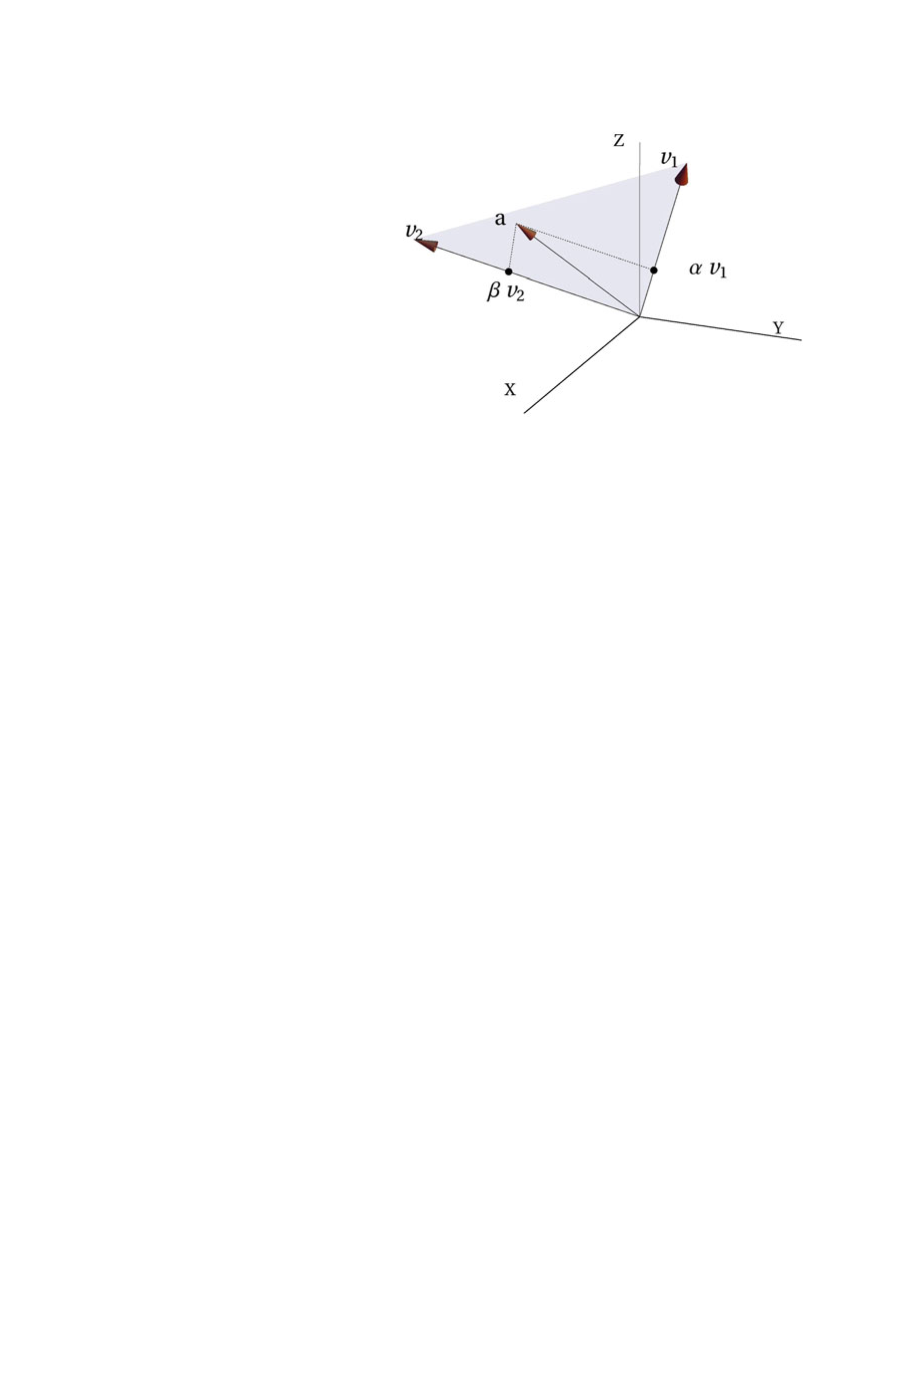
\includegraphics[width=0.5\linewidth]{fig_projection.pdf}
    \caption{الاسقاط التعامدي}
    \label{fig:enter-label}
\end{figure}

بالنظر إلى متجهين مستقلين خطيًا \( a \) و \( b \) في \( \mathbb{R}^n \), نريد إيجاد الإسقاط المتعامد لـ \( a \) على الخط الذي يتولده \( b \). لهذا الغرض, نرمز بـ \( M \) المستوي الذي يتولده \( a \) و \( b \) ونعتبر أساسًا متعامدًا { \( v_1 \), \( v_2 \) } لـ \( M \) يتكون من \( v_1 = \frac{b}{\|b\|} \) ومتجه وحدة \( v_2 \in M \) متعامد على \( v_1 \) (الشكل 1.1). بما أن { \( v_1 \), \( v_2 \) } هو أساس لـ \( M \), هناك أعداد حقيقية \( \alpha \) و \( \beta \) بحيث أن \( a = \alpha v_1 + \beta v_2 \).

الإسقاط لـ \( a \) على الخط الذي يتولده \( b \) هو بالتحديد \( \alpha v_1 \). لتحديد \( \alpha \), نأخذ ببساطة الجداء الداخلي مع \( b \) في الهوية أعلاه. بما أن \( \langle v_1, b \rangle = \|b\| \) و \( \langle v_2, b \rangle = 0 \), نحصل على:
أي أن,
\begin{eqnarray*}
\langle a, b \rangle = \alpha \|b\|.
\\
 \alpha = \frac{\langle a, b \rangle}{\|b\|}
\end{eqnarray*}
تمثل مركبة المتجه \( a \) الموازية للمتجه \( b \). سيكون هذا مفيدًا في الفصل 2 عندما نحسب مركبة القوة في الاتجاه المماسي لمسار معين. لاحظ أنه بهذه الطريقة, يمكننا فعليًا بناء أساس متعامد { \( v_1 \), \( v_2 \) } لـ \( M \) بأخذ:
\begin{eqnarray*}
 v_1 &:=& \frac{b}{\|b\|} \\
 v_2 &:=& \dfrac{a - \dfrac{\langle a, b \rangle}{\|b\|} \dfrac{b}{\|b\|}}{\|a - \dfrac{\langle a, b \rangle}{\|b\|} \frac{b}{\|b\|}\|}. 
\end{eqnarray*}
بالنظر إلى متجهين مستقلين خطيًا \( a \) و \( b \) في \( \mathbb{R}^n \), نريد إيجاد الإسقاط المتعامد لـ \( a \) على الخط الذي يتولده \( b \). لهذا الغرض, نرمز بـ \( M \) المستوي الذي يتولده \( a \) و \( b \) ونعتبر أساسًا متعامدًا { \( v_1 \), \( v_2 \) } لـ \( M \) يتكون من \( v_1 = \frac{b}{\|b\|} \) ومتجه وحدة \( v_2 \in M \) متعامد على \( v_1 \) (الشكل 1.1). بما أن { \( v_1 \), \( v_2 \) } هو أساس لـ \( M \), هناك أعداد حقيقية \( \alpha \) و \( \beta \) بحيث أن \( a = \alpha v_1 + \beta v_2 \).

الإسقاط لـ \( a \) على الخط الذي يتولده \( b \) هو بالتحديد \( \alpha v_1 \). لتحديد \( \alpha \), نأخذ ببساطة الجداء الداخلي مع \( b \) في الهوية أعلاه. بما أن \( \langle v_1, b \rangle = \|b\| \) و \( \langle v_2, b \rangle = 0 \), نحصل على:

أي أن,
\begin{eqnarray*}
\langle a, b \rangle = \alpha \|b\|.
\\
\alpha = \frac{\langle a, b \rangle}{\|b\|}
\end{eqnarray*}
تمثل مركبة المتجه \( a \) الموازية للمتجه \( b \). سيكون هذا مفيدًا في الفصل 2 عندما نحسب مركبة القوة في الاتجاه المماسي لمسار معين. لاحظ أنه بهذه الطريقة, يمكننا فعليًا بناء أساس متعامد { \( v_1 \), \( v_2 \) } لـ \( M \) بأخذ:

\begin{definition}
الضرب الاتجاهي لمتجهين
\[ a = (a_1, a_2, a_3) \text{ و } b = (b_1, b_2, b_3) \]
في \( \mathbb{R}^3 \) هو المتجه المعرف بالتعبير الرسمي

\[ a \times b := \begin{vmatrix} \mathbf{e}_1 & \mathbf{e}_2 & \mathbf{e}_3 \\ a_1 & a_2 & a_3 \\ b_1 & b_2 & b_3 \end{vmatrix}. \]

هنا, \(\{\mathbf{e}_1, \mathbf{e}_2, \mathbf{e}_3\}\) يمثل الأساس المعياري (الشكل 1.2) لـ \( \mathbb{R}^3 \), أي
\[ \mathbf{e}_1 = (1, 0, 0), \mathbf{e}_2 = (0, 1, 0), \mathbf{e}_3 = (0, 0, 1). \]
\end{definition}

ونفسر أن إحداثيات المتجه \( a \times b \) يتم الحصول عليها بعد توسيع المحدد على طول الصف الأول. أي أن,

\[ a \times b := \left( \begin{vmatrix} a_2 & a_3 \\ b_2 & b_3 \end{vmatrix}, -\begin{vmatrix} a_1 & a_3 \\ b_1 & b_3 \end{vmatrix}, \begin{vmatrix} a_1 & a_2 \\ b_1 & b_2 \end{vmatrix} \right). \]

إنها عملية حسابية روتينية ولكنها شاقة للتحقق من أن:

\[ \|a \times b\|^2 = \|a\|^2 \cdot \|b\|^2 - |\langle a, b \rangle|^2 = \|a\|^2 \cdot \|b\|^2 (1 - \cos^2(\theta)) = \|a\|^2 \cdot \|b\|^2 \sin^2(\theta), \]

حيث أن \( \theta \in [0, \pi] \) هي الزاوية بين المتجهين \( a \) و \( b \). بالتالي,

\[ \|a \times b\| = \|a\| \cdot \|b\| \cdot \sin(\theta). \]

\begin{figure}
    \centering
    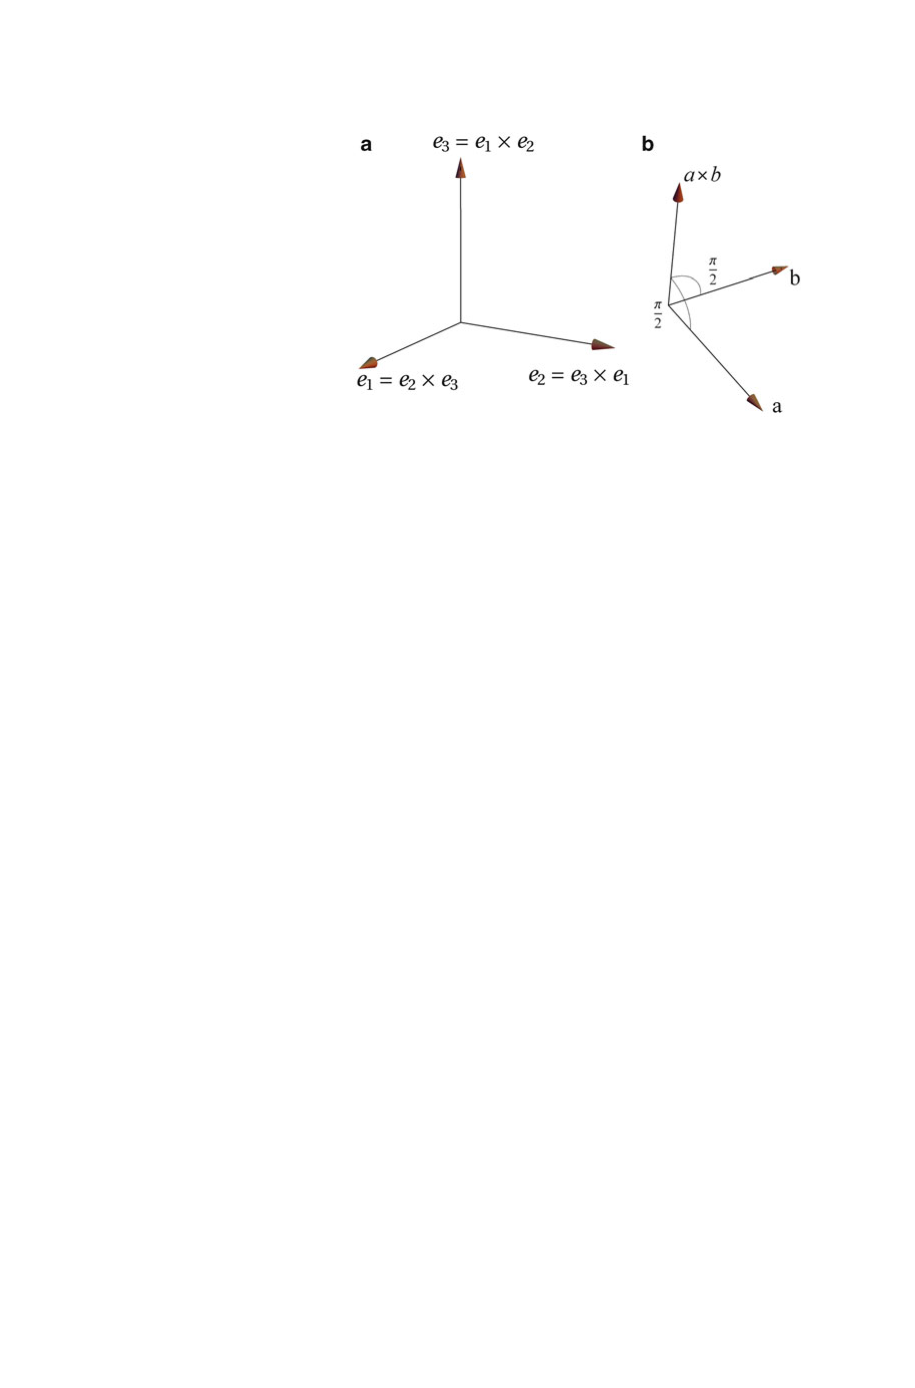
\includegraphics[width=0.5\linewidth]{cross_product.pdf}
    \caption{$(a)$ الاساس المعياري.  $(b)$ الضرب الاتجاهي}
    \label{fig:enter-label}
\end{figure}

إذا كان \( a \) و \( b \) مستقلين خطيًا, فإن هذا التعبير يعطي مساحة متوازي الأضلاع المتولد بواسطة \( a \) و \( b \) (انظر المثال 4.1.1).
\begin{definition}
حاصل الضرب الثلاثي القياسي لثلاثة متجهات \( a \), \( b \), و \( c \) في \( \mathbb{R}^3 \) هو العدد القياسي المعرف بـ
\[ \langle a, b \times c \rangle. \]
إذا كتبنا:
\[ a = (a_1, a_2, a_3), b = (b_1, b_2, b_3), c = (c_1, c_2, c_3), \]
فإنه يتبع من التعاريف أن:
\[ \langle a, b \times c \rangle = a_1 \begin{vmatrix} b_2 & b_3 \\ c_2 & c_3 \end{vmatrix} - a_2 \begin{vmatrix} b_1 & b_3 \\ c_1 & c_3 \end{vmatrix} + a_3 \begin{vmatrix} b_1 & b_2 \\ c_1 & c_2 \end{vmatrix} = \begin{vmatrix} a_1 & a_2 & a_3 \\ b_1 & b_2 & b_3 \\ c_1 & c_2 & c_3 \end{vmatrix}. \]
\end{definition}
من خواص المحددات, نحصل فورًا على الخواص التالية للضرب الاتجاهي لمتجهين.

\begin{theoreme}
يتمتع الضرب الاتجاهي بالخصائص التالية:
\begin{itemize}
    \item [(1)] \( b \times a = - (a \times b) \).
    \item [(2)] \( a \times b \) متعامد على المتجهين \( a \) و\( b \).
    \item [(3)] \( a \) و\( b \) مستقلان خطيًا إذا وفقط إذا كان \( a \times b \neq 0 \).
\end{itemize}
\end{theoreme}

الضرب الاتجاهي للمتجهات في \( \mathbb{R}^2 \) غير معرف. ومع ذلك, كما سنرى في القسم 7.2, من الممكن تعريف الضرب الاتجاهي لـ \( n - 1 \) متجهات في \( \mathbb{R}^n \) عندما يكون \( n \geq 3 \).
يتمتع حاصل الضرب الثلاثي القياسي أيضًا بتفسير هندسي مثير للاهتمام. لنفترض أن \( a \), \( b \), و\( c \in \mathbb{R}^3 \) هي ثلاثة متجهات مستقلة خطيًا. هذه المتجهات تولد متوازي مستطيلات, قاعدته يمكن أن تكون متوازي الأضلاع الذي يتولده \( a \) و\( b \) (انظر الشكل 1.3). المتجه \( a \times b \) متعامد على المستوى الذي يتولده \( a \) و\( b \), ونتيجة لذلك, ارتفاع هذا المتوازي المستطيلات (بالنسبة للمستوى المذكور) يتزامن مع مركبة \( c \) الموازية لاتجاه \( \pm (a \times b) \). أي أن الارتفاع يعطى بـ
\[ h = \left| \frac{\langle c, a \times b \rangle}{\|a \times b\|} \right|. \]
يمكن الآن حساب حجم متوازي المستطيلات عن طريق:
\[ الحجم = القاعدة \times الارتفاع = \|a \times b\| \cdot h = |\langle c, a \times b \rangle| = |\langle a, b \times c \rangle|. \]


\begin{figure}
    \centering
    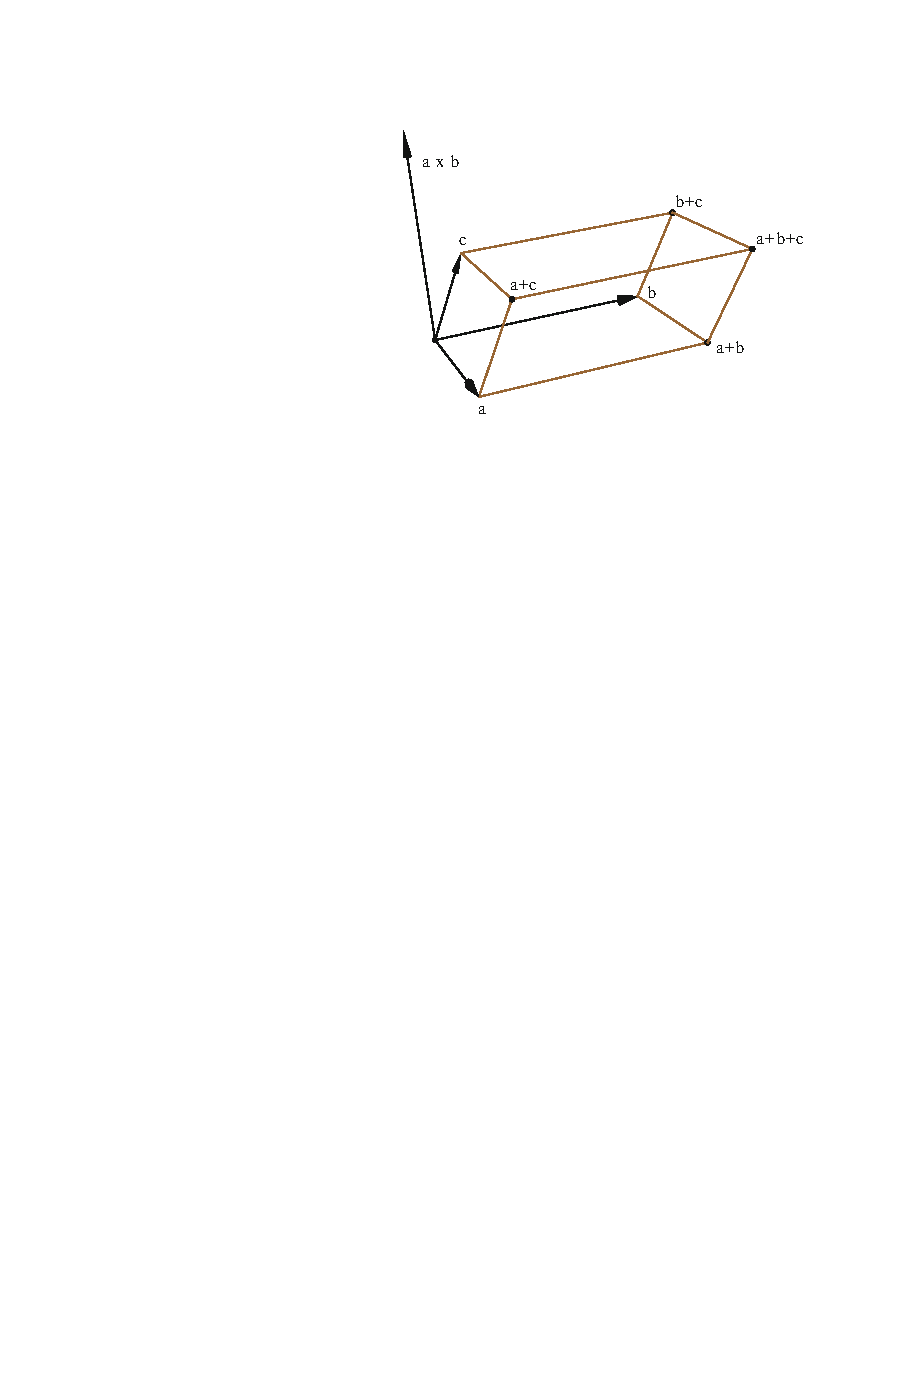
\includegraphics[width=0.5\linewidth]{Parallelepiped.pdf}
    \caption{متوازي مستطيلات يتولد بواسطة ثلاثة متجهات}
    \label{fig:enter-label}
\end{figure}

لذلك, حجم متوازي المستطيلات هو القيمة المطلقة لحاصل الضرب الثلاثي القياسي للمتجهات الثلاثة. سنعمم هذه النتيجة لاحقاً.
\newpage
\section{ الحقول المتجهة}

على مدار هذه الملخصات, نفترض أن الطالب لديه معرفة أساسية بالتفاضل والتكامل في عدة متغيرات, ولكن من أجل التناسق, سنستذكر التعريفات والنتائج ذات الصلة.

\begin{definition}
لنفترض أن \(a \in \mathbb{R}^n\), فإن الكرة المفتوحة ذات المركز \(a\) ونصف القطر \(r > 0\) هي المجموعة
\[ B(a, r) = \{x \in \mathbb{R}^n : \|x - a\| < r\}. \]
الكرة المغلقة ذات المركز \(a\) ونصف القطر \(r \geq 0\) هي المجموعة
\[ 
D(a, r) = \{x \in \mathbb{R}^n : \|x - a\| \leq r\}. 
\]
\end{definition}

\begin{definition}
\begin{itemize}
    \item [(i)] تُسمى مجموعة فرعية \(U\) من \(\mathbb{R}^n\) مفتوحة إذا لكل \(x \in U\) يوجد \(r > 0\) (يعتمد على \(x\)) بحيث \(B(x, r) \subset U\).
    \item [(ii)] تُسمى مجموعة \(C\) في \(\mathbb{R}^n\) مغلقة إذا كان متممها \(\mathbb{R}^n \setminus C\) مجموعة مفتوحة.
    \item [(iii)] لنفترض \(a \in \mathbb{R}^n\), تُسمى مجموعة \(G \subset \mathbb{R}^n\) حيًا لـ\(a\) إذا كان هناك \(r > 0\) بحيث تكون الكرة \(B(a, r)\) محتواة في \(G\). على وجه الخصوص, إذا كانت المجموعة \(G\) مفتوحة, فهي حي مفتوح لجميع نقاطها.
    \item[(iv)] إذا كانت \(A\) مجموعة فرعية من \(\mathbb{R}^n\), فإن داخل \(A\) هو المجموعة
    \[ 
    \operatorname{int}(A) := \{x \in A : A \text{ هو حي لـ } x\}.
    \]
    \item [(v)] إغلاق \(A\) هو المجموعة
    \[ 
    \bar{A} := \{x \in \mathbb{R}^n : B(x, r) \cap A \neq \emptyset \text{ لكل } r > 0\}. \]
\end{itemize}
\end{definition}

أي كرة مفتوحة \(B(a, r)\) هي مجموعة مفتوحة. في الواقع, إذا \(x \in B(a, r)\), فإن متباينات المثلث تعني أن \(B(x, r - \|x - a\|)\) هي كرة مفتوحة ذات المركز \(x\) محتواة في \(B(a, r)\). وبالمثل, فإن أي كرة مغلقة هي مجموعة مغلقة. بصفة عامة, مجموعة \(A\) مفتوحة إذا وفقط إذا كانت تتطابق مع داخلها, \(\operatorname{int}(A)\), وتكون مغلقة إذا وفقط إذا كانت تتطابق مع إغلاقها \(\bar{A}\).

نستذكر الآن مفاهيم الخرائط المستمرة والقابلة للتفاضل.

\begin{definition}
    
لنفترض أن \(M\) مجموعة فرعية من \(\mathbb{R}^n\). تخطيط \(f : M \subset \mathbb{R}^n \to \mathbb{R}^m\) تكون مستمرة عند نقطة \(a \in M\) إذا لكل \(\epsilon > 0\) يوجد \(\delta > 0\) بحيث لكل \(x \in M\) مع \(\|x - a\| < \delta\), لدينا
\[ \|f(x) - f(a)\| < \epsilon. \]
\end{definition}

نقول أن \(f\) مستمرة على \(M\) إذا كانت مستمرة عند كل نقطة من \(M\). عادةً عندما يكون مجال الصورة هو \(\mathbb{R}\) سنقول أن \(f\) دالة مستمرة.

\begin{definition}
لنفترض أن \(M\) مجموعة فرعية من \(\mathbb{R}^n\) ونعتبر \(a \in M\) التي تحتوي على خاصية أن \(M \cap (B(a, r) \setminus \{a\}) \neq \emptyset\) لكل \(r > 0\). نقول أن التخطيط \(f : M \subset \mathbb{R}^n \to \mathbb{R}^m\) لها حد \(b \in \mathbb{R}^m\) عند النقطة \(a\), ونكتب \(\lim_{x \to a} f(x) = b\), إذا لكل \(\epsilon > 0\) يوجد \(\delta > 0\) بحيث لكل \(x \in M\) مع \(\|x - a\| < \delta\), لدينا
\[ \|f(x) - b\| < \epsilon. \]
\end{definition}

\begin{definition}
    
لنفترض أن \(f : U \subset \mathbb{R}^n \to \mathbb{R}\) دالة معرفة على المجموعة المفتوحة \(U\). نقول أن \(f\) لديها مشتق جزئي في الإحداثي \(i\) عند \(a \in U\) إذا كان الحد
\[ \lim_{h \to 0} \frac{f(a_1, \ldots, a_{i-1}, a_i + h, a_{i+1}, \ldots, a_n) - f(a_1, \ldots, a_n)}{h} \]
موجودًا, وعندما يكون الحد موجودًا, سنرمز قيمته (وهو عدد حقيقي) بـ \(\frac{\partial f}{\partial x_i}(a)\).
\end{definition}

بصفة عامة, لـ \(f : U \subset \mathbb{R}^n \to \mathbb{R}^m\) و \(v \in \mathbb{R}^n\), نحدد المشتق الاتجاهي لـ \(f\) عند \(a \in U\) في الاتجاه \(v\) ليكون
\[ D_v f(a) = \lim_{t \to 0} \frac{f(a + tv) - f(a)}{t}, \]
عندما يكون هذا الحد موجودًا.

\begin{definition}
لنفترض أن \(f : U \subset \mathbb{R}^n \to \mathbb{R}^m\)تخطيط معرف  على المجموعة المفتوحة \(U\). نقول أن \(f\) قابلة للتفاضل عند \(a \in U\) إذا كانت هناك تخطيط خطي  \(T : \mathbb{R}^n \to \mathbb{R}^m\) بحيث
\[ \lim_{h \to 0} \frac{f(a + h) - f(a) - T(h)}{\|h\|} = 0. \]
في هذه الحالة, نرمز التخطيط الخطي الوحيد \(T\) بـ \(df(a)\). نقول أن \(f\) قابلة للتفاضل على \(U\) إذا كانت قابلة للتفاضل عند كل نقطة من \(U\).

تخطيط \(f : U \subset \mathbb{R}^n \to \mathbb{R}^m\), \(f = (f_1, \ldots, f_m)\), قابلة للتفاضل عند \(a \in U\) إذا وفقط إذا كانت كل دالة إحداثية \(f_j\) قابل للتفاضل عند \(a\). إذا رمزنا لمصفوفة \(df(a)\) (بالنسبة للأساس القانوني) بـ \(f'(a)\), يكون لدينا
\[ f'(a) = \begin{pmatrix}
\frac{\partial f_1}{\partial x_1}(a) & \frac{\partial f_1}{\partial x_2}(a) & \cdots & \frac{\partial f_1}{\partial x_n}(a) \\
\frac{\partial f_2}{\partial x_1}(a) & \frac{\partial f_2}{\partial x_2}(a) & \cdots & \frac{\partial f_2}{\partial x_n}(a) \\
\vdots & \vdots & \ddots & \vdots \\
\frac{\partial f_m}{\partial x_1}(a) & \frac{\partial f_m}{\partial x_2}(a) & \cdots & \frac{\partial f_m}{\partial x_n}(a)
\end{pmatrix}. \]
\end{definition}

 \(f'(a)\) تسمى
 مصفوفة الجاكوبيان او اليعقوبي لـ
\(f\) عند \(a\) وفي حالة \(m = n\), يُسمى محددها بـ يعقوبي لـ \(f\) عند \(a\) ويرمز له بـ \(J_f(a)\).

في حالة الدالة ذات القيمة العددية حيث \( f : U \subset \mathbb{R}^n \to \mathbb{R} \) قابلة للتفاضل عند \( a \), يُسمى \( f'(a) \) تدرج \( f \) عند \( a \). عادة ما يُرمز إليه بـ \( \nabla f(a) \) ويُعامل كمتجه صف في \( \mathbb{R}^n \), أي:
\[ \nabla f(a) = \left( \frac{\partial f}{\partial x_1} (a), \frac{\partial f}{\partial x_2} (a), \ldots, \frac{\partial f}{\partial x_n} (a) \right). \]

هي أنه إذا كانت الدالة \( f : U \subset \mathbb{R}^n \to \mathbb{R}^m \) قابلة للتفاضل عند \( a \in U \), فإن المشتقة الاتجاهية لـ \( f \) عند \( a \) في اتجاه \( v \) موجودة لكل \( v \in \mathbb{R}^n \) وتكون:
\[ D_v f(a) = df(a)(v). \]

الشرط للتفاضل المعطى في التعريف اعلاه ليس من السهل التحقق منه, ولكن النظرية التالية, التي يمكن العثور عليها في أي كتاب دراسي عن حساب التفاضل في عدة متغيرات, تقدم شرطًا كافيًا أكثر ملاءمة. نحتاج أولاً إلى تعريف آخر.

\begin{definition}
لنفترض أن \( f : U \subset \mathbb{R}^n \to \mathbb{R}^m \) دالة معرفة على المجموعة المفتوحة \( U \). نقول أن \( f \) قابلة للتفاضل باستمرار عند \( a \in U \) إذا كان هناك \( r > 0 \) بحيث تكون الكرة \( B(a, r) \) محتواة في \( U \) وجميع المشتقات الجزئية \( \frac{\partial f_i}{\partial x_j}(x) \) ( \( i = 1, \ldots, m \), \( j = 1, \ldots, n \) ) موجودة في الكرة ومستمرّة عند \( a \). ثم يُقال أن \( f \) من الفئة \( C^1 \) على \( U \) إذا كانت قابلة للتفاضل باستمرار عند جميع نقاط \( U \).
\end{definition}

\begin{theoreme}
إذا كانت \( f : U \subset \mathbb{R}^n \to \mathbb{R}^m \) دالة قابلة للتفاضل باستمرار عند نقطة \( a \) في مجموعة مفتوحة \( U \), فإن \( f \) قابلة للتفاضل عند \( a \). على وجه الخصوص, إذا كانت \( f \) من الفئة \( C^1 \) على المجموعة المفتوحة \( U \), فإن \( f \) قابلة للتفاضل على \( U \).
\end{theoreme}

إذا كانت \( f : U \subset \mathbb{R}^n \to \mathbb{R}^m \) دالة من الفئة \( C^1 \) على مجموعة مفتوحة \( U \), يمكننا النظر في الدوال المستمرة \( \frac{\partial f_i}{\partial x_j} : U \to \mathcal{R} \). سنقول أن \( f \) من الفئة \( C^2 \) على \( U \) إذا كانت كل \( \frac{\partial f_i}{\partial x_j} : U \to \mathcal{R} \) من الفئة \( C^1 \) على \( U \)
اذا كان كل
\[\frac{\partial f_i}{\partial x_j} : U \to \mathcal{R}\] 
هي فئة $C^1$ عل $U$, بمعني ان 
\[
\frac{\partial^2f_i}{\partial x_k \partial x_j}(x).
\]

يمكن بوضوح تكرار هذه العملية لتعريف دالة من الفئة \( C^p \) على \( U \). إذا كانت \( f \) من الفئة \( C^p \) لكل \( p \in \mathbb{N} \), فإننا نقول إنها من الفئة \( C^\infty \) على \( U \).

\begin{definition}
حقل المتجهات هو دالة مستمرة
\[ F : U \subset \mathbb{R}^n \to \mathbb{R}^n. \]
\end{definition}

\begin{figure}
    \centering
    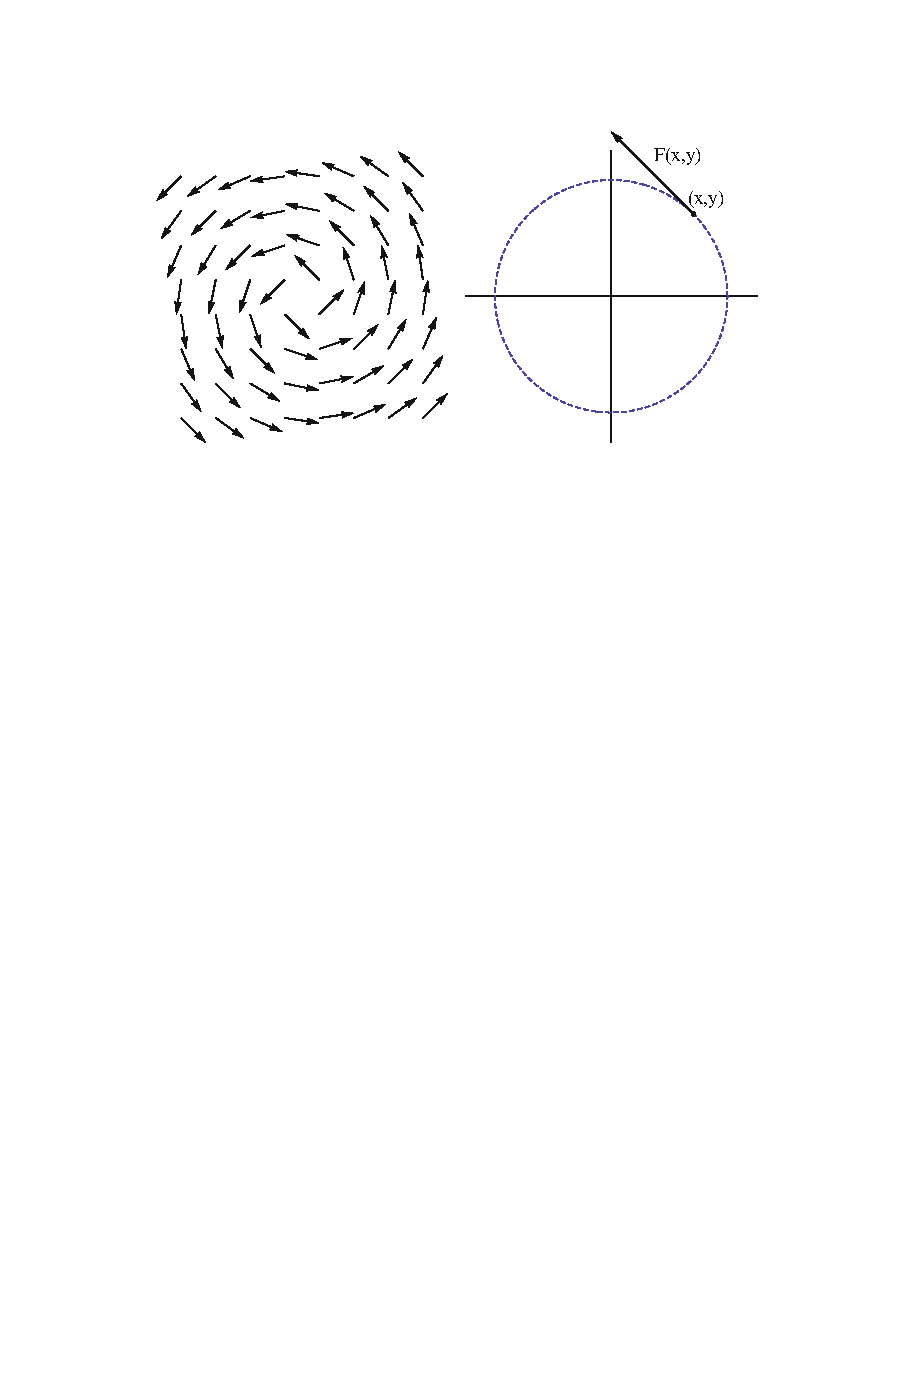
\includegraphics[width=0.8\linewidth]{vector field.pdf}
    \caption{مثال لحقل متحهات}
    \label{fig:enter-label}
\end{figure}

التفسير الطبيعي لهذا التعريف هو أن حقل المتجهات يخصص متجهًا لنقطة. حقول المتجهات مفيدة في تمثيل حقول القوة أو حقول السرعة. سيجد طالب الرياضيات في دراسته العديد من الحالات لهذا الموقف حيث يمكن تفسير نفس المفهوم المجرد بطرق مختلفة من خلال الجهاز البسيط لتغيير اسم ذلك المفهوم. هنا تصبح دالة من \( \mathbb{R}^n \) إلى نفسها مفهومًا فيزيائيًا, فقط من خلال تسميتها حقل متجهات, وبالتالي يتم تصورها بطريقة جديدة, كما توضح الأمثلة التالية.

\begin{exemple}
لننظر في حقل المتجهات (الشكل 1.4)
\[ F : \mathbb{R}^2 \setminus \{0\} \to \mathbb{R}^2 \]
المعرف بواسطة
\[ F(x, y) = \left( -\frac{y}{x^2 + y^2}, \frac{x}{x^2 + y^2} \right). \]

بوضوح, \( F(x, y) \) هو متجه وحدة, وإذا وضعنا هذا المتجه عند النقطة (x, y), نرى أنه متجه مماسي عند (x, y) للدائرة المتمركزة عند الأصل التي تمر بهذه النقطة.
\end{exemple}

\begin{exemple}[(حقول الجاذبية)]
لننظر في جسيم كتلته \( M \) موجود عند الأصل. قوة الجذب المؤثرة على جسيم كتلته \( m \) موجود عند \( (x, y, z) \in \mathbb{R}^3 \setminus \{0\} \) هي
\[ F(x, y, z) = - \frac{GMm}{(x^2 + y^2 + z^2)^{3/2}} (x, y, z), \]
حيث \( G \) هو ثابت الجاذبية و \( \mathbf{u} = \frac{(x, y, z)}{\sqrt{x^2 + y^2 + z^2}} \) هو متجه وحدة في الاتجاه من الأصل إلى (x, y, z). أي أن المتجه \( F(x, y, z) \) يشير دائمًا من (x, y, z) نحو الأصل, ومقداره يتناسب عكسيًا مع مربع المسافة إلى الأصل (الشكل 1.5).
\end{exemple}

\begin{figure}
    \centering
    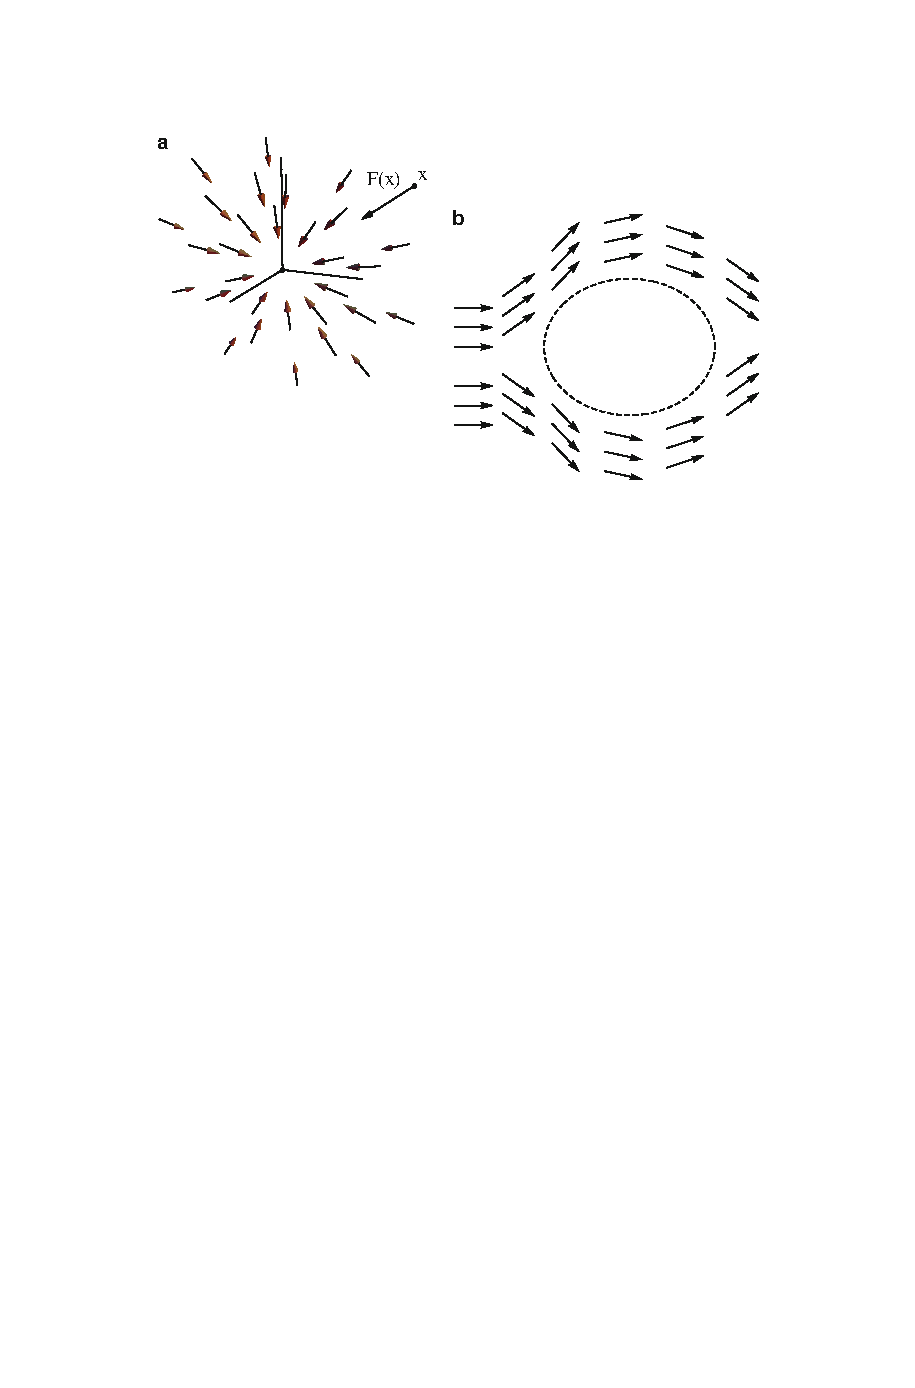
\includegraphics[width=0.8\linewidth]{Gravitational field.pdf}
    \caption{$a$  حقل متجهات        $b$ حركة جزي في مائع}
    \label{fig:enter-label}
\end{figure}

\begin{exemple}[(حقل السرعة لسائل)]

لكل نقطة \((x, y, z)\) من مجموعة مفتوحة \( U \subset \mathbb{R}^3 \) لنفترض أن \( F(x, y, z) \) تمثل سرعة سائل في الموضع \((x, y, z)\) عند زمن معين. إذن
\[ 
F : U \subset \mathbb{R}^3 \to \mathbb{R}^3 
\]
هو حقل متجهات.
\end{exemple}

\begin{exemple}

لنفترض أن
\[ g : U \subset \mathbb{R}^n \to \mathbb{R} \]
دالة من الفئة \( C^1 \) على المجموعة المفتوحة \( U \). إذن
\[ F := \nabla g : U \to \mathbb{R}^n, F(x) = \nabla g(x) := \left( \frac{\partial g}{\partial x_1}, \ldots, \frac{\partial g}{\partial x_n} \right) \]
هو حقل متجهات ويُسمى حقل التدرج لـ \( g \).
\end{exemple}

\begin{definition}
 
لنفترض أن \( \mathcal{F} : U \subset \mathbb{R}^n \to \mathbb{R}^n \) حقل متجهات بمكونات \( F = (f_1, f_2, \ldots, f_n) \). نتذكر أن \( F \) من الفئة \( C^p \) (أو قابل للتفاضل) على المجموعة المفتوحة \( U \) إذا كانت كل من مكوناته \( f_j \) من الفئة \( C^p \) (أو قابلة للتفاضل).
\end{definition}

بعد ذلك, نقدم عمليتين أساسيتين على حقول المتجهات؛ التباعد (وهو دالة عددية) والتدوير, أو الروتور (وهو حقل متجهات). يلعبان دورًا مركزيًا في صياغة نظريتين أساسيتين في التحليل المتجهي, وهما نظرية التباعد, أو نظرية غاوس, ونظرية ستوكس الكلاسيكية.  

\begin{definition}
لنفترض أن \( F : U \subset \mathbb{R}^n \to \mathbb{R}^n \) هو حقل متجهات من الفئة \( C^1 \) على المجموعة المفتوحة \( U \). التباعد \( \text{Div} \) لـ \( F \) هو الدالة العددية
\[ \text{Div} \, F = \sum_{j=1}^{n} \frac{\partial f_j}{\partial x_j}. \]
\end{definition}

\begin{definition}
لنفترض أن \( F : U \subset \mathbb{R}^3 \to \mathcal{R}^3, F = (f_1, f_2, f_3) \), هو حقل متجهات من الفئة \( C^1 \) على المجموعة المفتوحة \( U \). التدوير (أو الروتور) لـ \( F \) هو حقل المتجهات المعرف, رسميًا, بالمحدد
\begin{eqnarray*}
    \text{Curl} \, F = \begin{vmatrix} \mathbf{e}_1 & \mathbf{e}_2 & \mathbf{e}_3 \\ \frac{\partial}{\partial x} & \frac{\partial}{\partial y} & \frac{\partial}{\partial z} \\ 
    f_1 & f_2 & f_3 \end{vmatrix}. 
\end{eqnarray*}
\end{definition}

نفسر أن مكونات \( \text{Curl} \, F \) يتم الحصول عليها بعد توسيع المحدد على طول الصف الأول. وبالتالي, يكون \( \text{Curl} \, F \) هو حقل المتجهات

\begin{eqnarray*}
    \text{Curl} \, F &=& \left( \frac{\partial f_3}{\partial y} - \frac{\partial f_2}{\partial z}, \frac{\partial f_1}{\partial z} - \frac{\partial f_3}{\partial x}, \frac{\partial f_2}{\partial x} - \frac{\partial f_1}{\partial y} \right).
\end{eqnarray*}

عادةً ما نضع \( \nabla \) لتمثيل المؤثر التفاضلي

\[ \nabla = \left( \frac{\partial}{\partial x}, \frac{\partial}{\partial y}, \frac{\partial}{\partial z} \right). \]

هذا, مع ترميز الضرب الاتجاهي في التعريف 1.1.4, يقترح التمثيل الرمزي التالي لتدوير \( F \):

\[ \text{Curl} \, F = \nabla \times F. \]

نلاحظ أن التباعد معرّف لحقول المتجهات في \( \mathcal{R}^n \), بينما التدوير معرّف فقط لحقول المتجهات في \( \mathcal{R}^3 \).

\begin{figure}
    \centering
    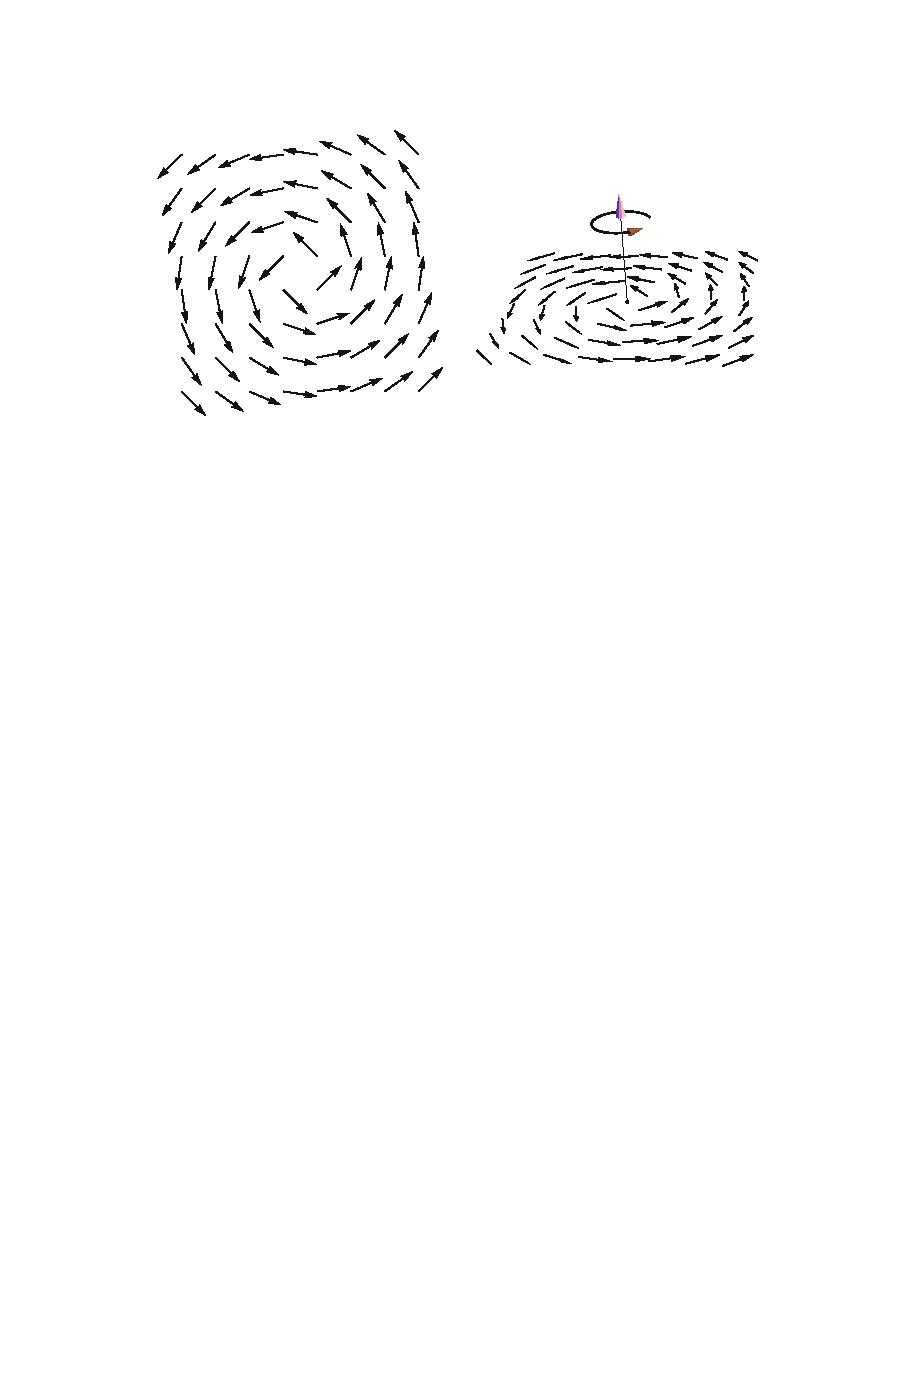
\includegraphics[width=0.8\linewidth]{Vector field Example.pdf}
    \caption{حقل متجهات}
    \label{fig:enter-label}
\end{figure}

\begin{exemple}
حقل المتجهات \( F(x, y, z) = (-y, x, 0) \) يمثل دورانًا حول \( N = (0, 0, 1) \). نلاحظ أن 
\( \text{Curl} \, F = (0, 0, 1) \) يعطي اتجاه محور الدوران (انظر الشكل 1.6). سنستنتج من نظرية ستوكس أن هذا ليس صدفة (انظر النتيجة 9.4.1).
\end{exemple}

بعد ذلك نسلط الضوء على علاقة مهمة بين التباعد والتدوير, ولكن لذلك, نحتاج إلى النظرية التالية المنسوبة إلى شوارتز حول تماثل المشتقات الثانية لدالة من الفئة \( C^2 \). يُطلق عليها أحيانًا أيضًا نظرية كليرو أو نظرية يونغ.

\begin{theoreme}
لنفترض أن \( f : U \subset \mathbb{R}^n \to \mathbb{R} \) دالة من الفئة \( C^2 \) على المجموعة المفتوحة \( U \). إذن, لكل \( x \in U \) ولكل \( i, j = 1, 2, \cdots, n \),
\[ 
\frac{\partial^2 f}{\partial x_i \partial x_j} (x) = \frac{\partial^2 f}{\partial x_j \partial x_i} (x). 
\]
\end{theoreme}

\begin{theoreme}

لنفترض أن \( F : U \subset \mathcal{R}^3 \to \mathcal{R}^3 \) هو حقل متجهات من الفئة \( C^2 \) على المجموعة المفتوحة \( U \). إذن,
\[
\text{Div} (\text{Curl} \, F) = 0.
\]
\end{theoreme}
\begin{demonstration}

نظرًا لأن \( F = (f_1, f_2, f_3) \), فإن نظرية شوارتز حول تماثل المشتقات الثانية تعطي:
\[ \text{Div} (\text{Curl} \, F) = \frac{\partial}{\partial x} \left( \frac{\partial f_3}{\partial y} - \frac{\partial f_2}{\partial z} \right) + \frac{\partial}{\partial y} \left( \frac{\partial f_1}{\partial z} - \frac{\partial f_3}{\partial x} \right) + \frac{\partial}{\partial z} \left( \frac{\partial f_2}{\partial x} - \frac{\partial f_1}{\partial y} \right). \]
باستخدام نظرية شوارتز نحصل على:
\[ = \frac{\partial^2 f_3}{\partial x \partial y} - \frac{\partial^2 f_2}{\partial x \partial z} + \frac{\partial^2 f_1}{\partial y \partial z} - \frac{\partial^2 f_3}{\partial y \partial x} + \frac{\partial^2 f_2}{\partial z \partial x} - \frac{\partial^2 f_1}{\partial z \partial y} = 0. \]
\end{demonstration}

    
\section{تمارين}

\begin{exercice}
 تحقق من أن
\[ \text{Div} (\text{Curl} F) = 0 \]
للحقل المتجه التالي:
\[ F(x, y, z) = (x^2z, x, 2yz) \]
\end{exercice}

\begin{exercice}
    احسب التباعد والدوران عند النقطة \((1, 1, 0)\) للحقل المتجه التالي:
\[ F(x, y, z) = (xyz, y, z). \]
\end{exercice}

\begin{exercice}
احسب التباعد للحقلين المتجهين التاليين:
\begin{enumerate}[start=3]
\item [1.] \( F(x, y) = (\sin(x), e^{x-y}) \).
\item [2.] \( F(x, y, z) = (\sin(y), \cos(z), z^3) \).
 \end{enumerate}
\end{exercice}

\begin{exercice}
    ليكن \( F : \mathbb{R}^3 \to \mathbb{R}^3 \) حقل متجه وليكن \( g : \mathbb{R}^3 \to \mathbb{R} \) دالة عددية, كلاهما من الفئة \( C^1 \) على \(\mathbb{R}^3\). تحقق من أن
\[ \text{Curl} (gF) = g(\text{Curl} F) + (\nabla g) \times F \].
\end{exercice}

\begin{exercice} 
إذا كانت \( F, G : \mathbb{R}^3 \to \mathbb{R}^3 \) حقول متجهة من الفئة \( C^1 \), أثبت أن
\[ \text{Div} (F \times G) = \langle \text{Curl} F, G \rangle - \langle F, \text{Curl} G \rangle \].
\end{exercice}

 \chapter{التكاملات الخطية}

في دراسة حركة جسيم على طول قوس, يكون من الملائم اعتبار القوس كصورة لدالة متجهية القيمة \( \gamma : [a, b] \to \mathbb{R}^3 \) معرفة على فترة من الخط الحقيقي وتحقيق \( \gamma(t) \) كموضع الجسيم عند الزمن \( t \). هذا المنظور يكون أيضًا ملائمًا في تحليل سلوك حقل المتجهات على طول القوس وهو الدافع الرئيسي للتعاريف التالية.

\section{ المسارات}

\begin{definition}
المسار هو دالة مستمرة \( \gamma : [a, b] \to \mathbb{R}^n \). نسمي \( \gamma(a) \) النقطة الابتدائية و \( \gamma(b) \) النقطة النهائية. تُسمى صورة المسار \( \gamma([a, b]) \) قوسًا لـ \( \gamma \). إذا كانت \( \gamma([a, b]) \subset \Omega \), نقول إن \( \gamma \) مسار في \( \Omega \).
\end{definition}

\begin{exemple}
قطعة الخط التي تصل بين نقطتين \( x \) و \( y \) في \( \mathbb{R}^n \) هي القوس \([x, y] := \gamma([0, 1])\), حيث \( \gamma : [0, 1] \to \mathbb{R}^n \) تدل على المسار
\[ \gamma(t) = x + t(y - x) = ty + (1 - t)x. \]
\end{exemple}

\begin{exemple}
لنفترض أن \( \gamma_j : [0, 2\pi] \to \mathbb{R}^2 \) معطاة بواسطة \( \gamma_j(t) := (\cos(jt), \sin(jt)) \). إذن لكل \( j \in \mathcal{Z} \setminus \{0\} \), فإن القوس \( \gamma_j([0, 2\pi]) \) هو الدائرة الوحدة \( x^2 + y^2 = 1 \) في \( \mathbb{R}^2 \). مع زيادة المعلمة \( t \) من 0 إلى 2\(\pi\), تتحرك النقطة \( \gamma_j(t) \) حول دائرة الوحدة بعدد المرات \( |j| \) (في اتجاه عقارب الساعة عندما يكون \( j \) سالبًا وعكس اتجاه عقارب الساعة عندما يكون \( j \) موجبًا).
\end{exemple}
نضع 
\[
\gamma'(t) := \lim_{h \to t, h \in [a, b]} \frac{\gamma(h) - \gamma(t)}{h - t} 
\]

إذا كانت النهاية موجودة. نلاحظ أنه إذا كان \( t \in (a, b) \), فإن \( \gamma'(t) \) موجود إذا وفقط إذا كانت \( \gamma \) دالة قابلة للتفاضل عند النقطة \( t \). في هذه الحالة, يكون \( \gamma'(t) \) هو مصفوفة عمود \( n \times 1 \) للتفاضل عند \( t \), والتي تُرى بطبيعة الحال كمتجه في \( \mathbb{R}^n \). على وجه الخصوص, يمكننا اعتبار \( \gamma' : [a, b] \to \mathbb{R}^n \), وحيثما كانت الحدود المناسبة موجودة, نكرر لاشتقاق مشتقات أعلى رتبة لـ \( \gamma \). هذا يؤدي إلى التعريفات التالية.

\begin{definition}
    
يُقال إن مسارًا \( \gamma : [a, b] \to \mathbb{R}^n \) هو دالة من الفئة \( C^q \) على $[a,b]$ إذا كانت المشتقة من الرتبة \( q \) \( \gamma^{(q)}(t) \) موجودة لكل \( t \in [a, b] \) وكانت \( \gamma^{(q)} \) مستمرة على $[a,b]$. يُقال إن الدالة \( \gamma \) دالة من قطعة إلى قطعة من الفئة \( C^q \) إذا كانت هناك تقسيمات \( a = t_1 < \cdots < t_k = b \) بحيث تكون \( \gamma|_{[t_i, t_{i+1}]} \) من الفئة \( C^q \) على \(\left[t_i,t_{i+1}\right]\) لكل $1\leq i < k-1$.
\end{definition}

\begin{definition}
    
يُقال إن مسارًا \( \gamma : [a, b] \to \mathbb{R}^n \) أملس إذا كانت \( \gamma \) دالة من الفئة \( C^1 \) وكانت \( \gamma'(t) \neq 0 \) لكل \( t \in [a, b] \).
\end{definition}

\begin{lemma}
لنفترض أن \( c \) عدد حقيقي. الدالة \( f : \mathbb{R} \to \mathbb{R} \),
\[ f(t) := \begin{cases} -c e^{-1/t^2}, t < 0, \\ 0, t = 0, \\ c e^{-1/t^2}, t > 0, \end{cases} \]
هي من الفئة \( C^\infty \) على الخط الحقيقي.
\end{lemma}

\begin{demonstration}[5]

نثبت أنه لكل \( n \in \mathcal{N} \cup \{0\} \) هناك متعددة حدود \( P_n \) بحيث
\[ f^{(n)}(t) := \begin{cases} P_n(t) e^{-1/t^2}, t < 0, \\ 0, t = 0, \\ P_n(t) e^{-1/t^2}, t > 0. \end{cases} \]

في الواقع, هذا واضح بالنسبة لـ \( n = 0 \). لتطبيق الاستقراء, نفترض أن النتيجة صحيحة لـ \( n = k \in \mathcal{N} \cup \{0\} \). لاستنتاج أن النتيجة صحيحة أيضًا لـ \( n = k + 1 \), يكفي التحقق من أن \( f^{(k+1)}(0) = 0 \). سنستخدم أن \( e^{y^2} \) يتباعد إلى ما لا نهاية أسرع من أي متعددة حدود في \( y \) عندما يتجه \( y \) إلى \( +\infty \). في الواقع, إذا كانت \( P_n(y) = a_n y^n + \cdots + a_1 y + a_0 \) مع \( a_n \neq 0 \), فإن
\[ \frac{P_n(y)}{e^{y^2}} = \frac{P_n(y)}{e^{y^2 - y}} \cdot \frac{1}{e^y}. \]

الدالة \( e^{-y^2 + y} \) بوضوح تتقارب إلى الصفر. من ناحية أخرى, بتطبيق قاعدة لوبتال \( n \) مرة, نحصل على
\[ \lim_{y \to +\infty} \frac{P_n(y)}{e^{y^2}} = \frac{a_n}{n!} \lim_{y \to +\infty} \frac{1}{e^y} = 0. \]

الآن بأخذ \( y = 1 \) عندما \( t > 0 \) أو \( y = -1 \) إذا \( t < 0 \) نحصل على
\[ f^{(k+1)}(0) = \lim_{t \to 0} \frac{f^{(k)}(t) - f^{(k)}(0)}{t} = \lim_{t \to 0} \frac{f^{(k)}(t)}{t} = 0. \]
\end{demonstration}

\begin{exemple}
لنفترض أن \( \gamma : [−1, 1] \to \mathbb{R}^2 \) معرّف بواسطة
\[ \gamma(t) := \begin{cases} \left( -e^{1/t^2}, e^{1/t^2} \right), −1 \leq t < 0, \\ (0, 0), t = 0, \\ \left( e^{1/t^2}, e^{1/t^2} \right), 0 < t \leq 1. \end{cases} \]
\end{exemple}

يتبع من التوطئة أعلاه أن \( \gamma \) هو مسار من الفئة \( C^\infty \). ومع ذلك, فإن \( \gamma \) ليس أملسًا, حيث أن \( \gamma'(0) = (0, 0) \). نلاحظ أن \( \gamma([−1, 1]) = \{(x, |x|) : x \in [−1, 1]\} \) له زاوية عند النقطة $(0,0)$. يمكن العثور على عدة أمثلة أخرى في.

مهمتنا التالية هي تعريف, وإذا أمكن, تقييم طول مسار \( \gamma : [a, b] \to \mathbb{R}^n \). الفكرة الأساسية تتكون في تقريب المسار بواسطة قطع خطية تحدد نقاط نهاياتها بواسطة تقسيم للفترة \([a, b]\). يُقال أن المسار ذو طول نهائي أنه قابل للتحديد أو ذو تباين محدود. سنبين أن كل مسار من الفئة \( C^1 \) من قطعة إلى قطعة قابل للتحديد وسنحصل على صيغة لتقييم طوله.

\begin{definition}
لنفترض أن \( \gamma : [a, b] \to \mathbb{R}^n \) مسار وأن \( P := \{a = t_1 < \cdots < t_k = b\} \) هو تقسيم للفترة \([a, b]\). القوس متعدد الأضلاع المرتبط بـ $P$ هو اتحاد القطع الخطية [\( \gamma(t_i) \), \( \gamma(t_{i+1}) \)], \(1 \leq i \leq k−1\). طول هذا القوس متعدد الأضلاع هو
\[ L(\gamma, P) := \sum_{i=1}^{k-1} \| \gamma(t_{i+1}) - \gamma(t_i) \|. \]
\end{definition}

\begin{lemma}
    لنفترض أن \( \gamma : [a, b] \to \mathbb{R}^n \) مسار وأن \( P := \{a = t_1 < \cdots < t_k = b\} \) هو تقسيم للفترة \([a, b]\). إذا كان $Q$ تقسيمًا آخر للفترة \([a, b]\) و \( P \subset Q \), فإن \( L(\gamma, P) \leq L(\gamma, Q) \).
\end{lemma}

\begin{demonstration}[5]
يمكننا الافتراض دون فقدان العمومية أن \( Q \) تم الحصول عليه من \( P \) بإضافة نقطة واحدة. لذلك, نفترض \( Q = P \cup \{s\} \), حيث \( t_j < s < t_{j+1} \). إذن
\[ L(\gamma, Q) := \sum_{i \neq j} \| \gamma(t_{i+1}) - \gamma(t_i) \| + \| \gamma(s) - \gamma(t_j) \| + \| \gamma(t_{j+1}) - \gamma(s) \|. \]

نظرًا لأن
\[ \| \gamma(t_{j+1}) - \gamma(t_j) \| \leq \| \gamma(s) - \gamma(t_j) \| + \| \gamma(t_{j+1}) - \gamma(s) \|, \]
فإن النتيجة تتبع.
\end{demonstration}

\begin{definition}
يُقال أن مسار \( \gamma \) قابل للتحديد أو ذو تباين محدود إذا
\[ \sup \{L(\gamma, P) : P تقسيم للفترة [a, b]\} < +\infty. \]

إذا كان \( \gamma \) قابلًا للتحديد, فسنشير إلى هذا الأعلى بطول \( \gamma \), وسنرمز له بـ \( L(\gamma) \).
\end{definition}

لنفرض أن \( \gamma : [a, b] \to \mathbb{R}^n \) مسار وأن \( a < c < b \). إذن \( \gamma \) قابل للتحديد إذا وفقط إذا كانت \( \gamma|_{[a, c]} \) و \( \gamma|_{[c, b]} \) قابلتين للتحديد. وعلاوة على ذلك, في هذه الحالة,
\[ L(\gamma) = L(\gamma|_{[a, c]}) + L(\gamma|_{[c, b]}). \]
اثبت ذلك.

\begin{definition}
    
معيار تقسيم \( P := \{a = t_1 < \cdots < t_k = b\} \) هو طول أكبر فترة فرعية معرّفة بذلك التقسيم, أي
\[ \|P\| = \max \{|t_{i+1} - t_i| : i = 1, \ldots, k - 1\}. \]
\end{definition}

سنوضح أن أي مسار من الفئة \( C^1 \) قابل للتحديد, ولكن قبل أن نفعل ذلك, نحتاج إلى تذكير القارئ بمفهوم التراص الطوبولوجي وبعض الخصائص التي تتمتع بها المجموعات المدمجة.

\begin{definition}
تُسمى مجموعة فرعية \( K \) من \( \mathbb{R}^n \) مدمجة إذا كان لكل عائلة \( F \) من المجموعات المفتوحة في \( \mathbb{R}^n \) التي تغطي \( K \), بمعنى أن
\[ K \subset \bigcup_{G \in F} G, \]
توجد عائلة فرعية منتهية \( G_1, \ldots, G_m \) في \( F \) بحيث أن \( K \subset \bigcup_{j=1}^{m} G_j \).
\end{definition}

تُسمى مجموعة فرعية \( M \) من \( \mathbb{R}^n \) محدودة إذا كانت محتواة في كرة مفتوحة مركزها عند الأصل. إذا كانت \( K \) مجموعة مدمجة, فإنها محدودة. هذا تمرين سهل, لكن يمكن قول المزيد. يمكن العثور على دليل لتوصيفات المجموعات المدمجة في \( \mathbb{R}^n \) في أي كتاب تقريبًا عن حساب التفاضل في عدة متغيرات.

\begin{theoreme}
لنفترض أن \( K \) مجموعة فرعية من \( \mathbb{R}^n \). الشروط التالية مكافئة:
1. \( K \) مدمجة.
2. لكل تسلسل \( (x_j) \subset K \) يوجد تسلسل فرعي \( (x_{j_k}) \) متقارب إلى نقطة \( x_0 \in K \).
3. (نظرية هاين-بوريل-ليبيج) \( K \) محدودة ومغلقة في \( \mathbb{R}^n \).
\end{theoreme}

نحتاج أيضًا إلى مفهوم الاستمرارية المنتظمة.

\begin{definition}
لنفترض أن \( M \) مجموعة فرعية من \( \mathbb{R}^n \). تُسمى دالة \( f : M \subset \mathbb{R}^n \to \mathbb{R}^m \) مستمرة بانتظام على \( M \) إذا كان لكل \( \epsilon > 0 \), يوجد \( \delta > 0 \) بحيث لكل \( x \) و \( y \) في \( M \) مع \( \|x - y\| < \delta \), لدينا
\[ \|f(x) - f(y)\| < \epsilon. \]
\end{definition}

الاستمرارية المنتظمة تعني بالطبع الاستمرارية, لكنها في الواقع خاصية أقوى. ومع ذلك, فإن كلا المفهومين يتطابقان إذا كانت المجموعة \( M \) مجموعة مدمجة, وهي نتيجة نذكرها هنا دون دليل.

\begin{theoreme}[(نظرية هاين-كانتور)]
كل دالة مستمرة \( f : K \subset \mathbb{R}^n \to \mathbb{R}^m \) على مجموعة مدمجة \( K \) مستمرة بانتظام على \( K \).
\end{theoreme}

\begin{theoreme}
لنفترض أن \( \gamma : [a, b] \to \mathbb{R}^n \) مسار من الفئة \( C^1 \). إذن \( \gamma \) قابل للتحديد و
\[
L(\gamma) = \int_a^b \|\gamma'(t)\| \, dt.
\]
\end{theoreme}

\begin{demonstration}
الدليل: نعرّف \(F : [a, b]^n \to \mathbb{R}\) بواسطة
\[ F(s_1, \ldots, s_n) := \sum_{j=1}^n |\dot{\alpha}_j(s_j)|^2. \]
ثم
\[ F(t, \ldots, t) = ||\dot{\alpha}(t)||. \]
علاوة على ذلك, بالنظر إلى تقسيم
\[ P := \{a = t_1 < \cdots < t_k = b\}, \]
يمكننا تطبيق نظرية القيمة المتوسطة لاستنتاج أنه لكل \(1 \leq i \leq k - 1\) و \(1 \leq j \leq n\), يوجد
\[ s_{ji} \in [t_i, t_{i+1}] \]
بحيث
\[ L(\alpha, P) = \sum_{i=1}^{k-1} \|\alpha(t_{i+1}) - \alpha(t_i)\| = \sum_{i=1}^{k-1} \sqrt{\sum_{j=1}^n (\alpha_j(t_{i+1}) - \alpha_j(t_i))^2} = \sum_{i=1}^{k-1} F(s_{1i}, \ldots, s_{ni})(t_{i+1} - t_i). \]
نظرًا لأن \(F\) دالة مستمرة على المجموعة المضغوطة \([a, b]^n\), فإنه يتبع من نظرية هاينه-كانتور أن \(F\) في الواقع مستمرة بشكل منتظم على \([a, b]^n\). بمعنى, لكل \(\epsilon > 0\) يوجد \(\delta > 0\) بحيث أن لكل \(x, y \in [a, b]^n\) و \(\|x - y\| < \delta\) ينتج
\[ |F(x) - F(y)| < \epsilon. \]
لنفترض الآن أن التقسيم السابق \(P\) يحقق \(\|P\| < \delta\). إذن
\[ \|\alpha(t, \ldots, t) - (s_{1i}, \ldots, s_{ni})\| < \delta \]
كلما
\[ t \in [t_i, t_{i+1}]. \]
وبالتالي
\[ L(\alpha, P) - \int_a^b \|\dot{\alpha}(t)\| dt = \sum_{i=1}^{k-1} \int_{t_i}^{t_{i+1}} |F(s_{1i}, \ldots, s_{ni}) - F(t, \ldots, t)| dt \leq \epsilon \sum_{i=1}^{k-1} (t_{i+1} - t_i) = \epsilon (b - a). \]
لإكمال الدليل, نثبت تقسيم \(P_0\) بمعيار أقل من \(\delta\). بالنسبة لأي تقسيم \(P\) للفترة \([a, b]\) لدينا:
\[ L(\alpha, P) \leq L(\alpha, P \cup P_0) \leq \epsilon (b - a) + \int_a^b \|\dot{\alpha}(t)\| dt. \]
الذي يثبت أن \(\alpha\) قابل للقياس والطول
\[ L(\alpha) \leq \epsilon (b - a) + \int_a^b \|\dot{\alpha}(t)\| dt. \]
 \breakbox
من ناحية أخرى,
\[ L(\alpha) \geq L(\alpha, P_0) \geq \int_a^b \|\dot{\alpha}(t)\| dt - \epsilon (b - a). \]
عند أخذ النهاية حيث \(\epsilon\) تقترب من الصفر, نصل إلى النتيجة المطلوبة.
\end{demonstration}

\begin{lemma}
لنفترض أن \( \gamma : [a, b] \to \mathbb{R}^n \) مسار من الفئة \( C^1 \) من قطعة إلى قطعة. إذن \( \gamma \) قابل للتحديد و
\[ L(\gamma) = \int_a^b \|\gamma'(t)\| \, dt. \]
\end{lemma}
\begin{demonstration}

لنفترض أن \(\{a = t_1 < t_2 < \cdots < t_k = b\}\) هو تقسيم للفترة $[a, b]$ بحيث أن \( \gamma_j := \gamma|_{[t_j, t_{j+1}]} \) هو من الفئة \( C^1 \) لكل \( j = 1, \cdots, k - 1 \). وفقًا لنظرية 2.1.3, كل \( \gamma_j \) هو مسار قابل للتحديد على $[t_j, t_{j+1}]$ و
\[ L(\gamma_j) = \int_{t_j}^{t_{j+1}} \|\gamma_j'(t)\| \, dt. \]

نتيجة لذلك, فإن \( \gamma \) أيضًا قابل للتحديد و
\[ L(\gamma) = \sum_{j=1}^{k-1} L(\gamma_j) = \sum_{j=1}^{k-1} \int_{t_j}^{t_{j+1}} \|\gamma_j'(t)\| \, dt. \]

الدالة \( t \to \|\gamma'(t)\| \) معرفة جيدًا عند كل نقطة من الفترة $[a, b]$ باستثناء مجموعة منتهية. علاوة على ذلك, فإن تقييدها لكل فترة $[t_j, t_{j+1}]$ مستمر, ومن ثم قابل للتكامل ريمان على $[t_j, t_{j+1}]$ لكل \( j = 1, \cdots, k - 1 \). يتبع ذلك أن الدالة قابلة للتكامل ريمان على $[a, b]$. يمكننا بالتالي الاستنتاج, من خصائص الدوال القابلة للتكامل ريمان, أن
\[ L(\gamma) = \int_a^b \|\gamma'(t)\| \, dt. \]
\end{demonstration}

لنفرض أن \( \gamma : [0, 1] \to \mathbb{R}^2 \) معطاة بواسطة \( \gamma(0) := (0, 0) \) و \( \gamma(t) := (t, t \cos(\pi/t)) \) عندما \( 0 < t \leq 1 \). نترك للقارئ إثبات أن \( \gamma \) مسار مستمر ولكنه غير قابل للتحديد. على الرغم من أننا نركز على المسارات من الفئة \( C^1 \) من قطعة إلى قطعة في النص, فقد وجدنا أنه من الطبيعي التعامل مع الفئة الأكثر عمومية من المسارات القابلة للتحديد في معالجتنا لطول المسار. التعميم مفيد أيضًا في القسم التالي, حيث نعتبر العمل المنجز بواسطة حقل المتجهات.
%###################
\section{تكامل الحقول المتجهة}
كان الدافع الاساسي للتكامل الخطي هو المشاكل المتعلقة بحركة السوائل والمجالات الكهرومغناطيسية أو غيرها من مجالات القوة. لنفترض, على سبيل المثال, أن \( \gamma : [a, b] \to \mathbb{R}^3 \) هو مسار أملس موجود في المجموعة المفتوحة \( U \subset \mathbb{R}^3 \) وأن هناك مجال قوة \( F : U \to \mathbb{R}^3 \). نريد تقييم العمل المنجز بواسطة القوة على جسم يتحرك على طول القوس \( \gamma([a, b]) \) من \( \gamma(a) \) إلى \( \gamma(b) \). سيتعين علينا أن نأخذ في الاعتبار مبدأين أساسيين:
1. يعتمد العمل فقط على مركبة القوة التي تعمل في نفس اتجاه حركة الجسم (أي الاتجاه المماسي للمسار عند كل نقطة).
2. العمل المنجز بواسطة مجال ثابت \( F_0 \) لتحريك الجسم عبر قطعة خطية, في نفس اتجاه \( F_0 \), هو حاصل ضرب \( \|F_0\| \) وطول تلك القطعة.

نتذكر أن
\[ T(t) := \frac{\gamma'(t)}{\|\gamma'(t)\|} \]
هو متجه وحدة مماسي للمسار عند \( \gamma(t) \), وبالتالي فإن مركبة القوة \( F \) التي تعمل في الاتجاه المماسي للمسار عند \( \gamma(t_j) \) هي
\[ \langle F(\gamma(t_j)), T(t_j) \rangle. \]

إذا اعتبرنا فترة قصيرة \( [t_j, t_{j+1}] \), فإن طول \( \gamma|_{[t_j, t_{j+1}]} \) يُقَدّر بواسطة
\[ \|\gamma'(t_j)\| \cdot (t_{j+1} - t_j). \]

ومن ثم, باستخدام المبادئ الأساسية المذكورة أعلاه على تقسيم دقيق جدًا \( P := \{a = t_1 < \cdots < t_k = b\} \) للفترة, نرى أن تقريبًا جيدًا للعمل المنجز في تحريك الجسيم على طول \( \gamma \) هو
\[ \sum_{j=1}^{k-1} \langle F(\gamma(t_j)), \gamma'(t_j) \rangle \cdot (t_{j+1} - t_j). \]

النتيجة التالية تخبرنا بقيمة الحد لهذا المقدار عندما نأخذ تقسيمات أدق وأدق (الشكل 2.1).

\begin{figure}
    \centering
    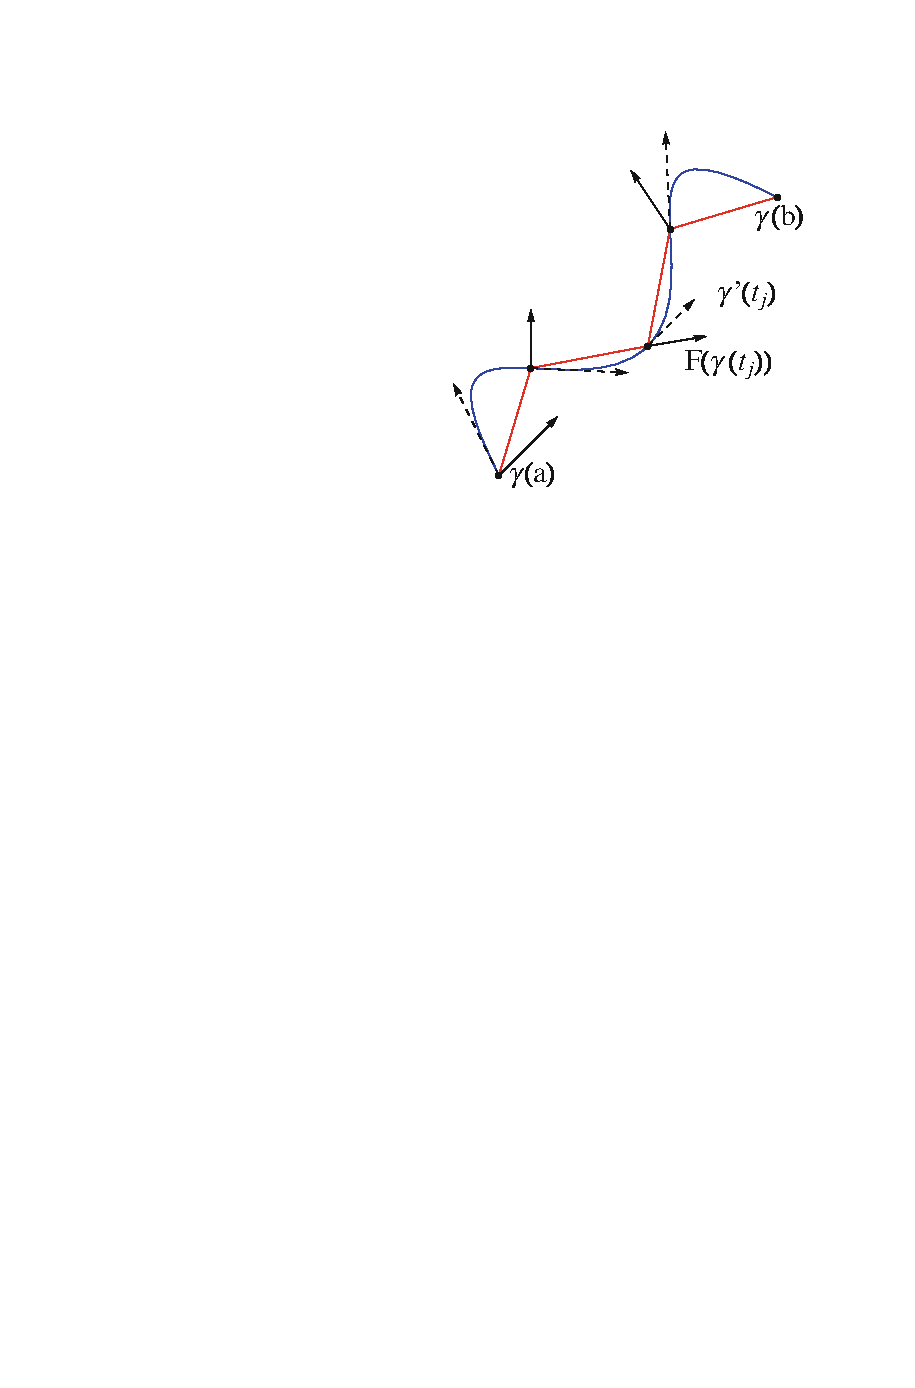
\includegraphics[width=0.6\linewidth]{vector_field_along_path.pdf}
    \caption{حقل متجه على طول مسار}
    \label{fig:enter-label}
\end{figure}
\begin{lemma}

لنفترض أن \( P := \{a = t_1 < t_2 < \cdots < t_k = b\} \) هو تقسيم للفترة [a, b]. لأي دالة مستمرة \( f : [a, b] \to \mathbb{R} \) ولكل اختيار \( u_j \in [t_j, t_{j+1}] \), لدينا:
\[ \lim_{ \|P\| \to 0 } \sum (t_{j+1} - t_j) \cdot f(u_j) = \int_a^b f(t) \, dt. \]

\end{lemma}

\begin{demonstration}

وفقًا لنظرية هاين-كانتور, فإن \( f \) مستمرة بانتظام, مما يعني أنه لكل \( \epsilon > 0 \) يمكن العثور على \( \delta > 0 \) بحيث أن \( |f(s) - f(t)| \leq \epsilon \) عندما يكون \( s \), \( t \in [a, b] \) و \( |s - t| \leq \delta \). لننظر الآن في تقسيم \( P = \{a = t_1 < t_2 < \cdots < t_k = b\} \) بحيث \( 0 < \|P\| < \delta \). إذن:

\[ \left| \sum_{j=1}^{k-1} (t_{j+1} - t_j) \cdot f(u_j) - \int_a^b f(t) \, dt \right| \leq \epsilon (b - a). \]

نظرًا لأن التقسيمات تصبح أدق وأدق, فإن مجموع ريمان يقترب من التكامل المحدد, وبالتالي:

\[ \lim_{\|P\| \to 0} \sum_{j=1}^{k-1} (t_{j+1} - t_j) \cdot f(u_j) = \int_a^b f(t) \, dt. \]
\begin{eqnarray*}
\left| \sum_{j=1}^{k-1} (t_{j+1} - t_j) \cdot f(u_j) - \int_a^b f(t) \, dt \right|
&=& \left| \sum_{j=1}^{k-1} (t_{j+1} - t_j) \cdot f(u_j) - \sum_{j=1}^{k-1} \int_{t_j}^{t_{j+1}} f(t) \, dt \right| \\
&\leq& \sum_{j=1}^{k-1} \left| (t_{j+1} - t_j) \cdot f(u_j) - \int_{t_j}^{t_{j+1}} f(t) \, dt \right| \\
 &\leq& \sum_{j=1}^{k-1} \int_{t_j}^{t_{j+1}} \left| f(u_j) - f(t) \right| dt\\
 \leq \epsilon \sum_{j=1}^{k-1} (t_{j+1} - t_j) = \epsilon (b - a).
 \end{eqnarray*}
وبما أن \( \epsilon \) صغيرة بشكل تعسفي, فإن النتيجة تتبع.

\end{demonstration}

تُظهر التوطئة والمناقشة السابقة لها أن العمل المنجز بواسطة مجال القوة \( F \) على جسيم أثناء حركته على طول \( \gamma \) هو
\[ \int_a^b \langle F(\gamma(t)), \gamma'(t) \rangle \, dt. \]

هذا النوع من التكامل, المعروف بالتكامل الخطي, يظهر كثيرًا في الفصول التالية, ولذلك نقدم تعريفًا رسميًا.

\begin{definition}
لنفترض أن \( F : U \subset \mathbb{R}^n \to \mathbb{R}^n \) هو حقل متجهات مستمر وأن \( \gamma \) هو مسار من الفئة \( C^1 \) من قطعة إلى قطعة في \( U \). يُعطى التكامل الخطي لـ \( F \) على طول \( \gamma \) بواسطة
\[ 
\int_\gamma F := \int_a^b \langle F(\gamma(t)), \gamma'(t) \rangle \, dt. 
\]
\end{definition}


لنعتبر دالة متجهة \(F : U \subset \mathbb{R}^n \to \mathbb{R}^n\), حيث \(U\) هي مجموعة مفتوحة. إذا كانت \(\alpha : [a, b] \to U\) مسارًا منتظمًا بحيث أن مشتقها \(\dot{\alpha}\) موجود ومستمر على \([a, b]\), فإننا نعرف التكامل الخطي لـ\(F\) على \(\alpha\) كما يلي:
\[ \int_\alpha F \cdot d\alpha = \int_a^b F(\alpha(t)) \cdot \dot{\alpha}(t) \, dt. \]

الذي يمثل الشغل الذي تقوم به القوة \(F\) في نقل جسم على طول المسار \(\alpha\).


\section{ تغييرات المعلمة}

في بعض الأحيان, يكون من المفيد إعادة صياغة تكامل خطي باستخدام تغيير في المعلمة. لنفرض أن \(\beta : [c, d] \to [a, b]\) دالة قابلة للتفاضل من الدرجة الأولى وتحقق \(\beta(c) = a\) و \(\beta(d) = b\). إذا كان لدينا مسار منتظم \(\alpha : [a, b] \to \mathbb{R}^n\) فإننا نستطيع تعريف مسار جديد \(\gamma : [c, d] \to \mathbb{R}^n\) بواسطة \(\gamma(t) = \alpha(\beta(t))\). عندها يكون:
\[ \int_\gamma F \cdot d\gamma = \int_c^d F(\gamma(t)) \cdot \dot{\gamma}(t) \, dt = \int_c^d F(\alpha(\beta(t))) \cdot (\alpha'(\beta(t)) \beta'(t)) \, dt. \]

يعتمد التكامل الخطي \( \int_\gamma F \) على حقل المتجهات \( F \) وكذلك على المسار \( \gamma \). في هذا القسم, نخطط لتحليل ما يحدث عند استبدال \( \gamma \) بمسار آخر له نفس الأثر.

\begin{definition}
    
لنفترض أن \( \alpha : [a, b] \to \mathbb{R}^n \) و \( \beta : [c, d] \to \mathbb{R}^n \) هما مساران. نقول أن \( \alpha \) و \( \beta \) متكافئان, ونكتب \( \alpha \sim \beta \), إذا كان هناك دالة \( \varphi : [a, b] \to [c, d] \) من الفئة \( C^1 \), بحيث أن \( \varphi([a, b]) = [c, d] \), \( \varphi'(t) > 0 \) لكل \( t \in [a, b] \) و \( \alpha = \beta \circ \varphi \) (انظر الشكل 2.2).
\end{definition}

بواسطة نظرية القيمة المتوسطة, فإن الشروط على \( \varphi \) في هذا التعريف تضمن أن \( \varphi \) تزايدية بدقة, ومن ثم تكون شاملة, وأن \( c = \varphi(a) \) و \( d = \varphi(b) \). يتبع ذلك أن \( \alpha \sim \beta \) يعني \( \beta \sim \alpha \). في الواقع, \( \beta = \alpha \circ \varphi^{-1} \), و \( \varphi^{-1} \) لها الخصائص اللازمة للتكافؤ.

عادةً ما يشار إلى النتيجة التالية باسم قاعدة السلسلة أو نظرية الدالة المركبة. 

\begin{theoreme}
لنفترض أن \( U \) و \( V \) مجموعات مفتوحة من \( \mathbb{R}^n \) و \( \mathbb{R}^m \) على التوالي. إذا كانت الدالتان \( F : U \to V \) و \( G : V \to \mathbb{R}^p \) قابلتين للتفاضل عند \( a \in U \) و \( F(a) \in V \) على التوالي, فإن تركيبتهما \( H = G \circ F \) قابلة للتفاضل عند \( a \), و
\[ dH(a) = dG(F(a)) \circ dF(a), \]
أو, بعبارات مصفوفاتهما المرتبطة,
\[ H'(a) = G'(F(a)) \cdot F'(a). \]
علاوة على ذلك, إذا كانت \( F \) و \( G \) من الفئة \( C^q \, 1 \leq q \leq \infty\) على مجالات تعريفهما الخاصة, فإن \( H \) أيضًا من الفئة \( C^q \) على \( U \).
\end{theoreme}

نلاحظ أن فرضية قاعدة السلسلة تتضمن دوال معرفة على مجموعات مفتوحة. ومع ذلك, عندما تكون الدالة الأولى معرفة على فترة مغلقة $[a, b]$, فإن نوعًا آخر من النتيجة يكون صحيحًا أيضًا.

\begin{figure}
    \centering
    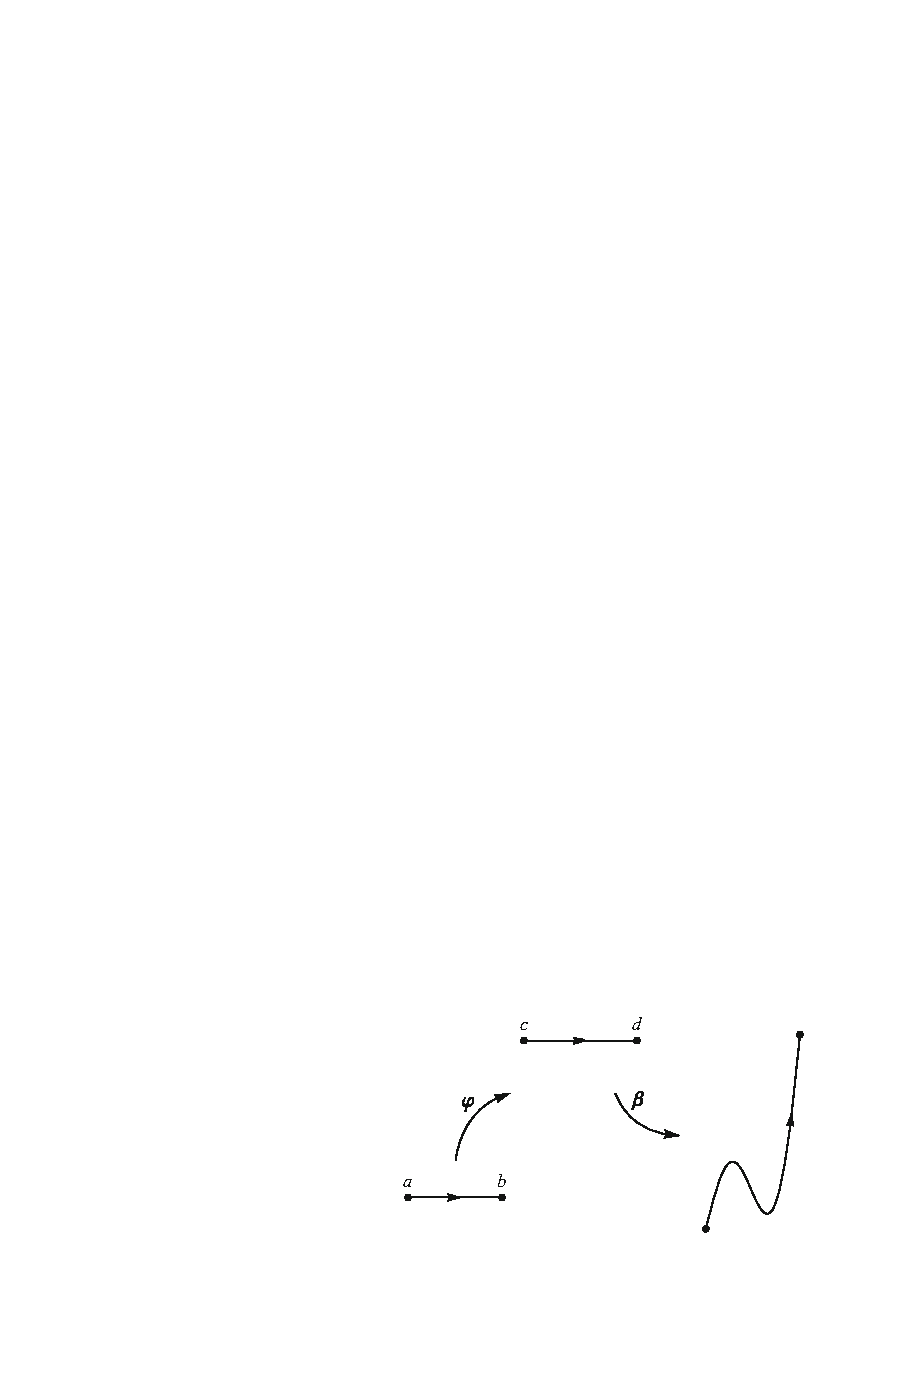
\includegraphics[width=0.75\linewidth]{equivalent path.pdf}
    \caption{مسارات متكافئة}
    \label{fig:enter-label}
\end{figure}

\begin{lemma}
لنفترض أن \( V \) مجموعة مفتوحة من \( \mathbb{R}^m \), و \( \gamma : [a, b] \to V \) مسار له مشتق عند كل نقطة من $[a, b]$, ولنفرض أن \( G : V \to \mathbb{R}^m \) قابل للتفاضل عند كل نقطة من \( \gamma([a, b]) \). إذن \( G \circ \gamma : [a, b] \to \mathbb{R}^m \) له مشتق عند كل نقطة من $[a, b]$ و
\[ (G \circ \gamma)'(t) = G'(\gamma(t)) \cdot \gamma'(t), \]
لكل \( t \in [a, b] \). هنا, تُفهم المشتقات عند \( t = a \) و \( t = b \) كمشتقات من اليمين ومن اليسار على التوالي. علاوة على ذلك, إذا كانت \( \gamma \) من الفئة \( C^q \) على $[a, b]$ و \( G \) من الفئة \( C^q \) على المجموعة المفتوحة \( V \), فإن \( G \circ \gamma \) تكون أيضًا من الفئة \( C^q \) على $[a, b]$.
\end{lemma}

\begin{demonstration}
    
نكتب \( \gamma(t) = (\gamma_1(t), \ldots, \gamma_m(t)) \), حيث \( \gamma_j : [a, b] \to \mathbb{R} \) لها مشتق على $[a, b]$ لكل \( j = 1, \codes, n \) (أو من الفئة \( C^q \) على $[a, b]$ على التوالي).

من المعروف أن \( \gamma_j \) يمكن تمديدها إلى \( \tilde{\gamma}_j : \mathbb{R} \to \mathbb{R} \) مع مشتق عند كل نقطة من \( \mathbb{R} \) (أو من الفئة \( C^q \) على \( \mathbb{R} \) على التوالي). نأخذ \( \tilde{\gamma} = (\tilde{\gamma}_1, \codes, \tilde{\gamma}_m) : \mathbb{R} \to \mathbb{R}^m \). الآن نعرّف \( U = (\tilde{\gamma})^{-1}(V) \). نظرًا لأن \( \tilde{\gamma} \) مستمرة على \( \mathbb{R} \), فإن \( U \) هي مجموعة مفتوحة من \( \mathbb{R} \) تحتوي على [a, b]. علاوة على ذلك, لدينا \( \tilde{\gamma} : U \to V \) و \( G : V \to \mathbb{R}^m \) مع \( \tilde{\gamma} \) و \( G \) قابلتين للتفاضل (على التوالي من الفئة \( C^q \)) على مجالات تعريفهما الخاصة. من قاعدة السلسلة نحصل على النتيجة.
\end{demonstration}

نفس الحجة تثبت بوضوح التباين التالي لقاعدة السلسلة.

\begin{lemma}
    
لنفترض أن \( \alpha : [a, b] \to \mathbb{R} \) قابلة للتفاضل عند كل نقطة من $[a, b]$ وأن \( \beta : [c, d] \to \mathbb{R}^m \) مسار له مشتق عند كل نقطة من $[c, d]$ مع \( \alpha([a, b]) \subset [c, d] \). إذن \( \beta \circ \alpha : [a, b] \to \mathbb{R}^m \) لها مشتق عند كل نقطة من $[a, b]$ و
\[ (\beta \circ \alpha)'(t) = \beta'(\alpha(t)) \cdot \alpha'(t), \]
لكل \( t \in [a, b] \). علاوة على ذلك, إذا كانت \( \alpha \) من الفئة \( C^q \) على $[a, b]$ و \( \beta \) من الفئة \( C^q \) على $[c, d]$, فإن \( \beta \circ \alpha \) تكون أيضًا من الفئة \( C^q \) على $[a, b]$.
\end{lemma}

\begin{lemma}
إذا كان \( \alpha \) و \( \beta \) مساران متكافئان وكان أحدهما, على سبيل المثال \( \beta \), من الفئة \( C^1 \) من قطعة إلى قطعة, فإن \( \alpha \) أيضًا من الفئة \( C^1 \) من قطعة إلى قطعة و \( L(\alpha) = L(\beta) \).
\end{lemma}

\begin{demonstration}
نكتب \( \alpha = \beta \circ \varphi \), حيث أن \( \varphi \) كما في التعريف السابق ولنفرض أن \( Q = \{c = u_1 < \cdots < u_k = d\} \) تقسيم للفترة $[c, d]$ بحيث أن \( \beta|_{[u_j, u_{j+1}]} \) من الفئة \( C^1 \) على $[u_j, u_{j+1}]$.

إذا أخذنا \( t_j := \varphi^{-1}(u_j) \), فإن \( P = \{a = t_1 < \cdots < t_k = b\} \) هو تقسيم للفترة $[a, b]$.

نظرًا لأن \( \alpha|_{[t_j, t_{j+1}]} = (\beta \circ \varphi)|_{[t_j, t_{j+1}]} = (\beta|_{[u_j, u_{j+1}]}) \circ \varphi|_{[t_j, t_{j+1}]} \) هو تركيب دالتين من الفئة \( C^1 \) (على الفترات المغلقة), فإنه يكون نفسه من الفئة \( C^1 \) على $[t_j, t_{j+1}]$, وبالتالي يكون \( \alpha \) من الفئة \( C^1 \) من قطعة إلى قطعة. الآن,
\[ L(\beta) = \int_{c=\varphi(a)}^{d=\varphi(b)} \|\beta'(u)\| \, du = \sum_{j=1}^{k-1} \int_{u_j}^{u_{j+1}} \|\beta'(u)\| \, du. \]

لكل \( 1 \leq j \leq k - 1 \) يمكننا تطبيق تغيير المتغير \( u = \varphi(t) \) للحصول على

\begin{eqnarray*}
    \int_{u_j}^{u_{j+1}} \| \beta'(u) \| du &=&  \int_{t_j}^{t_{j+1}} \| \beta'(\varphi(t)) \|\varphi'(t) dt
    \\
    &=&  \int_{t_j}^{t_{j+1}} \| \beta'(\varphi(t)) \varphi'(t)\| dt = \int_{t_j}^{t_{j+1}} \| (\beta \circ \varphi)'\| dt
    \\
    \int_{t_j}^{t_{j+1}} \| \alpha'(t)\| dt
\end{eqnarray*}

بالجمع لجميع القيم \( 1 \leq j \leq k - 1 \), نستنتج أن
\[ 
L(\beta) = \int_a^b \|\alpha'(t)\| \, dt = L(\alpha). 
\]

\end{demonstration}

\begin{lemma}
لنفترض أن \( \omega \) هي 1-form مستمرة على \( U \), وأن \( \alpha \) و \( \beta \) مساران من الفئة \( C^1 \) من قطعة إلى قطعة في \( U \) بحيث \( \alpha \sim \beta \). إذن
\[ \int_\alpha \omega = \int_\beta \omega. \]
\end{lemma}

\begin{demonstration}
    
دعنا نفترض أولاً أن \( \alpha \) و \( \beta \) مساران من الفئة \( C^1 \). ثم, باستخدام نفس التدوين كما في التمهيدية السابقة, لدينا

\begin{eqnarray*}
    \int_{\beta} \omega &=&  \int_{\varphi(a)}^{\varphi(b)} \omega(\beta(u)) (\beta'(u)) du
    \\
    &=&  \int_{a}^b  \omega(\beta(\varphi(t))) (\beta'(\varphi(t))) \varphi'(t) dt
    \\
    \int_{a}^b  \omega(\beta(\varphi(t))) (\beta \circ \varphi(t)) dt
    \\
    \int_{a}^b  \omega(\alpha(t)) (\alpha'(t)) dt = \int_{\alpha} \omega.
\end{eqnarray*}

Here is the translation of the provided text into Arabic:

---

مرة أخرى نستخدم نظرية قاعدة السلسلة لامتدادات \( \beta \) و \( \phi \) إلى خط الأعداد الحقيقي بأكمله. في الحالة العامة, نعتبر تقسيم
\[ P := \{a = t_1 < t_2 < \cdots < t_k = b\} \]
للفترة $[a, b]$ حيث تكون \( \beta \) من الفئة \( C^1 \) على كل فترة فرعية $[u_j, u_{j+1}] = [\phi(t_j), \phi(t_{j+1})]$. إذن \( \alpha = \beta \circ \phi \) هي أيضًا من الفئة \( C^1 \) على كل فترة فرعية $[t_j, t_{j+1}]$. ولذلك لدينا من أعلاه أن
\[ \int_{\beta_j} \omega = \int_{\alpha_j} \omega, \]
حيث أن \( \beta_j = \beta|_{[u_j, u_{j+1}]} \) و \( \alpha_j = \alpha|_{[t_j, t_{j+1}]} \). بجمع هذه الهوية لجميع القيم من \( j \) من 1 إلى \( k - 1 \), نحصل على
\[ \int_\beta \omega = \int_\alpha \omega. \]
\end{demonstration}

\begin{figure}
    \centering
    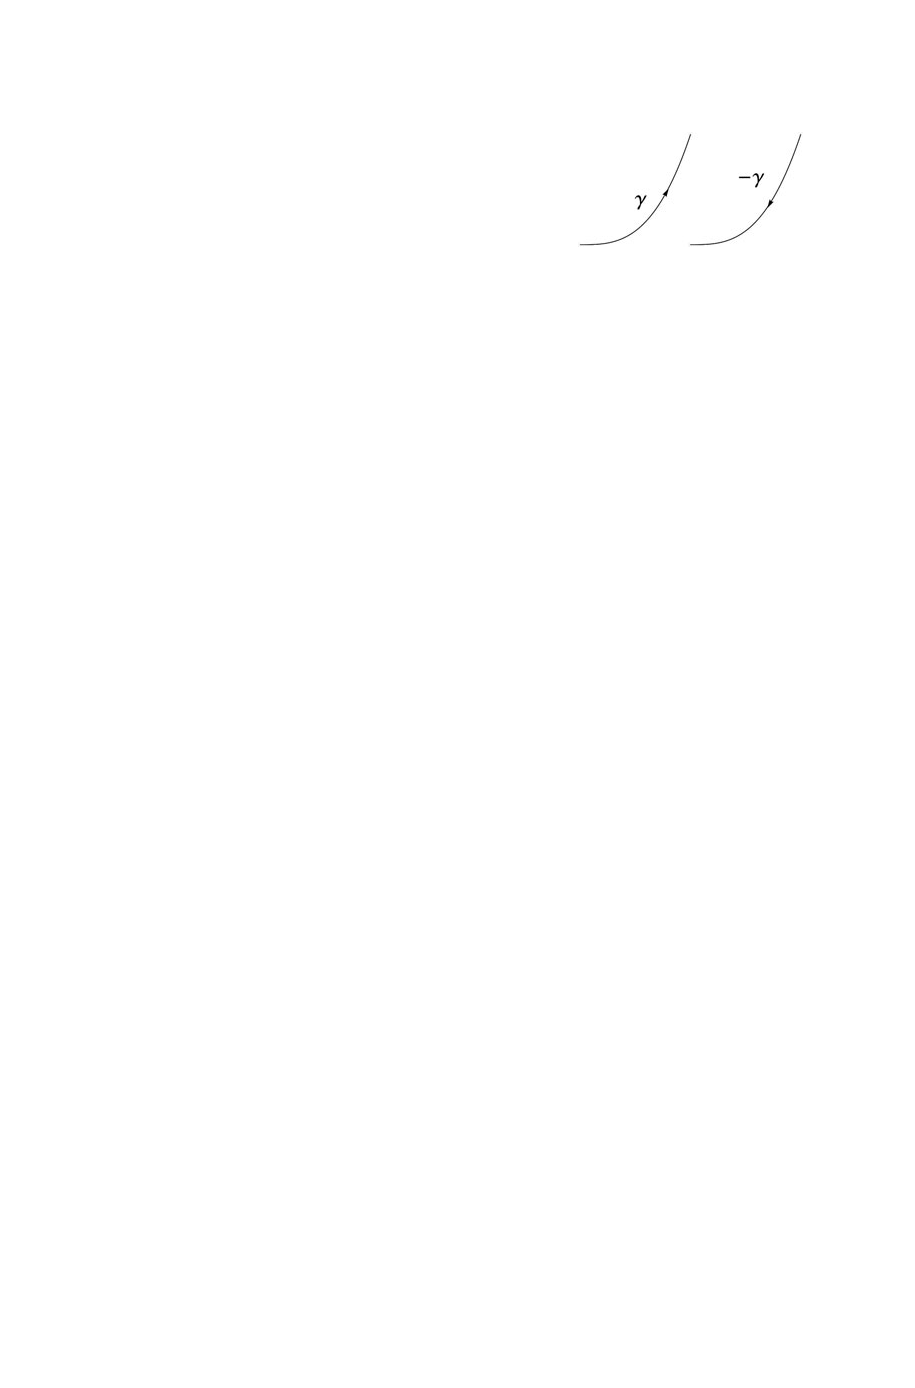
\includegraphics[width=0.5\linewidth]{opposit paths.pdf}
    \caption{$\gamma$ و  $-\gamma$ مسارين متعاكسين}
    \label{fig:enter-label}
\end{figure}

\begin{definition}
لنفترض أن \( \gamma : [a, b] \to \mathbb{R}^n \) هو مسار من الفئة \( C^1 \) من قطعة إلى قطعة. يتم تعريف المسار المعاكس (الشكل 2.3) بواسطة \( (-\gamma) : [−b, −a] \to \mathbb{R}^n \), بحيث \( (-\gamma)(t) := \gamma(−t) \).
\end{definition}

المسار المعاكس \( -\gamma \) يتحرك على طول \( \gamma([a, b]) \) في الاتجاه المعاكس لذلك الذي يعطيه المسار \( \gamma \). النقطة الابتدائية للمسار \( -\gamma \) هي النقطة النهائية للمسار \( \gamma \) والعكس بالعكس. سيلاحظ القارئ الفرق بين \( (-\gamma)(t) \) و \( -(\gamma(t)) \).

\begin{definition}
لنفترض أن \( \alpha : [a, b] \to \mathbb{R}^n \) و \( \beta : [c, d] \to \mathbb{R}^n \) هما مساران من الفئة \( C^1 \) من قطعة إلى قطعة بحيث \( \alpha(b) = \beta(c) \). نعني باتحاد المسارات \( \alpha \) و \( \beta \), المشار إليه بـ \( \alpha \cup \beta \), أي مسار من الفئة \( C^1 \) من قطعة إلى قطعة \( \gamma : [e, f] \to \mathbb{R}^n \) مع الخاصية أنه لبعض \( e < r < f \),
\[ \gamma|_{[e, r]} \sim \alpha \] و \[ \gamma|_{[r, f]} \sim \beta. \]
\end{definition}

من الواضح أن أثر \( \alpha \cup \beta \) هو \( \alpha([a, b]) \cup \beta([c, d]) \) و \( \alpha \cup \beta \) يتكون من تتبع \( \alpha \) أولاً ثم \( \beta \). مثل هذا الاتحاد من المسارات موجود دائمًا, ومثال ملموس يُعطى بواسطة \( \gamma : [0, 1] \to \mathbb{R}^n \), حيث
\[ \gamma(t) = \begin{cases} 
\alpha\left(\frac{2t(b - a) + a}{2}\right), & \text{إذا كان } 0 \leq t \leq \frac{1}{2}, \\
\beta\left((2t - 1)(d - c) + c\right), & \text{إذا كان } \frac{1}{2} \leq t \leq 1.
\end{cases} \]

**الاقتراح 2.4.3.**
لنفترض أن \( \omega \) هي 1-form مستمرة على مجموعة مفتوحة \( U \) من \( \mathbb{R}^n \) وأن \( \alpha \) و \( \beta \) و \( \gamma \) هي ثلاثة مسارات من الفئة \( C^1 \) من قطعة إلى قطعة في \( U \) مع نقطة النهاية للمسار \( \alpha \) تتطابق مع النقطة الابتدائية للمسار \( \beta \). إذن:
1. \( \int_{-\gamma} \omega = -\int_\gamma \omega \).
2. \( \int_{\alpha \cup \beta} \omega = \int_\alpha \omega + \int_\beta \omega \).

**الدليل.**
بما أن \( (-\gamma)'(t) = -\gamma'(-t) \), فإن التبديل \( u = -t \) يعطي
\[ \int_{-\gamma} \omega = \int_{-a}^{-b} \omega(\gamma(-t)) \cdot (-\gamma'(-t)) \, dt = \int_{b}^{a} -\omega(\gamma(u)) \cdot \gamma'(u) \, du = -\int_\gamma \omega. \]

أيضًا,
\[ \int_{\alpha \cup \beta} \omega = \int_e^r \omega(\gamma(t)) \cdot \gamma'(t) \, dt + \int_r^f \omega(\gamma(t)) \cdot \gamma'(t) \, dt = \int_\alpha \omega + \int_\beta \omega. \]


\section{ الحقول المحافظة: الأشكال التفاضلية التامة}


نبدأ هذا القسم بمثال على حقل متجهات يكون فيه التكامل الخطي على مسارين مختلفين من (0, 0) إلى (1, 1) هو نفسه.

\begin{exemple}
لنفترض أن \( F : \math{R}^2 \to \math{R}^2 \) هو حقل المتجهات المحدد بواسطة \( F(x, y) = (x, y) \) ولنعتبر المسارين (الشكل 2.4)
\[ \gamma_1 : [0, 1] \to \math{R}^2 \] و\[ \gamma_2 : [0, 1] \to \math{R}^2 \] المعرفين بواسطة \[ \gamma_1(t) = (t, t) \] و\[ \gamma_2(t) = (t, t^2) \]. إذن
\[ \int_{\gamma_1} F = \int_0^1 \langle (t, t), (1, 1) \rangle \, dt = \int_0^1 (t + t) \, dt = 1. \]
وأيضًا
\[ \int_{\gamma_2} F = \int_0^1 \langle (t, t^2), (1, 2t) \rangle \, dt = \int_0^1 (t + 2t^3) \, dt = 1. \]
\end{exemple}

\begin{figure}
    \centering
    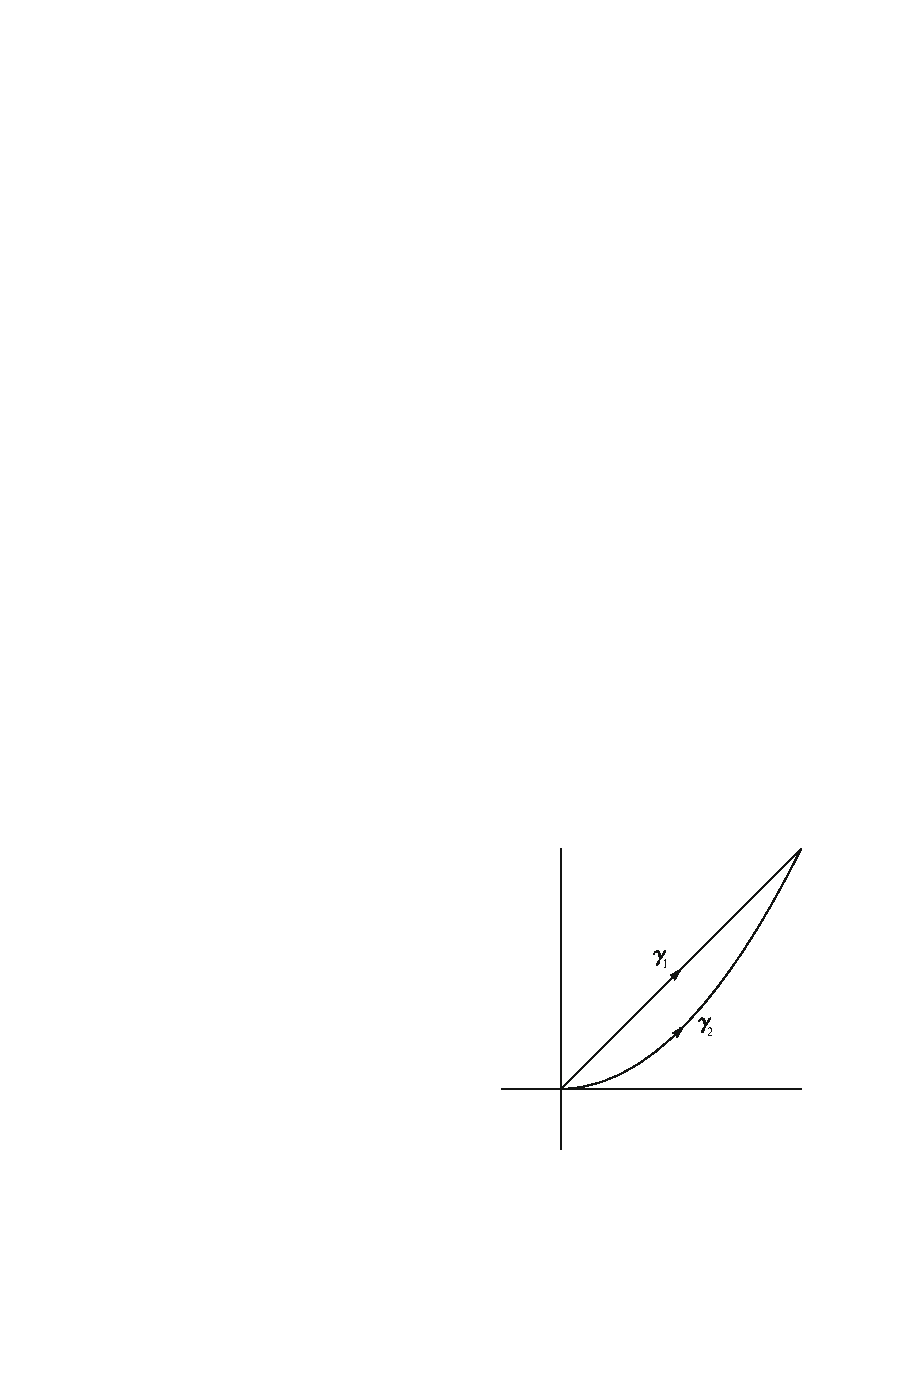
\includegraphics[width=0.5\linewidth]{path example.pdf}
    \caption{}
    \label{fig:enter-label}
\end{figure}

حقيقة أن التكاملين الخطيين هنا يأخذان نفس القيمة ليست مفاجئة إذا تذكرنا أن التكامل الخطي يمثل العمل المنجز بواسطة حقل قوة في تحريك جسيم على طول مسار, ومن المعروف في الفيزياء أنه تحت تأثير حقل الجاذبية, العمل المنجز لنقل جسم بين نقطتين مختلفتين يعتمد فقط على فرق طاقات الجهد عند هاتين النقطتين, وبالتالي يكون مستقلًا عن المسار المتخذ (انظر المثال 2.5.4). مثالنا التالي, حقل متجهات يكون فيه التكامل الخطي على مسارين مختلفين من (0, 0) إلى (1, 1) مختلفًا, يوضح أن هذا السلوك ليس عالميًا.

\begin{exemple}
    
**المثال 2.5.2.** 
لنفترض أن \( \gamma_1 \) و \( \gamma_2 \) هما المساران المعطيان في المثال السابق ولكن دعنا نعتبر بدلاً من ذلك حقل المتجهات
\[ F(x, y) = (-y + 3, x - 1). \]
إذن
\[ \int_{\gamma_1} F = \int_0^1 \langle (-t + 3, t - 1), (1, 1) \rangle \, dt = \int_0^1 (-t + 3 + t - 1) \, dt = \int_0^1 (2) \, dt = 2. \]

وأيضًا
\begin{eqnarray*}
     \int_{\gamma_2} F &=& \int_0^1 \langle (-t^2 + 3, t - 1), (1, 2t) \rangle \,dt 
     \\
     &=& \int_0^1 (-t^2 + 3 + 2t(t - 1)) \, dt = \int_0^1 (-t^2 + 3 + 2t^2 - 2t) \, dt 
     \\
     &=& \int_0^1 (t^2 - 2t + 3) \, dt.
\end{eqnarray*}
لحساب هذا التكامل, نلاحظ أن:
\[ \int_0^1 (t^2 - 2t + 3) \, dt = \int_0^1 t^2 \, dt - 2 \int_0^1 t \, dt + \int_0^1 3 \, dt. \]

نحسب هذه التكاملات على التوالي:
\[ \int_0^1 t^2 \, dt = \left[ \frac{t^3}{3} \right]_0^1 = \frac{1}{3}, \]
\[ 2 \int_0^1 t \, dt = 2 \left[ \frac{t^2}{2} \right]_0^1 = 1, \]
\[ \int_0^1 3 \, dt = 3 \left[ t \right]_0^1 = 3. \]

وبالتالي:
\[ \int_0^1 (t^2 - 2t + 3) \, dt = \frac{1}{3} - 1 + 3 = \frac{1}{3} + 2 = \frac{7}{3}. \]

إذن
\[ \int_{\gamma_2} F = \frac{7}{3}. \]
\end{exemple}

هذه الحقيقة تُظهر أن التكامل الخطي يعتمد على المسار المتخذ, وأن هذا السلوك ليس عاما كما كان في المثال السابق.

\begin{definition}
لنفترض أن \( F = (f_1, \ldots, f_n) \) هو حقل متجهات على مجموعة مفتوحة \( U \) من \( \mathbb{R}^n \) مع 1-form المرتبطة \( \omega = f_1 \cdot dx_1 + \cdots + f_n \cdot dx_n \). إذا كانت هناك دالة من الفئة \( C^1 \), \( f : U \subset \mathbb{R}^n \to \mathbb{R} \), بحيث أن \( \nabla f = F \) (أو بشكل مكافئ, \( df = \omega \)) على \( U \), فإن حقل المتجهات \( F \) يُقال إنه محافظ و1-form \( \omega \) يُقال إنها دقيقة. الدالة العددية \( f \) تُسمى دالة الجهد لحقل المتجهات المحافظ \( F \).
\end{definition}

تتمتع الحقول المحافظة بسلوك مشابه لذلك في المثال السابق من حيث أن تكاملاتها الخطية مستقلة عن المسار. هذه نتيجة فورية للنتيجة التالية, التي هي تعميم لنظرية التفاضل الأساسية.

\begin{theoreme}[2.5.1]
لنفترض أن \( g : U \subset \mathbb{R}^n \to \mathbb{R} \) دالة من الفئة \( C^1 \) على مجموعة مفتوحة \( U \) وأن \( \gamma : [a, b] \to U \) مسار من الفئة \( C^1 \) من قطعة إلى قطعة. إذن
\[ \int_\gamma \nabla g = \int_\gamma dg = g(\gamma(b)) - g(\gamma(a)). \]
\end{theoreme}

\begin{demonstration}

بما أن \( dg \) هو 1-form المرتبط بحقل المتجهات \( \nabla g \), فإن المعادلة الأولى تتبع من ملاحظتنا المباشرة التي تسبق القسم السابق بالنسبة للمعادلة الثانية, نأخذ التوسع المعتاد لـ 1-form \( dg \),
\[ dg = \sum_{j=1}^n \frac{\partial g}{\partial x_j} \cdot dx_j, \]
ونطبق قاعدة السلسلة,
\[ \sum_{j=1}^n \frac{\partial g}{\partial x_j} (\gamma(t)) \gamma_j'(t) = (g \circ \gamma)'(t), \]
وهي صالحة لجميع \( t \) ما عدا مجموعة منتهية في $[a, b]$, للحصول على
\[
\int_\gamma dg = \int_a^b \sum_{j=1}^n \frac{\partial g}{\partial x_j} (\gamma(t)) \gamma_j'(t) \, dt = \int_a^b (g \circ \gamma)'(t) \, dt. 
\]
لنفرض أن \( P := \{a = t_1 < \cdots < t_k = b\} \) هو تقسيم بحيث أن \( \gamma|_{[t_i, t_{i+1}]} \) من الفئة \( C^1 \) لكل \( 1 \leq i \leq k - 1 \). تعطي نظرية التفاضل الأساسية
\[ \int_\gamma dg = \sum_{i=1}^{k-1} \int_{t_i}^{t_{i+1}} (g \circ \gamma)'(t) \, dt \]

\[ = \sum_{i=1}^{k-1} (g \circ \gamma)(t_{i+1}) - (g \circ \gamma)(t_i) \]

\[ = g(\gamma(b)) - g(\gamma(a)). \]

\end{demonstration}

لتذكيرنا بالمفاهيم المتعلقة بالمجموعات المتصلة والمجموعات المتصلة بالمسار.

\begin{definition}
لنفترض أن \( C \) هو مجموعة جزئية من \( \mathbb{R}^n \).
\begin{enumerate}
    \item[1.]  يُقال إن \( C \) متصلة إذا لم توجد مجموعتان مفتوحتان \( V \) و \( W \) في \( \mathbb{R}^n \) بحيث:
\begin{itemize}
    \item [أ.] \( C \subset V \cup W \);
    \item [ ب.] \( C \cap V \neq \emptyset \) و \( C \cap W \neq \emptyset \);
    \item [ ج.] \( C \cap V \cap W = \emptyset \).
\end{itemize}   
   بمعنى آخر, تكون المجموعة \( C \) متصلة إذا وفقط إذا كانت المجموعة الفرعية من \( C \) التي تكون مفتوحة ومغلقة في آن واحد هي \( C \) نفسها والمجموعة الفارغة \( \emptyset \).
\item[2.]  يُقال إن \( C \) متصلة بالمسار إذا كان لكل \( x, y \in C \), هناك مسار \( \gamma : [a, b] \to C \) بحيث \( \gamma(a) = x \) و \( \gamma(b) = y \). إذا كان يمكن اختيار المسار ليكون مضلعياً, فإن المجموعة تُسمى متصلة مضلعياً.
\end{enumerate}
\end{definition}

الصورة المستمرة لمجموعة متصلة هي متصلة, مما يعني أن كل مجموعة متصلة بالمسار هي متصلة. بالنسبة لمجموعة مفتوحة من \( \mathbb{R}^n \), فإن العكس أيضًا صحيح, وتتماهى المفاهيم الاثنين.

\begin{theoreme}[النظرية 2.5.2]
   
لنفترض أن \( U \) مجموعة مفتوحة متصلة من \( \mathbb{R}^n \). إذن \( U \) متصلة مضلعياً.
\end{theoreme}

\begin{theoreme}[النظرية 2.5.3]
    
لنفترض أن \( F : U \subset \mathbb{R}^n \to \mathbb{R}^n \) حقل متجهات مستمر على مجموعة مفتوحة \( U \). الشروط التالية متكافئة:
\begin{enumerate}
    \item [1.] \( F \) هو حقل متجهات محافظ.
    \item [2.] إذا كان \( \gamma : [a, b] \to U \subset \mathbb{R}^n \) مسار من الفئة \( C^1 \) من قطعة إلى قطعة ومغلق (أي \( \gamma(a) = \gamma(b) \)), إذن
    \[ \int_\gamma F = 0. \]
    \item [3.] إذا كان \( \gamma_1 \) و \( \gamma_2 \) مسارين من الفئة \( C^1 \) من قطعة إلى قطعة ولهما نفس النقطة الابتدائية والنقطة النهائية, إذن
    \[ 
    \int_{\gamma_1} F = \int_{\gamma_2} F. 
    \]
\end{enumerate}
\end{theoreme}

(1) $\Leftarrow$ (2). وفقًا للفرضية, هناك دالة \( f \) من الفئة \( C^1 \) على \( U \), بحيث \( \nabla f = F \). لنفترض أن \( \gamma : [a, b] \to U \) مسار مغلق من الفئة \( C^1 \) من قطعة إلى قطعة. وفقًا للنظرية 2.5.1,
\[ \int_\gamma F = f(\gamma(b)) - f(\gamma(a)) = 0. \]

(2) $\Leftarrow$ (3). إذا كان \( \gamma_1 \) و \( \gamma_2 \) لهما نفس النقطة الابتدائية والنقطة النهائية, إذن \( \gamma := \gamma_1 \cup (-\gamma_2) \) هو مسار مغلق من الفئة \( C^1 \) من قطعة إلى قطعة في \( U \). بالتالي,
\[ \int_{\gamma_1} F - \int_{\gamma_2} F = \int_\gamma F = 0. \]

(3) $\Leftarrow$ (1). لنفترض أولاً أن \( U \) مجموعة مفتوحة متصلة في \( \mathbb{R}^n \). إذن \( U \) متصلة بالمسار ومتصلة مضلعياً. نثبت نقطة \( x_0 \) في \( U \) ونعرف دالة الجهد \( f : U \subset \mathbb{R}^n \to \mathbb{R} \) كما يلي (الشكل 2.5): لكل \( x \in U \) لنفترض أن \( \gamma_x \) هو مسار مضلعي في \( U \) من \( x_0 \) إلى \( x \) ونحدد
\[ f(x) := \int_{\gamma_x} F. \]
تتضمن فرضية (3) أن \( f(x) \) لا تعتمد على المسار المضلع المختار \( \gamma_x \), وبالتالي يكون التعريف غير ملتبس. لإثبات النتيجة, سنبين أن \( f \) هي دالة من الفئة \( C^1 \) والتي يتطابق تدرجها مع حقل المتجهات \( F \).

لنفترض \( x \in U \), يمكننا إيجاد \( \delta > 0 \) بحيث تكون الكرة المفتوحة \( B(x, \delta) \) المتمركزة عند \( x \) ونصف قطرها \( \delta \) محتواة في \( U \). نلاحظ أنه لكل \( 1 \leq j \leq n \) و \( 0 < |t| < \delta \), إذا كان \( \gamma_x \) هو مسار مضلعي في \( U \) من النقطة \( x_0 \) إلى النقطة \( x \), فإن \( \gamma_x \cup [x, x + t e_j] \) هو مسار مضلعي في \( U \) من \( x_0 \) إلى \( x + t e_j \). لذا
\[ f(x + t e_j) - f(x) = \int_{\gamma_x \cup [x, x + t e_j]} F - \int_{\gamma_x} F = \int_{[x, x + t e_j]} F. \]

لنفترض للبساطة أن \( t > 0 \) ونقوم للبارامترة الجزء الخطي بواسطة \( \gamma(s) = x + s e_j \), \( 0 \leq s \leq t \). نكتب أيضًا \( F \) بمصطلحات الدوال المكونة, \( F = (f_1, \ldots, f_n) \). إذن لكل \( 1 \leq j \leq n \),
\[ f(x + t e_j) - f(x) = \int_0^t \langle F(x + s e_j), e_j \rangle \, ds = \int_0^t f_j(x + s e_j) \, ds. \]

يتبع ذلك أن
\[ \frac{f(x + t e_j) - f(x)}{t} = \frac{1}{t} \int_0^t f_j(x + s e_j) \, ds. \]

نحسب هذه القيم على التوالي:
\[ \frac{f(x + t e_j) - f(x)}{t} = \frac{1}{t} \int_0^t f_j(x + s e_j) \, ds \leq \frac{1}{t} \int_0^t |f_j(x + s e_j) - f_j(x)| \, ds. \]

بما أن كل \( f_j \) هو دالة مستمرة, فإن التعبير أعلاه يميل إلى الصفر مع اقتراب \( t \) من الصفر. نتيجة لذلك,
\[ \frac{\partial f}{\partial x_j}(x) = f_j(x). \]

بالتحديد, \( f \) هي دالة من الفئة \( C^1 \) و \( \nabla f = F \) على \( U \). في الحالة العامة حيث \( U \) غير متصلة, يمكن تطبيق الحجة أعلاه على كل مكون متصل من \( U \) من أجل إنشاء دالة جهد مناسبة.
\end{demonstration}
\begin{figure}
    \centering
    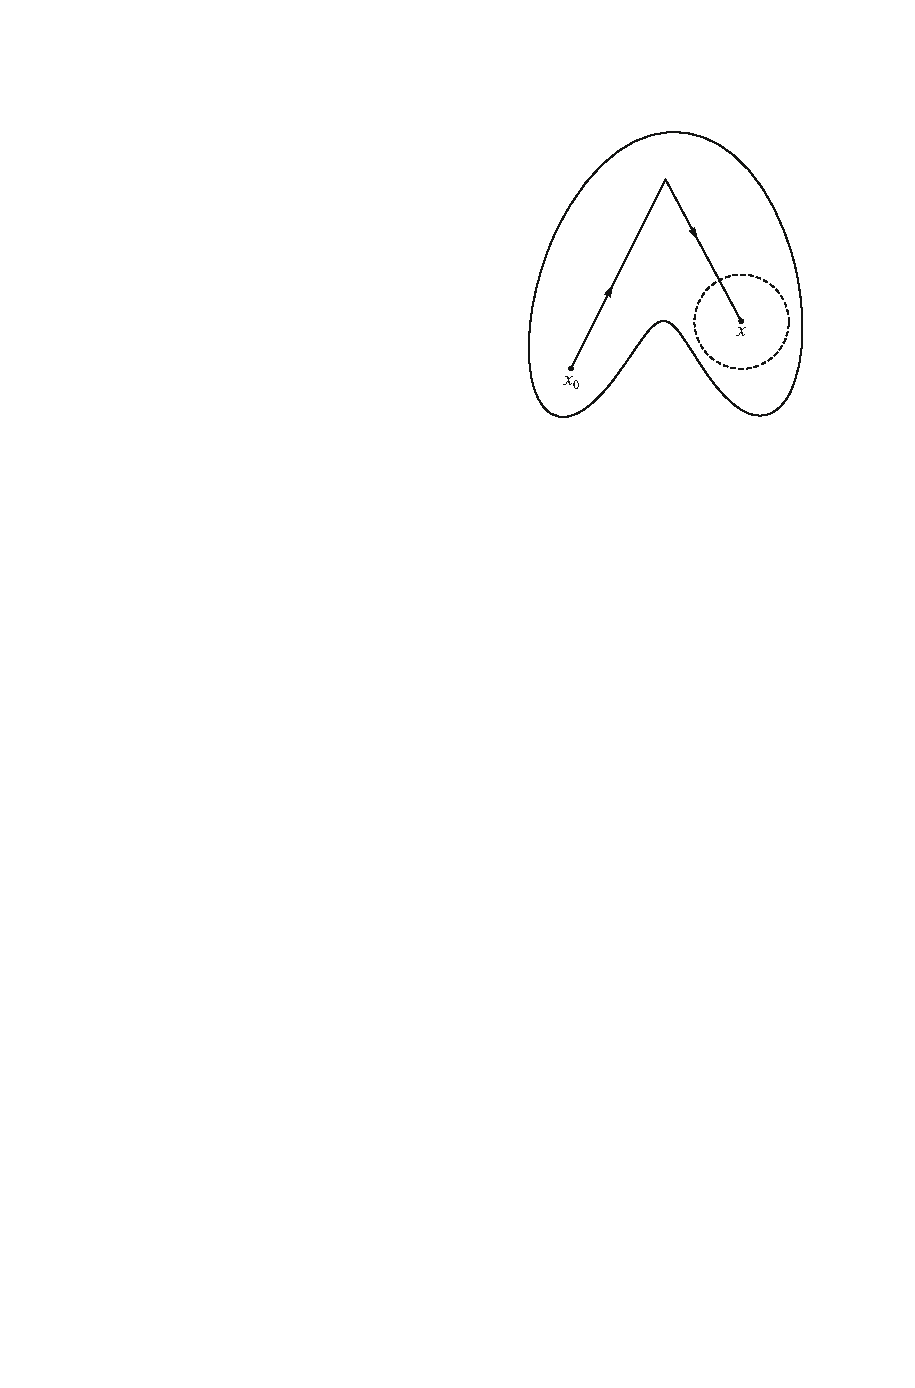
\includegraphics[width=0.5\linewidth]{polygonal_path.pdf}
    \caption{}
    \label{fig:enter-label}
\end{figure}

\begin{definition}
يُقال إن المجموعة المفتوحة \( U \subset \mathbb{R}^n \) نجميّة بالنسبة للنقطة \( a \in U \) إذا كان الجزء \([a, x]\) مُحتوى في \( U \) لكل \( x \in U \).
\end{definition}

نذكر أن المثلث الذي يضم الرؤوس \( a, x, y \) هو المجموعة \(\{\alpha a + \beta x + \gamma y : 0 \leq \alpha, \beta, \gamma \quad\text{ و}\quad \alpha + \beta + \gamma = 1 \}\). عن طريق حدوده, نفهم القوس المضلع المغلق $[a, x] \cup  [x, y] \cup  [y, a]$.

\begin{lemma}
لنفترض أن \( U \) نجميّة بالنسبة للنقطة \( a \in U \). إذا كانت \( y \in B(x, R) \subset U \), فإن المثلث (الشكل 2.6) ذو الرؤوس \( a, x, y \) يكون محتوى في \( U \).
\end{lemma}

\begin{figure}
    \centering
    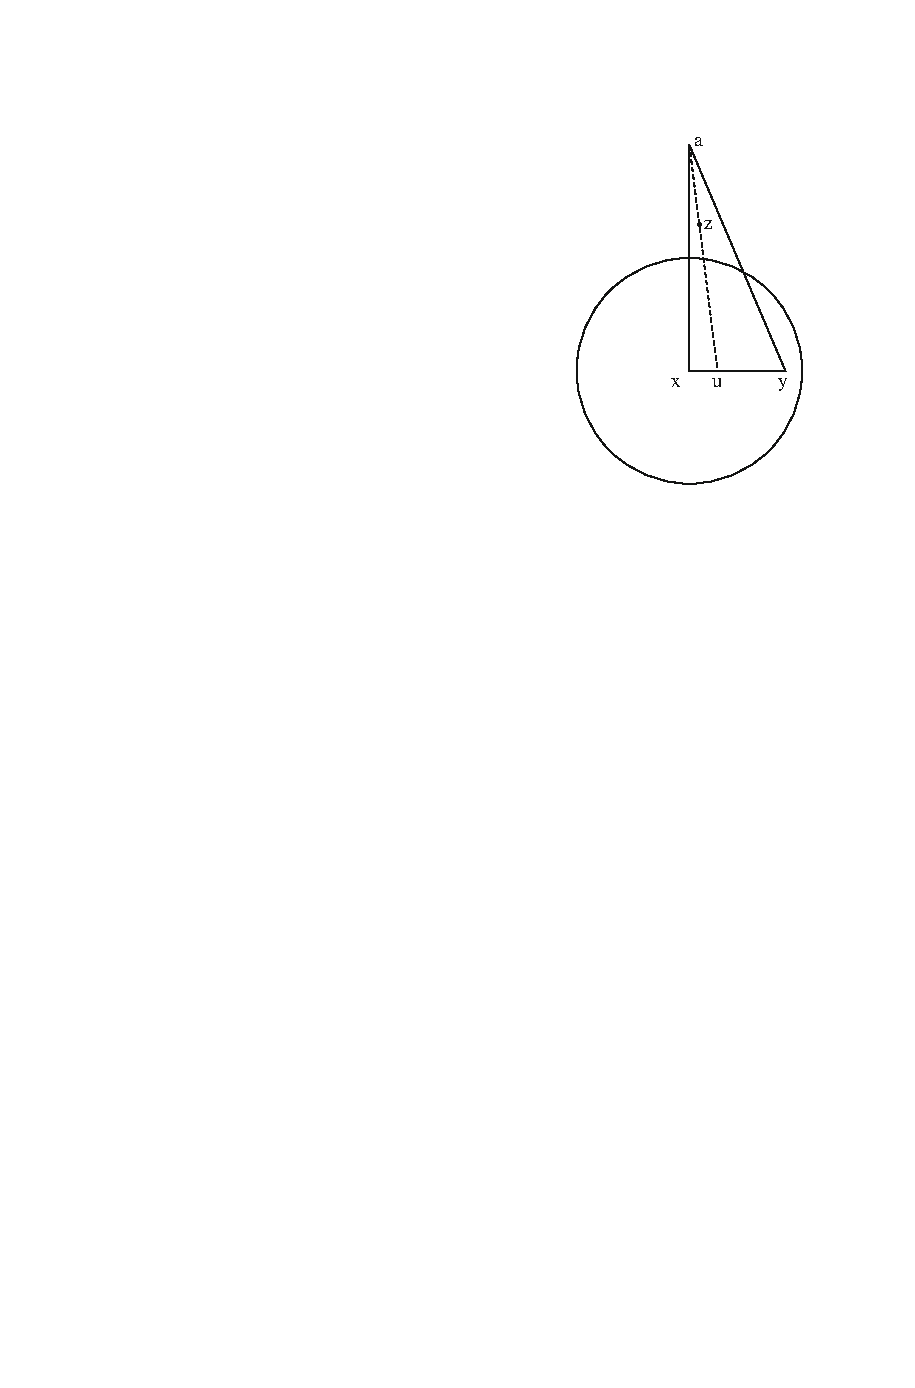
\includegraphics[width=0.5\linewidth]{Triangle_lemma.pdf}
    \caption{}
    \label{fig:enter-label}
\end{figure}

\begin{demonstration}
لنفترض أن \( z = \alpha a + \beta x + \gamma y \) معطى, حيث \( \alpha, \beta, \gamma \geq 0 \) و \(\alpha + \beta + \gamma = 1\). إذا كانت \(\alpha = 1\), فإن \( z = a \in U \). في الحالة الأخرى, نضع
\[ u = \frac{\beta x + \gamma y}{1 - \alpha}. \]
بما أن
\[ \frac{\beta}{1 - \alpha} + \frac{\gamma}{1 - \alpha} = 1, \]
نحصل على أن \( u \in [x, y] \subset B(x, R) \subset U \). أخيرًا, من \( z = \alpha a + (1 - \alpha) u \) نستنتج أن
\[ z \in [a, u] \subset U. \]
\end{demonstration}

\begin{theoreme}
إذا كانت المجموعة المفتوحة \( U \) نجميّة بالنسبة للنقطة \( a \in U \), فإن شروط النظرية 2.5.3 مكافئة لما يلي:
(4) إذا كان \( \gamma \) هو حدود مثلث محتوى في \( U \), إذن
\[ \int_\gamma \omega = 0. \]
\end{theoreme}

\begin{demonstration}
بما أن الشرط (2) يعني بوضوح الشرط (4), يكفي أن نثبت أن الشرط (4) يعني الشرط (1). نفعل ذلك من خلال الحجة أن الدالة \( f \) المعرفة بواسطة
\[ f(x) := \int_{[a, x]} F, \]
هي في الواقع دالة الجهد لحقل المتجهات \( F \). لكل \( x \in U \) نختار \( R_x > 0 \) مع \( B(x, R_x) \subset U \). وفقًا للّمة السابقة, لكل \( 1 \leq j \leq n \) ولكل \( t \in \mathbb{R} \) بحيث \(|t| < R_x \), المثلث ذو الرؤوس \( a, x, و x + t e_j \) يكون محتوى في \( U \). لذا, نستنتج من الشرط (4) أن
\[ f(x + t e_j) - f(x) = \int_{[a, x + t e_j]} F - \int_{[a, x]} F = \int_{[x, x + t e_j]} F. \]

الآن, يستمر الحجة كما في إثبات (3) $\Leftarraw$ (1) في النظرية 2.5.3. 
\end{demonstration}
بالطبع, يمكن تفسير النظرية 2.5.3 أيضًا على أنها وصف لتلك الأشكال التفاضلية من الدرجة الأولى التي تكون دقيقة.

\begin{exemple}
    لنفترض أن
\[ \omega = -\frac{y}{x^2 + y^2} \, dx + \frac{x}{x^2 + y^2} \, dy, \]
وهي 1-form مستمرة في \( U := \mathbb{R}^2 \setminus \{(0, 0)\} \). إذن \( \omega \) ليست دقيقة, نظرًا لأن \( \gamma : [0, 2\pi] \to \mathbb{R}^2 \), \( \gamma(t) := (\cos(t), \sin(t)) \), يحدد مسارًا مغلقًا محتوى في \( U \) لـ
\[ \int_\gamma \omega = 2\pi \neq 0. \]

ومع ذلك, إذا اعتبرنا \( V := \mathbb{R}^2 \setminus \{(0, y) : y \in \mathbb{R}\} \) و \( g : V \to (-\pi, \pi) \) معرّفة بواسطة
\[ g(x, y) := \arctan\left(\frac{y}{x}\right), \]
إذن \( \omega = dg \) على \( V \).
\end{exemple}

وهكذا, فإن حقيقة أن حقل المتجهات محافظ يعتمد ليس فقط على تعبير الحقل بل أيضًا على المنطقة \( U \) التي نتعامل معها. أي أن حقل المتجهات الذي يعترف بدالة جهد في مجموعة مفتوحة معينة قد لا يكون محافظًا في مجموعة أكبر.

\begin{exemple}
(
الحقل الجاذبي محافظ.) 
لنفترض وجود جسيم ذو كتلة \( M \) يقع عند الأصل. قوة الجذب المؤثرة على جسيم ذو كتلة وحدة يقع عند النقطة \( (x, y, z) \in \mathbb{R}^3 \setminus \{(0, 0, 0)\} \) هي
\[ F(x, y, z) = -\frac{GM(x, y, z)}{(x^2 + y^2 + z^2)^{3/2}}, \]
حيث \( G \) هو ثابت الجاذبية. بما أن مقدار القوة هو نفسه في جميع النقاط التي تبعد نفس المسافة عن الأصل, يبدو معقولًا أن نتوقع أن يكون هذا صحيحًا أيضًا بالنسبة لدالة الجهد. وبالتالي, نبحث عن دالة لـ \( r = \sqrt{x^2 + y^2 + z^2} \) التي يكون مشتقها \(-\frac{GM}{r^2}\). مثال على مثل هذه الدالة هو
\[ f(x, y, z) := -\frac{GM}{\sqrt{x^2 + y^2 + z^2}}, \]
ومن السهل التحقق من أن \( \nabla f = F \). أي أن \( f \) هي دالة الجهد للحقل الجاذبي.
\end{exemple}

ينبغي ملاحظة أن ما يسمى بجهد الجاذبية في الفيزياء هو الدالة \( V := -f \). وبالتالي, فإن العمل المنجز بواسطة الحقل لنقل جسيم من النقطة \( A \) إلى النقطة \( B \) يكون مستقلًا عن مسار الجسيم, وقيمته هي الفرق بين الجهود \( V(A) - V(B) \).

\begin{theoreme}
لنفترض أن \( F : U \subset \mathbb{R}^n \to \mathbb{R}^n \) هو حقل متجهات محافظ من الفئة \( C^1 \) على مجموعة مفتوحة \( U \) ونكتب \( F := (f_1, f_2, \cdots, f_n) \). إذن
\[ \frac{\partial f_j}{\partial x_k} (x) = \frac{\partial f_k}{\partial x_j} (x) \]
لكل \( j, k \in \{1, \cdots, n\} \) ولكل \( x \in U \).
\end{theoreme}

\begin{demonstration}
   
وفقًا للفرضية, هناك دالة \( g : U \subset \mathbb{R}^n \to \mathbb{R} \) بحيث \( \nabla g = F \). لذلك, \( f_j = \frac{\partial g}{\partial x_j} \), ويمكننا كتابة
\[ \frac{\partial f_j}{\partial x_k} (x) = \frac{\partial^2 g}{\partial x_k \partial x_j} (x) \]
وبالمثل
\[ \frac{\partial f_k}{\partial x_j} (x) = \frac{\partial^2 g}{\partial x_j \partial x_k} (x) \]
لكل \( x \in U \). بما أن \( F \) هو دالة من الفئة \( C^1 \) على \( U \), فإنه يتبع أن \( g \) من الفئة \( C^2 \), ونظرية Schwarz المتعلقة بتناظر المشتقات الجزئية من الدرجة الثانية تعطينا النتيجة.
\end{demonstration}

على وجه الخصوص, إذا كان \( F = (P, Q) \) حقل متجهات محافظ على \( U \subset \mathbb{R}^2 \) من الفئة \( C^1 \), فإن لكل \( (x, y) \in U \),
\[ \frac{\partial Q}{\partial x} (x, y) = \frac{\partial P}{\partial y} (x, y). \]

يتبع أيضًا من التعريف 1.2.11 والنظرية 2.5.5 أن كل حقل متجهات محافظ \( F = (f_1, f_2, f_3) \) على المجموعة المفتوحة \( U \subset \mathbb{R}^3 \) من الفئة \( C^1 \) يحقق
\[ \text{Curl} \, F (x, y, z) = \left( \frac{\partial f_3}{\partial y} - \frac{\partial f_2}{\partial z}, \frac{\partial f_1}{\partial z} - \frac{\partial f_3}{\partial x}, \frac{\partial f_2}{\partial x} - \frac{\partial f_1}{\partial y} \right) = 0 \]
لكل \( (x, y, z) \in U \).
\\
في المثال 2.5.3 أثبتنا أن حقل المتجهات
\[ F = (P, Q) : U \subset \mathbb{R}^2 \to \mathbb{R}^2 \]
المعرف على \( U = \mathbb{R}^2 \setminus \{(0, 0)\} \) بواسطة
\[ P(x, y) = - \frac{y}{x^2 + y^2}, Q(x, y) = \frac{x}{x^2 + y^2} \]
ليس محافظًا. ومع ذلك,
\[ \frac{\partial Q}{\partial x} (x, y) = \frac{\partial P}{\partial y} (x, y) = \frac{y^2 - x^2}{(x^2 + y^2)^2}. \]

لذا, فإن الشرط في النظرية 2.5.5 ليس كافيًا, بشكل عام, لكي يكون حقل المتجهات محافظًا. ومع ذلك, إذا فرضنا شروطًا هندسية معينة على المجال \( U \), فإن الشرط في النظرية 2.5.5 يكون كافيًا, كما تظهر النظرية التالية. قبل عرض النتيجة, نحتاج إلى تذكر الحقيقة التالية حول مشتق التكامل (يُسمى أيضًا المشتق البارامتري).

\begin{lemma}
    
لنفترض أن \( f : [a, b] \times [c, d] \to \mathbb{R} \) هي دالة من الفئة \( C^1 \) وأن \( g : [a, b] \to \mathbb{R} \) معرّفة بواسطة
\[ g(x) = \int_c^d f(x, t) \, dt. \]
إذن \( g \) هي دالة من الفئة \( C^1 \) على \([a, b]\) و
\[ g'(x) = \int_c^d \frac{\partial f}{\partial x} (x, t) \, dt \]
لكل \( x \in [a, b] \).
\end{lemma}

\begin{theoreme}[مبرهنة بوانكاريه]
    

لنفترض أن \( F : U \subset \mathbb{R}^n \to \mathbb{R}^n \) هو حقل متجهات من الفئة \( C^1 \), \( F := (f_1, f_2, \cdots, f_n) \), على مجموعة مفتوحة \( U \) نجميّة بالنسبة للنقطة \( a \). إذا كان
\[ \frac{\partial f_j}{\partial x_k} (x) = \frac{\partial f_k}{\partial x_j} (x) \]
لكل اختيار للفهارس \( 1 \leq j, k \leq n \) ولكل \( x \in U \), إذن \( F \) هو حقل متجهات محافظ.
\end{theoreme}

\begin{demonstration}
    نعرف \( g : U \subset \mathbb{R}^n \to \mathbb{R} \) بواسطة
\[ g(x) := \sum_{j=1}^n \int_0^1 f_j(a + t(x - a)) \cdot (x_j - a_j) \, dt. \]
يترتب على ذلك أن \( g \) هي دالة من الفئة \( C^1 \) على \( U \) وأن
\[ \frac{\partial g}{\partial x_k} (x) = \sum_{j \neq k} (x_j - a_j) \cdot \int_0^1 \frac{\partial f_j}{\partial x_k} (a + t(x - a)) \cdot t(x_k - a_k) \, dt + \int_0^1 \frac{\partial f_k}{\partial x_k} (a + t(x - a)) \cdot t \, dt + \int_0^1 f_k(a + t(x - a)) \cdot t \, dt \]
لكل \( x \in U \). هذا يثبت أن \( \nabla g = F \) وأن \( F \) هو حقل متجهات محافظ على \( U \). 
\end{demonstration}

\begin{lemma}
لنفترض أن \( F : U \subset \mathbb{R}^3 \to \mathbb{R}^3 \) هو حقل متجهات من الفئة \( C^1 \) على مجموعة مفتوحة نجميّة \( U \). إذن \( F \) محافظ على \( U \) إذا وفقط إذا كان \( \text{Curl} \, F = 0 \).
\end{lemma}

\section{ نظرية غرين}
\begin{theoreme}
لنفترض أن \( K \subset \mathبب{R}^2 \) هي مجموعة مدمجة ذات حدود موجهة إيجابيًا ومعلمة بواسطة \( \gamma \) . لنفترض أن \( \omega = P \، dx + Q \، dy \) هي 1-form من الفئة \( C^1 \) على مجموعة مفتوحة \( U \subset \mathبب{R}^2 \) بحيث \( K \subset U \). إذن
\[ \oint_{\partial K} P \، dx + Q \، dy = \iint_K \left( \frac{\partial Q}{\partial x} - \frac{\partial P}{\partial y} \right) \، d(x، y). \]

باستخدام ترميز حقول المتجهات، يمكن كتابة هذا على النحو التالي:
\[ \oint_{\partial K} (P، Q) \cdot d\mathbf{r} = \iint_K \left( \frac{\partial Q}{\partial x} - \frac{\partial P}{\partial y} \right) \، d(x، y). \]
\end{theoreme}

\begin{figure}
    \centering
    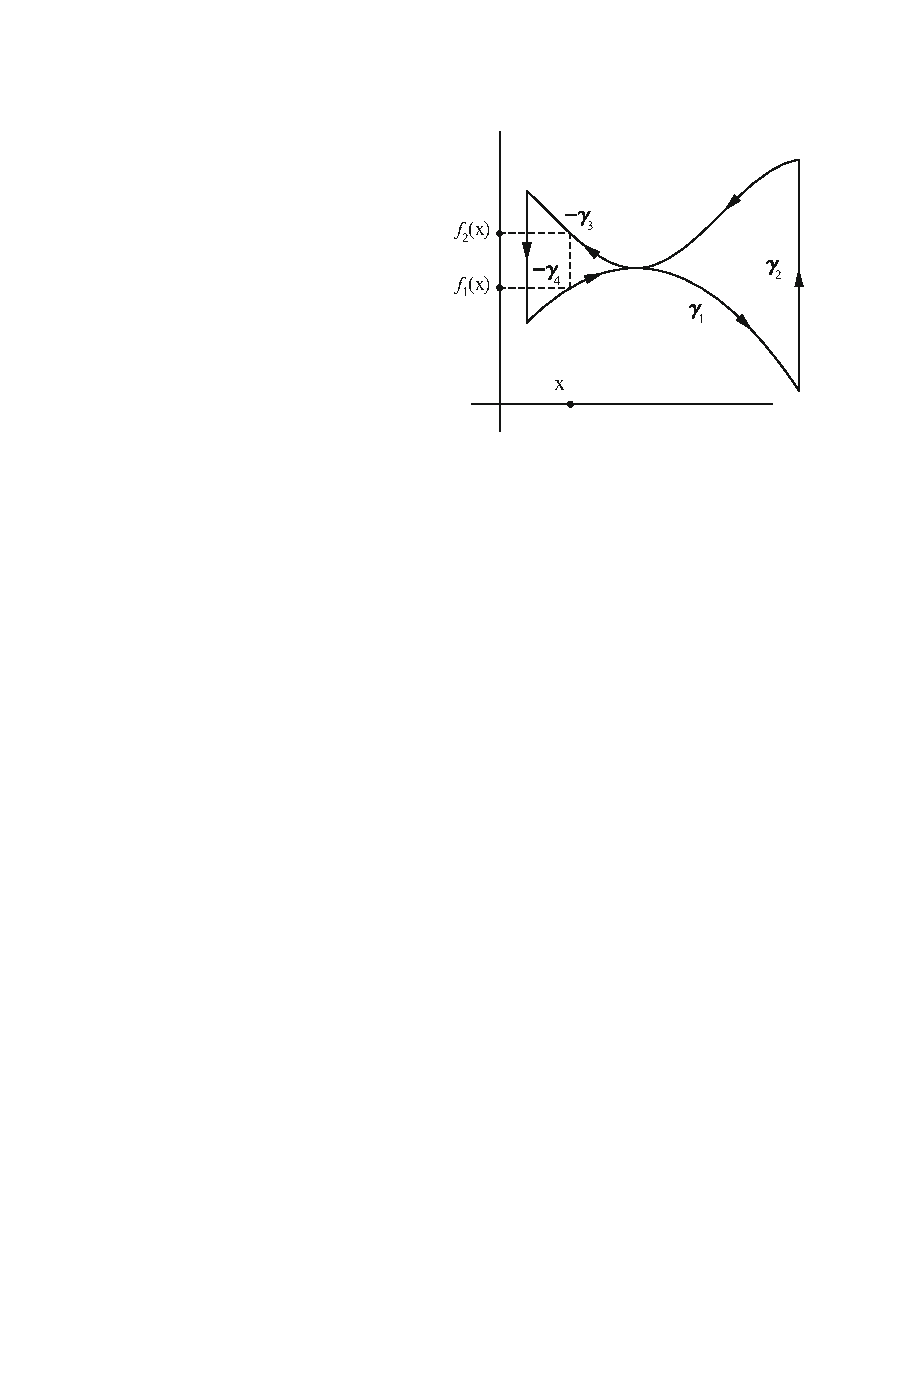
\includegraphics[width=0.5\linewidth]{regoin of type I.pdf}
    \caption{}
    \label{fig:enter-label}
\end{figure}

\begin{definition}
يُقال إن المجموعة المدمجة \( K \subset \mathبب{R}^2 \) هي منطقة من النوع الأول (الشكل 2.7) إذا كان من الممكن وصفها كالتالي:
\[ K = \{ (x, y) \in \mathبب{R}^2 : a \leq x \leq b، f_1(x) \leq y \leq f_2(x) \}، \]
حيث \( f_1، f_2 : [a، b] \to \mathبب{R} \) هما دالتان مستمرتان من الفئة \( C^1 \) جزئيًا، و \( f_1 \leq f_2 \).
\end{definition}

الحدود الموجهة إيجابيًا لـ \( K \) هي اتحاد المسارات \( \gamma = \gamma_1 \cup \gamma_2 \cup (-\gamma_3) \cup (-\gamma_4) \)، حيث:
\[ \gamma_1 : [a، b] \to \mathبب{R}^2، \gamma_1(t) := (t، f_1(t))؛ \]
\[ \gamma_2 : [f_1(b)، f_2(b)] \to \mathبب{R}^2، \gamma_2(t) := (b، t)؛ \]
\[ \gamma_3 : [a، b] \to \mathبب{R}^2، \gamma_3(t) := (t، f_2(t))؛ \]
\[ \gamma_4 : [f_1(a)، f_2(a)] \to \mathبب{R}^2، \gamma_4(t) := (a، t). \]

\begin{lemma}
لنفترض أن \( K \) هي مجموعة مدمجة ومنطقة من النوع الأول وأن \( P \) هي دالة مستمرة على \( K \) وتقبل مشتق جزئي مستمر \( \frac{\partial P}{\partial y} \) في جوار \( K \). إذن
\[ \oint_{\partial K} P \، dx = - \iint_K \frac{\partial P}{\partial y} \، d(x، y). \]
\end{lemma}

\begin{demonstration}
بما أن \( \gamma_1'(t) = (1، f_1'(t))، \gamma_2'(t) = (0، 1)، \gamma_3'(t) = (1، f_2'(t))، \gamma_4'(t) = (0، 1) \) لكل \( t \)، لدينا
\[ \oint_{\gamma} P \، dx = \int_{a}^{b} P(t، f_1(t)) \، dt - \int_{a}^{b} P(t، f_2(t)) \، dt. \]

من ناحية أخرى، كل دالة مستمرة على مجموعة مدمجة \( K \) تكون قابلة للتكامل، ووفقًا لنظرية فوبيني،
\[ \iint_K \frac{\partial P}{\partial y} \، d(x، y) = \int_{a}^{b} \left( P(x، f_2(x)) - P(x، f_1(x)) \right) \، dx. \]

بمقارنة هاتين المعادلتين، لدينا
\[ \oint_{\partial K} P \، dx = - \iint_K \frac{\partial P}{\partial y} \، d(x، y). \]
\end{demonstration}

نص نظرية غرين على أن التكامل الخطي لحقل متجه على محيط منحنى مغلق يعادل تكامل التدفق عبر المساحة المحصورة داخل المنحنى. بشكل رياضي, إذا كان \(C\) منحنى مغلق في المستوى, و \(D\) هي المساحة المحصورة داخل \(C\), فإن:
\[ \oint_C (L \, dx + M \, dy) = \iint_D \left( \frac{\partial M}{\partial x} - \frac{\partial L}{\partial y} \right) dx \, dy. \]

\begin{lemma}
إذا كان \(F : U \subset \mathbb{R}^2 \to \mathbb{R}^2\) حقل متجه من الدرجة \(C^1\) وكان \(C\) منحنى مغلق بسيط بحيث أن \(C = \partial D\) لبعض المنطقة \(D\) في \(U\), فإن:
\[ \oint_C F \cdot dr = \iint_D \left( \frac{\partial N}{\partial x} - \frac{\partial M}{\partial y} \right) dx \, dy, \]
حيث أن \(F = (M, N)\).
\end{lemma}

\begin{demonstration}
نظرية غرين تعطينا مباشرة أن التكامل الخطي للحقل المتجه \(F\) حول المنحنى المغلق \(C\) يساوي التكامل الثنائي لتباعد الحقل المتجه عبر المساحة \(D\) المحصورة داخل \(C\).
\end{demonstration}


على الرغم من الاختلافات بين نظريتي التكامل, وتفضيلنا لنظرية ليبيغ, يجب على القارئ أن يكون على دراية بأنه لأغراضنا, ومع الجهد الكافي, من الممكن أن نُظهر أن معظم الحالات التي نواجهها في النص تناسب إطار تكامل ريمان ومحتوى جوردان, وبالتالي يمكن للقارئ أن يستمر في التفكير والتصور من حيث تكامل ريمان. لكننا لن نسد هذه الفجوة صراحة هنا. كتاب يتناول كلا النظريتين ويمكن مقارنتهما هو كتاب أبوستول.

\begin{definition}
\begin{itemize}
    \item [(i)] تُسمى مجموعة \( R = \Pi_{j=1}^n I_j \) مستطيل \( n \) في \( \mathbb{R}^n \) إذا كان كل \( I_j \) فترة محدودة في \( \mathbb{R} \), أي إذا وجدت الأعداد الحقيقية \( a_j \leq b_j \) بحيث \( (a_j, b_j) \subseteq I_j \subseteq [a_j, b_j] \) لكل \( j = 1, \ldots, n \). في هذه الحالة, يتم تعريف مقياس ليبيغ لـ \( R \) كـ
    \[ m(R) = \Pi_{j=1}^n (b_j - a_j). \]
    \item[(ii)] تُسمى المجموعة الفرعية \( N \) من \( \mathbb{R}^n \) مجموعة عديمة إذا كان لأي \( \epsilon > 0 \), توجد سلسلة من المستطيلات \( n \) $(R_k)$ بحيث \( N \subseteq \cup_{k=1}^{\infty} R_k \) و
    \[ \sum_{k=1}^{\infty} m(R_k) < \epsilon. \]
    \item[(iii)] يُقال أن خاصية \( P(x) \) حيث \( x \in \mathbb{R}^n \) صحيحة تقريبًا في كل مكان إذا وجدت مجموعة عديمة \( N \subset \mathbb{R}^n \) بحيث تكون الخاصية \( P(x) \) صحيحة لكل \( x \in \mathbb{R}^n \setminus N \).
    \item[(iv)] بالنظر إلى مجموعة فرعية \( K \) من \( \mathbb{R}^n \), يتم تعريف الدالة المميزة لـ \( K \), والتي تُرمز بـ \( \chi_K \), كما يلي:
    \[ \chi_K(x) = \begin{cases} 
    1 & \text{إذا } x \in K \\
    0 & \text{إذا } x \notin K 
    \end{cases} \]
    \item[(v)] تُسمى الدالة \( \varphi : \mathbb{R}^n \to \mathbb{R} \) دالة خطوات إذا كانت مزيجًا خطيًا من الدوال المميزة للمستطيلات \( n \), أي إذا
    \[ \varphi = \sum_{k=1}^m c_k \chi_{R_k}, \]
حيث \( c_k \in \mathbb{R} \) و \( R_k \) هو مستطيل \( n \).
    \item[(vi)] تُقال المجموعة الفرعية \( M \subset \mathbb{R}^n \) قابلة للقياس إذا وجدت سلسلة $(\varphi_h)\infty_h=1$ من دوال الخطوات ومجموعة عديمة $N$ من \( \mathbb{R}^n \) بحيث تتقارب سلسلة الأعداد الحقيقية $(\varphi_h(x))$ إلى \( \chi_M(x) \) لكل \( x \in \mathbb{R}^n \setminus N \), أي إذا كانت السلسلة $(\varphi_h)\infty_h=1$ 
تتقارب تقريبًا في كل مكان إلى \( \chi_M \).
\end{itemize}
\end{definition}

يمكن إثبات أنه لأي \(\epsilon > 0\), يمكن تغطية مجموعة عديمة بسلسلة من المكعبات \( (R_k) \) التي هي مستطيلات \( n \) بأطوال جوانب متساوية, بحيث
\[ \sum_{k=1}^{\infty} m(R_k) < \epsilon. \]

ستكون عائلة المجموعات القابلة للقياس ليبيغ في \( \mathbb{R}^n \) مهمة جدًا طوال الوقت, لكننا نحتاج فقط إلى الحقائق الأساسية التالية حول هذه العائلة:

1. كل مجموعة مفتوحة وكل مجموعة مغلقة في \( \mathbb{R}^n \) قابلة للقياس.
2. إذا كانت \( M \) مجموعة قابلة للقياس, فإن \( \mathbb{R}^n \setminus M \) أيضًا قابلة للقياس.
3. إذا كانت \( (M_k) \) عائلة (قابلة للعد) من المجموعات القابلة للقياس, فإن \( \cap_{k=1}^{\infty} M_k \) و \( \cup_{k=1}^{\infty} M_k \) مجموعات قابلة للقياس أيضًا.
4. كل مجموعة عديمة قابلة للقياس ليبيغ.

سنحتاج إلى استخدام نظرية فوبيني, ولذلك سنذكرها. نتبع ترميز سترومبرج [18, نظرية 6.121, ص. 352] ونشير إلى ذلك الكتاب لتعريف تكامل ليبيغ في \( \mathbb{R}^n \). يُرمز إلى فضاء الدوال القابلة للتكامل ليبيغ في \( \mathbb{R}^n \) بـ \( L(\mathbb{R}^n) \). إذا كانت \( A \) مجموعة قابلة للقياس في \( \mathbb{R}^n \), سنقول إن الدالة \( f : A \to \mathbb{R} \) قابلة للتكامل ليبيغ على \( A \) إذا تم تمديدها كصفر خارج \( A \) وتم ترميز هذا التمديد بـ \( f \chi_A \), فإن الدالة \( f \chi_A \) قابلة للتكامل ليبيغ على \( \mathbb{R}^n \). في هذه الحالة, وفقًا للتعريف,
\[ \int_A f := \int_A f(x) \, dx := \int_{\mathbb{R}^n} f \chi_A(x) \, dx. \]

إذا كانت \( A = [a, b] \), نحافظ على الترميز الكلاسيكي ونكتب
\[ \int_{[a,b]} f(x) \, dx = \int_a^b f(x) \, dx. \]

في حالة أن \( f \) تحتوي على متغيرين أو ثلاثة, سنكتب
\[ \int_A f(x, y) \, d(x, y) \text{ أو } \int_A f(x, y, z) \, d(x, y, z). \]

نفضل كتابة \( d(x, y) \) بدلاً من \( dx \, dy \) لتجنب الخلط مع حاصل الضرب الخارجي \( dx \wedge dy \) (انظر الفصل السادس).



**النظرية 2.6.1 (نظرية فوبيني).**
لنفترض أن \( f \in L(\mathbb{R}^{n+p}) \). إذن:

(i) \( f_x(y) = f(x, y) \) ينتمي إلى \( L(\mathbb{R}^p) \) تقريبًا في كل مكان في \( \mathbb{R}^n \).

(ii) \( f_y(x) = f(x, y) \) ينتمي إلى \( L(\mathbb{R}^n) \) تقريبًا في كل مكان في \( \mathbb{R}^p \).

(iii) \( F(x) := \int_{\mathbb{R}^p} f_x(y) \, dy \) معرّف (أي أن التكامل موجود) تقريبًا في كل مكان في \( \mathbb{R}^n \) وهو قابل للتكامل ليبيغ في \( \mathbb{R}^n \). كذلك \( G(y) := \int_{\mathbb{R}^n} f_y(x) \, dx \) معرّف تقريبًا في كل مكان في \( \mathbb{R}^p \), وعلاوة على ذلك, \( G \) ينتمي إلى \( L(\mathbb{R}^p) \).

\[ \int_{\mathbb{R}^n} \left( \int_{\mathbb{R}^p} f(x, y) \, dy \right) \, dx = \int_{\mathbb{R}^{n+p}} f(x, y) \, d(x, y) = \int_{\mathbb{R}^p} \left( \int_{\mathbb{R}^n} f(x, y) \, dx \right) \, dy. \]

متغير لنظرية فوبيني يكون مفيدًا لنا هو التالي. لنفترض أن \( A \subset [a, b] \times [c, d] \) مجموعة قابلة للقياس وأن \( f : A \to \mathbb{R} \) دالة قابلة للتكامل ليبيغ على \( A \). لكل \( x \in [a, b] \), لنعرّف \( A_x = \{ y \in \mathbb{R} : (x, y) \in A \} \). إذن:

\[ \int_A f(x, y) \, d(x, y) = \int_a^b \left( \int_{A_x} f(x, y) \, dy \right) \, dx. \]

المفهوم التالي سيتم مناقشته بشكل أكثر دقة في القسم 8.5.

**التعريف 2.6.2.** لنفترض أن \( K \subset \mathbb{R}^2 \) مجموعة مدمجة بحيث أن حدودها \( \partial K \) تساوي \( \gamma([a, b]) \), حيث \( \gamma : [a, b] \to \mathbb{R}^2 \) مسار مغلق جزئيًا من الفئة \( C^1 \). نقول إن \( \gamma \) موجهة إيجابيًا إذا مرت \( \gamma \) على \( \partial K \) مرة واحدة بحيث أن المنطقة \( K \) دائمًا تقع إلى اليسار (انظر الشكل 2.8). لكي نكون دقيقين, يجب أن نفترض أن المجموعة المدمجة \( K \) تحقق الشرط (8.10), انظر على سبيل المثال كارتان [7, 4.4.1].

**النظرية 2.6.2 (نظرية غرين).** لنفترض أن \( K \subset \mathbb{R}^2 \) مجموعة مدمجة ذات حدود موجهة إيجابيًا يحددها \( \gamma \) (كما في التعريف 2.6.2). لنفترض أن \( \omega = P \, dx + Q \, dy \) شكل تفاضلي من الدرجة 1 من الفئة \( C^1 \) في مجموعة مفتوحة \( U \subset \mathbb{R}^2 \) بحيث \( K \subset U \). إذن:

\[ \oint_{\gamma} (P \, dx + Q \, dy) = \iint_K \left( \frac{\partial Q}{\partial x} - \frac{\partial P}{\partial y} \right) \, d(x, y). \]

باستخدام ترميز الحقول المتجهة, يمكن كتابة ذلك كالتالي:

\[ \oint_{\gamma} (\mathbf{P}, \mathbf{Q}) = \iint_K \left( \frac{\partial Q}{\partial x} - \frac{\partial P}{\partial y} \right) \, d(x, y). \]

\begin{figure}
    \centering
    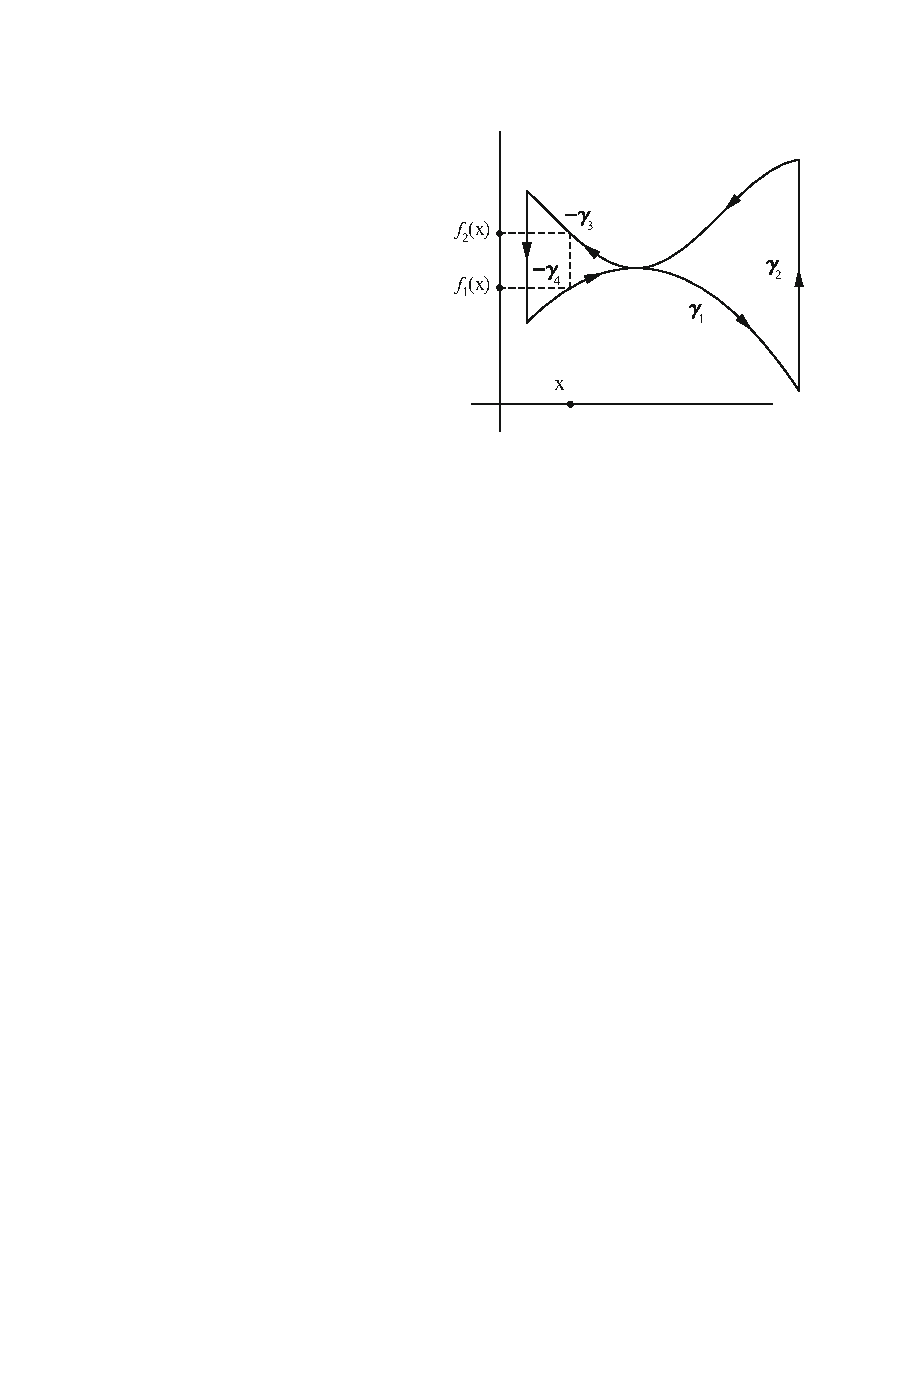
\includegraphics[width=0.5\linewidth]{regoin of type I.pdf}
    \caption{}
    \label{fig:enter-label}
\end{figure}

قد يشعر القارئ بعدم الارتياح مع التعريف 2.6.2 والنظرية 2.6.2. هذا متوقع ومرحب به. لقد واجهنا للمرة الأولى تباينًا معينًا يتم التغاضي عنه غالبًا أو تجنبه, ولكن يجب علينا معالجته بشكل محدد في هذا الكتاب. يتمتع التعريف 2.6.2 والنظرية 2.6.2 بصياغة بديهية ورياضية دقيقة, وهذه الصياغات ليست سهلة التوفيق. إذا نظرنا إلى نظرية غرين من منظور بديهي (عادةً ما يكون ذلك في سياق حساب التفاضل والتكامل المتجه), فإن الصعوبة الحقيقية لا توجد عمومًا. على سبيل المثال, إذا أردنا تطبيقها على الحالات الناشئة في المشكلات الفيزيائية, فإن ما يعنيه اليسار واليمين يكون واضحًا, ولا نتوقع أي صعوبة في تحديد ما إذا كانت المنطقة \( K \) تقع إلى اليسار. ومع ذلك, من وجهة نظر رياضية بحتة (أي, في سياق التحليل المتجهي), فإن تفسير "اليسار" و"اليمين" ليس واضحًا على الإطلاق, وسيتطلب منا جهدًا كبيرًا لتطوير الأدوات المناسبة للتعامل مع هذا المفهوم. لاحقًا, في الفصول 5 و9, سنقدم تعريفًا دقيقًا للتوجيه ونسخة عامة من نظرية غرين. في الوقت الحالي, سنكتفي بالعمل نحو إثبات النظرية في بعض المناطق المحددة \( K \) التي يمكن تعريف التوجيه فيها بسهولة, والتي يتطابق تعريف التوجيه فيها مع حدسنا الفيزيائي.

**التعريف 2.6.3.** يُقال إن المجموعة المدمجة \( K \subset \mathbb{R}^2 \) منطقة من النوع الأول (الشكل 2.9) إذا كان يمكن وصفها على النحو التالي:
\[ K = \{ (x, y) \in \mathbb{R}^2 : a \leq x \leq b, f_1(x) \leq y \leq f_2(x) \}, \]
حيث \( f_1 \) و \( f_2 \) دوال جزئية من الفئة \( C^1 \), و \( f_1 \leq f_2 \).

الحدود الموجهة إيجابيًا لـ \( K \) هي اتحاد المسارات \( \gamma = \gamma_1 \cup \gamma_2 \cup (-\gamma_3) \cup (-\gamma_4) \), حيث:
\[ \gamma_1 : [a, b] \to \mathbb{R}^2, \gamma_1(t) := (t, f_1(t))؛ \]
\[ \gamma_2 : [f_1(b), f_2(b)] \to \mathbb{R}^2, \gamma_2(t) := (b, t)؛ \]
\[ \gamma_3 : [a, b] \to \mathbb{R}^2, \gamma_3(t) := (t, f_2(t))؛ \]
\[ \gamma_4 : [f_1(a), f_2(a)] \to \mathbb{R}^2, \gamma_4(t) := (a, t). \]

**اللمّة 2.6.1.** لنفترض أن \( K \) مجموعة مدمجة من النوع الأول وأن \( P \) دالة مستمرة على \( K \) تقبل مشتقة جزئية مستمرة \( \frac{\partial P}{\partial y} \) في جوار \( K \). إذن:

\[ \oint_{\gamma} P \, dx = -\iint_K \frac{\partial P}{\partial y} \, d(x, y). \]

الدليل: بما أن \( \gamma_1'(t) = \gamma_1'(t) = (0, 1) \), \( \gamma_3'(t) = (1, f_3'(t)) \), و \( \gamma_3'(t) = (1, f_3'(t)) \) لكل \( t \), لدينا:

\[ 
\oint_{\gamma} P \, dx = \int_a^b P(t, f_1(t)) \, dt - \int_a^b P(t, f_2(t)) \, dt.
\]

من ناحية أخرى, كل دالة مستمرة على مجموعة مدمجة \( K \) هي قابلة للتكامل, ووفقًا لنظرية فوبيني:
\[ \iint_K \frac{\partial P}{\partial y} \, d(x, y) = \int_a^b \left( \int_{f_1(x)}^{f_2(x)} \frac{\partial P}{\partial y} (x, y) \, dy \right) dx = \int_a^b (P(x, f_2(x)) - P(x, f_1(x))) \, dx. \]

بمقارنة هاتين المعادلتين, نحصل على:

\[ \oint_{\gamma} P \, dx = -\iint_K \frac{\partial P}{\partial y} \, d(x, y). \]

**التعريف 2.6.4.** يُقال إن المجموعة المدمجة \( K \subset \mathbb{R}^2 \) منطقة من النوع الثاني (الشكل 2.10) إذا كان يمكن وصفها على النحو التالي:
\[ K = \{ (x, y) : c \leq y \leq d؛ g_1(y) \leq x \leq g_2(y) \}, \]
حيث \( g_1 \) و \( g_2 \) دوال جزئية من الفئة \( C^1 \), و \( g_1 \leq g_2 \).

الحدود الموجهة إيجابيًا لـ \( K \) هي اتحاد المسارات \( \gamma = (-\gamma_1) \cup \gamma_2 \cup \gamma_3 \cup (-\gamma_4) \), حيث:
\[ \gamma_1 : [c, d] \to \mathbb{R}^2, \gamma_1(t) := (g_1(t), t)؛ \]
\[ \gamma_2 : [g_1(c), g_2(c)] \to \mathbb{R}^2, \gamma_2(t) := (t, c)؛ \]
\[ \gamma_3 : [c, d] \to \mathbb{R}^2, \gamma_3(t) := (g_2(t), t)؛ \]
\[ \gamma_4 : [g_1(d), g_2(d)] \to \mathbb{R}^2, \gamma_4(t) := (t, d). \]


**اللمّة 2.6.2.** لنفترض أن \( K \) مجموعة مدمجة وهي منطقة من النوع الثاني, ولنفرض أن \( Q \) دالة مستمرة على \( K \) وتقبل مشتقة جزئية مستمرة \( \frac{\partial Q}{\partial x} \) في جوار \( K \). إذن:

\[ \oint_{\gamma} Q \, dy = \iint_K \frac{\partial Q}{\partial x} \, d(x, y). \]

**النظرية 2.6.3.** لنفترض أن \( K \) منطقة من النوع الأول أو منطقة من النوع الثاني, ولنفترض أن \( \omega = P \, dx + Q \, dy \) شكل تفاضلي من الدرجة 1 من الفئة \( C^1 \) على بعض المستطيلات المفتوحة التي تحتوي على \( K \). إذن:

\[ \oint_{\gamma} P \, dx + Q \, dy = \iint_K \left( \frac{\partial Q}{\partial x} - \frac{\partial P}{\partial y} \right) \, d(x, y). \]

الدليل: نختار \( a \), \( b \), \( c \), و \( d \) بحيث تكون \( K \) محتواة في المستطيل \( R = [a, b] \times [c, d] \) ونفترض أن الشكل التفاضلي \( \omega \) معرف وهو من الفئة \( C^1 \) على المستطيل المفتوح \( T \) الذي يحتوي على \( R \). سنعرض الدليل في حالة أن \( K \) منطقة من النوع الأول. في حالة أن \( K \) منطقة من النوع الثاني, فإن حجة مشابهة تؤدي إلى نفس النتيجة.

لقد أثبتنا بالفعل أن:

\[ \oint_{\gamma} P \, dx = -\iint_K \frac{\partial P}{\partial y} \, d(x, y), \]

ولذلك نحتاج فقط إلى الحصول على:

\[ \oint_{\gamma} Q \, dy = \iint_K \frac{\partial Q}{\partial x} \, d(x, y). \]

لاحظ أننا لا يمكننا تطبيق اللمّة السابقة, لأن \( K \) ليست بالضرورة منطقة من النوع الثاني. نتابع كما يلي.

لكل \( (x, y) \in T \), نعرّف \( V(x, y) := \int_c^y Q(x, t) \, dt \). الدالة الناتجة \( V \) لها خاصية أن:

\[ dV(x, y) = F(x, y) \, dx + Q(x, y) \, dy, \]

حيث:

\[ F(x, y) = \int_c^y \frac{\partial Q}{\partial x} (x, t) \, dt. \]

تم الحصول على التعبير عن \( F \) بعد تطبيق الاقتراح 2.5.1 (انظر أيضًا أبوستول [1, نظرية 10.39]). وفقًا للنظرية 2.5.1, لدينا:

\[ dV = 0, \]

لذلك:

\[ \oint_{\gamma} Q(x, y) \, dy = -\oint_{\gamma} F(x, y) \, dx. \]

علاوة على ذلك, \( K \) هي منطقة من النوع الأول, وفي جوار \( K \):

\[ \frac{\partial F}{\partial y} (x, y) = \frac{\partial Q}{\partial x} (x, y). \]

تطبيق اللمّة 2.6.1 على \( F(x, y) \, dx \) يعطينا:

لأن لكل \( x \) ثابت, تكون الدالة \( y \to F(x, y) \) بدائية لـ \( y \to \frac{\partial Q}{\partial x} (x, y). \)

أخيرًا:

\[ \oint_{\gamma} Q \, dy = \iint_K \frac{\partial Q}{\partial x} \, d(x, y), \]

و:

\[ \oint_{\gamma} P \, dx + Q \, dy = \iint_K \left( \frac{\partial Q}{\partial x} - \frac{\partial P}{\partial y} \right) \, d(x, y). \]


**التعريف 2.6.5.** تُقال أن المجموعة المدمجة \( K \) هي منطقة بسيطة إذا كانت \( K \) منطقة من النوع الأول وأيضًا منطقة من النوع الثاني.

يمكن تخفيف الفرضية الخاصة بنظرية غرين على المناطق البسيطة إلى حد ما, حيث يكفي أن يكون الشكل التفاضلي من الدرجة الأولى معرفًا في جوار \( K \). قبل تقديم الدليل, دعونا نحدد اتفاقية الترميز التي تكون صالحة بناءً على الحقيقة التالية (انظر الاقتراح 2.7.2). لنفترض أن \( K \) منطقة بسيطة و \( \gamma_1 : [a, b] \to \mathbb{R}^2 \), \( \gamma_2 : [c, d] \to \mathbb{R}^2 \) هما مساران بسيطان, مغلقان, وقطعيا ناعمان مع
\[ \gamma_1([a, b]) = \gamma_2([c, d]) = \partial K \]
وبحيث أن \( \gamma_1 \) و \( \gamma_2 \) ينتجان نفس التوجيه على الحدود \( \partial K \). إذن وفقًا للاقتراح 2.7.2,
\[ \oint_{\gamma_1} \omega = \oint_{\gamma_2} \omega. \]

بالتالي, من المنطقي كتابة
\[ \oint_{\partial K} \omega \]
إذا فسرنا التكامل على أنه تم على طول أي مسار بسيط, مغلق, وقطعيًا \( C^1 \) يعطي تبارجعًا لـ \( \partial K \) بحيث تكون المنطقة \( K \) دائمًا على اليسار.

**النظرية 2.6.4.** لنفترض أن \( K \subset \mathbb{R}^2 \) منطقة بسيطة وأن \( \omega = P \, dx + Q \, dy \) شكل تفاضلي من الدرجة الأولى من الفئة \( C^1 \) على جوار مفتوح لـ \( K \). إذن:

\[
\oint_{\partial K} \omega = \iint_K \left( \frac{\partial Q}{\partial x} - \frac{\partial P}{\partial y} \right) \, d(x, y).
\]

الدليل: بما أن \( K \) منطقة من النوع الأول, لدينا:

\[ 
\oint_{\partial K} P \, dx = -\iint_K \frac{\partial P}{\partial y} \, d(x, y), 
\]

وبما أنها أيضًا منطقة من النوع الثاني, نحصل على:
\[ 
\oint_{\partial K} Q \, dy = \iint_K \frac{\partial Q}{\partial x} \, d(x, y). 
\]

يكفي جمع هاتين الهويتين.

تسمح لنا صيغة غرين بتقديم دليل مباشر لشرط الكفاية لحقل المتجه ليكون محافظًا (النظرية 2.5.6) على مجموعة مفتوحة ونجومية في المستوى.


**النظرية 2.6.5 (لمّة بوانكاريه).** لنفترض أن \( F = (P, Q) \) حقل متجه من الفئة \( C^1 \) على المجموعة المفتوحة والنجومية \( U \subset \mathbb{R}^2 \) ونفترض أن:

\[ \frac{\partial Q}{\partial x} = \frac{\partial P}{\partial y} \]
لكل \( (x, y) \in U \). إذن \( F \) هو حقل متجه محافظ.

الدليل: لنفترض أن \( \omega = P \, dx + Q \, dy \) هو الشكل التفاضلي المرتبط بحقل المتجه \( F \). يكفي إثبات أن:


\[ \oint_{\partial K} \omega = 0 \]
كلما كانت \( \partial K \) حدود مثلث ما \( K \) محتواة في \( U \). بما أن \( K \) منطقة بسيطة, فإنه يتبع من نظرية غرين أن:

\[ \oint_{\partial K} (P \, dx + Q \, dy) = \iint_K \left( \frac{\partial Q}{\partial x} - \frac{\partial P}{\partial y} \right) \, d(x, y) = 0. \]

ستُعرض نسخة عامة من لمّة بوانكاريه على \( \mathbb{R}^n \) في الفصل السادس (انظر القسم 6.6) بعد أن نكمل دراستنا للأشكال التفاضلية.
\newpage

\section{التمارين}
\subsection{}
احسب طول المسار
\[ \gamma(t) = (e^t \cos(t), e^t \sin(t)), \]
للفترة \( 0 \leq t \leq \pi \).
\subsection{}
احصل على تبارجع, عكس اتجاه عقارب الساعة, للإهليلج
\[ \frac{x^2}{a^2} + \frac{y^2}{b^2} = 1 \] 
(حيث \( a, b > 0 \)).

\subsection{}
تكامل حقل المتجه
\[ F(x, y) = (y^2, -2xy) \]
على طول المثلث ذو الرؤوس \((0, 0), (1, 0), (0, 1)\), مع الاتجاه عكس اتجاه عقارب الساعة.

\subsection{}
(1) جد مسارًا \( \gamma \) يكون مساره هو تقاطع الأسطوانة \( x^2 + y^2 = 1 \) مع المستوي \( x + y + z = 1 \) ومع الخصائص الإضافية أن النقطة الابتدائية (والنقطة النهائية) هي \((0, -1, 2)\) والإسقاط على مستوى \( xy \) هو باتجاه عكس عقارب الساعة.
(2) احسب:
\[ \int_{\gamma} (x \, dy + y \, dz - x \, dz). \]

\subsection{}
لنفترض أن \( \gamma \) هو مسار بسيط يكون مساره هو تقاطع المستويات الإحداثية مع جزء الكرة الوحدة في الربع الأول, موجهًا وفقًا للتسلسل \((1, 0, 0), (0, 1, 0), (0, 0, 1), (1, 0, 0)\). احسب:
\[ \int_{\gamma} (z \, dx + x \, dy + y \, dz). \]
\subsection{}
جد مسارًا يكون مساره هو تقاطع نصف الكرة العلوي ذي نصف القطر \( 2a \) مع الأسطوانة
\[ x^2 + y^2 + z^2 = 4a^2, x^2 + (y - a)^2 = a^2. \]

\subsection{}
حدد ما إذا كان حقل المتجه
\[ F : \mathbb{R}^2 \to \mathbb{R}^2, F(x, y) = (x^3y, x) \]
محافظًا.
\subsection{}
جد دالة جهد لحقل المتجه
\[ F : \mathbb{R}^2 \to \mathbb{R}^2, F(x, y) = (2xy, x^2 - y^2). \]
\subsection{}
لحقل المتجه
\[ F : \mathbb{R}^3 \to \mathbb{R}^3, F(x, y, z) = (2xy, x^2 + z^2, 2zy), \]
(1) أثبت أن \( \nabla \times F = 0 \);
(2) جد دالة جهد لـ \( F \).
\subsection{}
(1) أثبت أن حقل المتجه
\[
F(x, y) = \left(e^x(\sin(x + y) + \cos(x + y)) + 1, e^x \cos(x + y) \right)
\]
محافظ على \( \mathbb{R}^2 \) واجد دالة جهد.
\\
(2) احسب التكامل الخطي
\[ \int_{\gamma} F, \]
حيث
\[ \gamma : [0, \pi] \to \mathbb{R}^2;\, \gamma(t) = (\sin(\pi e^{\sin(t)})), \cos^5(t)). \]
\subsection{}
احسب
\[ 
\int_{\gamma} x \, dx + y \, dy + z \, dz, 
\]
حيث:
\[ \gamma(t) = (\cos^4(t), \sin^2(t) + \cos^3(t), t), 0 \leq t \leq \pi. \]

\subsection{}
للحقل المتجه
\[ F = (f_1, f_2) : \mathbb{R}^2 \setminus \{(0, 0)\} \to \mathbb{R}^2, \]
المعرف بـ:
\[ f_1(x, y) = -\frac{y}{x^2 + y^2}, f_2(x, y) = \frac{x}{x^2 + y^2}, \]

(1) أثبت أن
\[ \frac{\partial f_2}{\partial x}(x, y) = \frac{\partial f_1}{\partial y}(x, y) \]
لكل \( (x, y) \in \mathbb{R}^2 \setminus \{(0, 0)\).

(2) لنفترض أن \( \gamma \) هي الدائرة الوحدة موجهة بعكس اتجاه عقارب الساعة. أثبت أن
\[ \oint_{\gamma} F = 2\pi. \]
هل هذه الحقيقة تتناقض مع لمّة بوانكاريه؟

(3) ناقش ما إذا كان هذا البيان صحيحًا: لكل مسار مغلق وقطعيًا من الفئة \( C^1 \) \( \alpha : [a, b] \to \mathbb{R}^2 \setminus \{(0, 0)\} \) بحيث \( \alpha_1(t) \geq 0 \) لكل \( t \in [a, b] \),
\[ \oint_{\alpha} F = 0. \]

(4) احسب \( \oint_{\gamma} F \), حيث
\[ \gamma(t) = (\cos(t), \sin^7(t)), -\frac{\pi}{2} \leq t \leq \frac{\pi}{2}. \]
\subsection{}
لنفرض أن \( \gamma(t) = (\cos(t), \sin(t)) \) معطاة ولننظر في المسارين
\[ \alpha := \gamma|_{[-\pi, \pi]} \text{ و } \beta := \gamma|_{[0, 2\pi]}. \]

(1) هل \( \alpha \) و \( \beta \) مساران مكافئان؟

(2) برر لماذا
\[ \oint_{\alpha} F = \oint_{\beta} F \]
لكل حقل متجه مستمر \( F : U \subset \mathbb{R}^2 \to \mathbb{R}^2 \) معرف على الدائرة الوحدة.
\subsection{}
لنفترض أن \( \gamma \) هو المسار الذي يكون مساره اتحاد رسم الدالة \( y = x^3 \) من النقطة (0, 0) إلى النقطة (1, 1) والقطعة من النقطة (1, 1) إلى النقطة (0, 0). باستخدام نظرية غرين, احسب:
\[ \int_{\gamma} (x^2 + y^2) \, dx + (2xy + x^2) \, dy. \]
\subsection{}
استخدم نظرية غرين لحساب التكامل الخطي:
\[ 
\int_{\gamma} (x^2 + 3x^2y^2) \, dx + (2x^3y + x^2) \, dy, 
\]
حيث \( \gamma \) هو الحد الفاصل للمنطقة الواقعة بين رسوم \( y = 0 \) و \( y = 4 - x^2 \), موجهة بعكس اتجاه عقارب الساعة.
\subsection{}
لنفترض أن \( K \) منطقة من النوع الأول أو النوع الثاني وأن \( \gamma \) مسار يكون مساره هو الحد الفاصل لـ \( K \) موجهًا بعكس اتجاه عقارب الساعة. إذن:
\[ \text{area}(K) = \frac{1}{2} \oint_{\gamma} (-y \, dx + x \, dy) = \frac{1}{2} \oint_{\gamma} -y \, dx = \frac{1}{2} \oint_{\gamma} x \, dy. \]
\subsection{}
احسب المساحة المحاطة بالدوارة \( \gamma : [0, 2\pi] \to \mathbb{R}^2 \),
\[ \gamma(t) = (at - a\sin(t), a - a\cos(t)) \]
(حيث \( a > 0 \)) ومحور \( x \).
\subsection{}
احسب المساحة المحاطة بالمحورين الإحداثيين والمسار
\[ \gamma(t) = (\sin^4(t), \cos^4(t)), 0 \leq t \leq \pi. \]
\subsection{}
احسب المساحة المحصورة بين الدائرتين
\[ C_1: (x, y) \in \mathbb{R}^2 : x^2 + y^2 = a^2 \]
و
\[ C_2: (x, y) \in \mathbb{R}^2 : x^2 + y^2 = 2ax  ( a > 0 ). \]


\chapter{إضافة الملحقات}

\section{استدعاء class}

\LR{\begin{lstlisting} 
\documentclass[<options>]{mathbook_arabic}
\end{lstlisting}}




\subsection{الخيارات}\index{خيارات}
 \begin{itemize}
 \item
 حجم الخط
  10pt, 11pt, 12pt,
 \end{itemize}

\LR{\begin{lstlisting} 
%Example
\documentclass[a4paper,12pt]{mathbook_arabic}
\end{lstlisting}}
 
 
\chapter{الألوان والخطوط والأطوال}
 

  \section{الألوان المستخدمة}\index{ألوان}

 تم تعريف الألون  في الملف
\ee{colors\textunderscore2.tex}
 باستخدام تعليمة
 
\LR{\begin{lstlisting} 
\definecolor{<name color>}{cmyk}{<num>,<num>,<num>}
%Example
\definecolor{chapter@bg@color}{cmyk}{1,0.2,0.3,0.1}
\end{lstlisting}}
 
 
\subsection{تغيير الألوان}\index{تعريف الألوان}
\LR{\begin{lstlisting}
\redefineColor{<nom de la couleur>}{<nouvelle valeur CMYK}
% Exemple :
\makeatletter
\redefineColor{arrayrule@color}{0,0,0,1} % for "black"
\makeatother
\end{lstlisting}}




\section{الخطوط}\index{خطوط}




\subsection{الخطوط المتسخدمة}
تم استخدام الخط Amiri
للغة العربية بشكل افتراضي 
بإضافة :
\LR{\begin{lstlisting}
\newfontfamily\arabicfont[Script=Arabic]{Amiri}
\end{lstlisting}}




\vspace*{2cm}
\subsection{تغيير الخطوط}
يمكنك تغيير الخط الافتراضي بإضافة اسم الخط المفضل لك 



\LR{\begin{lstlisting}
%defult
\newfontfamily\arabicfont[Script=Arabic]{Amiri}
%Use other arabic fonts
\newfontfamily\aria[Script=Arabic]{Arial}
\newfontfamily\hor[Script=Arabic]{AlHor}
\end{lstlisting}}

ومن ثم استخدامها في جمل خاصة مثل:
 \LR{\begin{lstlisting}
{\aria <text arabic>}
{\hor  <text arabic>}
\end{lstlisting}}

 تم تعريف    الخطوط المستخدمة في الأرقام  في  الملف
\ee{fonts\textunderscore2.tex}






\section{الأطوال}\index{أطوال}
تم تعريف أطوال خاص في الملف
\ee{lengths\textunderscore2.tex}
 
\chapter{الاستخدام الجيد لهذا class}
 




\section{الغلاف}\index{غلاف}
العنوان، المؤلف (المؤلفين)، التاريخ باستخدام الأوامر التالية:
 
\LR{\begin{lstlisting}
%For example
\title{Physics}
\author{M.bitar \and Khaled}
\date{\today}
\end{lstlisting}}

يمكنك إضافة صورة إلى غلافك بالأوامر التالية:

\LR{\begin{lstlisting}
\titlepic[<scale>]{<name of image>}
% For exemple :
\titlepic[0.5]{fractale.jpg}
\end{lstlisting}}

\section{الجداول}
\subsection{فواصل بين الخلايا}
إن أردت يمكنك إضافة معادلات رياضية ضمن جدول بسيط، الأوامر التالية تبين كيفية عمل ذلك:


 
 \begin{minipage}{.4\textwidth}
\ee{
\begin{tabular}{|c|c|}
\hline
 Sum & Value\\
 \hline
$1+\dfrac{1}{2^2}+\cdots+\dfrac{1}{n^2}+\cdots$
&
$\dfrac{\pi^2}{6}$\\
\hline
\end{tabular}
}
\end{minipage}
  \begin{minipage}{.6\textwidth}
\LR{\begin{lstlisting}
\begin{tabular}{|c|c|}
\hline
Sum & Value\\
\hline
$1+\dfrac{1}{2^2}+\cdots+\dfrac{1}{n^2}+\cdots$
&
$\dfrac{\pi^2}{6}$\\
\hline
\end{tabular}
\end{lstlisting}}
\end{minipage}


يمكن إضافة توسيع الخلايا قليلا بيحث يصبح الجدول اكثر ملائمة كما يتضح هنا:




\begin{minipage}{.4\textwidth}
\ee{
\begin{tabular}{|Sc|Sc|}
\hline
 Sum & Value\\
 \hline
$1+\dfrac{1}{2^2}+\cdots+\dfrac{1}{n^2}+\cdots$
&
$\dfrac{\pi^2}{6}$\\
\hline
\end{tabular}
}
\end{minipage}
  \begin{minipage}{.6\textwidth}
\LR{\begin{lstlisting}
\begin{tabular}{|Sc|Sc|}
\hline
Sum & Value\\
\hline
$1+\dfrac{1}{2^2}+\cdots+\dfrac{1}{n^2}+\cdots$
&
$\dfrac{\pi^2}{6}$\\
\hline
\end{tabular}
 \end{lstlisting}}
\end{minipage}



تم تعيين هامش الخلايا بشكل افتراضي من خلال الأوامر:
 


\LR{\begin{lstlisting}
\setlength{\cellspacetoplimit}{3pt}
\setlength{\cellspacebottomlimit}{3pt}
\end{lstlisting}}
يمكنك تغيير هامش الخلية عن القيمة "3pt" حسب اختيارك.


يمكنك استخدام "S" مع الخيارات
"m","p","c","l","r"
ولكن عليك وضع الأقواس في خيارت 
"m","p"
كما يوضح المثال التالي:

\begin{minipage}{.4\textwidth}
\ee{
\begin{tabular}{|S{m{2cm}}|S{p{3cm}}|}
\hline
Column 1& Column 2\\
\hline
\end{tabular}
}
\end{minipage}
  \begin{minipage}{.58\textwidth}
\LR{\begin{lstlisting}
\begin{tabular}{|S{m{2cm}}|S{p{3cm}}|}
\hline
Column 1 & Column 2 \\
\hline
\end{tabular}
\end{lstlisting}}
\end{minipage}


\subsection{تلوين سطر}
يمكنك إضافة سطر بالألوان باستخدام الأمر 
\ee{\textbackslash{firstline}}:




\begin{minipage}{.4\textwidth}
\ee{
\begin{tabular}{|Sc|Sc|}
\hline\firstline
 Sum & Value\\
 \hline
$1+\dfrac{1}{2^2}+\cdots+\dfrac{1}{n^2}+\cdots$
&
$\dfrac{\pi^2}{6}$\\
\hline
\end{tabular}
}
\end{minipage}
  \begin{minipage}{.6\textwidth}
\LR{\begin{lstlisting}
\begin{tabular}{|Sc|Sc|}
\hline\firstline
Sum & Value\\
\hline
$1+\dfrac{1}{2^2}+\cdots+\dfrac{1}{n^2}+\cdots$
&
$\dfrac{\pi^2}{6}$\\
\hline
\end{tabular}
\end{lstlisting}}
\end{minipage}


\begin{remarque}
يمكننا استخدام هذا الأمر في أي مكان آخر غير السطر الأول
 \end{remarque}

 
\section{البيئات}\index{بيئات متنوعة (box)}

\subsection{الملاحظات \ee{"remarque"}}\index{مستطيل الملاحظة}

\begin{minipage}{.4\textwidth}
\begin{remarque}
هذه ملاحظة
\end{remarque}
 
 

\begin{remarque}
عدة ملاحظات :\par
\begin{itemize}
\item ملاحظة 1
\item ملاحظة 2
\end{itemize}
\end{remarque}

\end{minipage}\qquad
\begin{minipage}{.4\textwidth}
\LR{\begin{lstlisting}
\begin{remarque}
<arabic text>
\end{remarque}

\begin{remarque}
<text arabic> :\par
\begin{itemize}
\item note 1
\item note 2
\end{itemize}
\end{remarque}
\end{lstlisting}}
\end{minipage}


 \subsection{الطرائق \ee{"methode"}}\index{مستطيل الطرائق}

\begin{minipage}{.4\textwidth}
\begin{methode}
هذه طريقة
\end{methode}

\begin{methode} 
عدة طرائق :\par
\begin{itemize}
\item طريقة 1
\item طريقة 2
\end{itemize}
\end{methode}
\end{minipage}
\qquad
\begin{minipage}{.4\textwidth}
\LR{\begin{lstlisting}
\begin{methode}
 <text arabic>
\end{methode}

\begin{methode}
<text arabic> :\par
\begin{itemize}
\item method 1
\item method 2
\end{itemize}
\end{methode}
\end{lstlisting}}
\end{minipage}



\subsection{التعريفات \ee{"definition"}}\index{مستطيل التعريفات}

\LR{\begin{lstlisting}
\begin{definition}[]
<text arabic>
\end{definition}
\end{lstlisting}}


\begin{definition}
هذا تعريف
\end{definition}


أو بوضع [ات] بعد 
\LR{\begin{lstlisting}
\begin{definition}[]
\end{lstlisting}}

\begin{definition}[ات]
\begin{itemize}
\item[] تعريف 1
\item[] تعريف 2
\end{itemize}

\end{definition}

\subsection{الخاصيات \ee{"propriete"}\index{مستطيل الخاصيات}}
\LR{\begin{lstlisting}
\begin{propriete} 
<text arabic>\par
<text arabic>
\end{propriete}
\end{lstlisting}}


\begin{propriete}
هذه خاصية .\par
هذه خاصية أخرى.
\end{propriete}

\subsection{النظريات \ee{"theoreme"}}\index{مستطيل النظريات}
\LR{\begin{lstlisting}
\begin{theoreme} 
<text arabic>
\end{theoreme}
\end{lstlisting}}

\begin{theoreme} 
هذه نظرية رياضية \par $\sin^2\theta+\cos^2\theta=1$
\end{theoreme}

\subsection{الأمثلة \ee{"exemple"}}\index{مستطيل الأمثلة}
\LR{\begin{lstlisting}
\begin{exemple}
<text arabic>\par
<text arabic>
\end{exemple}
\end{lstlisting}}


\begin{exemple}
هذا مثال .\par
 هذا مثال آخر.
\end{exemple}


\subsection{البراهين \ee{"demonstration"}}\index{مستطيل البراهين}
\LR{\begin{lstlisting}
\begin{demonstration}
<text arabic>
\end{demonstration}
\end{lstlisting}}

\begin{demonstration}
 البنية الميكروية لمادة في المستوى الميكروي حيث مقاس الطول أكبر من 
، الميزات التي تؤلف constitute البنية الميكروية تتضمن المسامية, غلاف السطح، و التصدعات الميكروية الداخلية والخارجية.

سنضمن الفصل بدراسة شيء من أشكال     
الكربون، سنرى  أن بالرغم من أن كلاً من الماس والغرافيت يتألفان من الكربون النقي، لهما خصائص مواد مختلفة، إن مفتاح فهم تلك الاختلافات هو لفهم كيفية  
\end{demonstration}

\subsubsection{الخيار \ee{"0"}}

\LR{\begin{lstlisting}
\makeatletter
\redefineColor{dem@bg@color}{0.02,0.02,0,0.11}
\makeatother
\begin{demonstration}[0]
<text arabic>
\end{demonstration}
\end{lstlisting}}


{\makeatletter
\redefineColor{dem@bg@color}{0.02,0.02,0,0.11}
\makeatother
\begin{demonstration}[0]
  لماذا يكون الكربون في الماس واحد من أقسى المواد المعروفة، لكن في الغرافيت لين جداً ويمكن استخدامه كزالق صلب.
     كيف تكون السيليكا، ما الأشكال الكيمائية الرئيسة في رمل الشاطئ، هل تُستخدم 
     بشكلها فائق النقاوة لصناعة الألياف البصرية؟
\end{demonstration}}


\subsubsection{الخيار \ee{"2"}}



\LR{\begin{lstlisting}
\begin{demonstration}[2]
<text arabic>
\end{demonstration}
\end{lstlisting}}

\begin{demonstration}[2]
  لماذا يكون الكربون في الماس واحد من أقسى المواد المعروفة، لكن في الغرافيت لين جداً ويمكن استخدامه كزالق صلب.
     كيف تكون السيليكا، ما الأشكال الكيمائية الرئيسة في رمل الشاطئ، هل تُستخدم 
     بشكلها فائق النقاوة لصناعة الألياف البصرية؟
\end{demonstration}




\subsubsection{الخيار \ee{"3"}}

 



\LR{\begin{lstlisting}
\begin{demonstration}[3]
<text arabic>
\end{demonstration}
\end{lstlisting}}

\begin{demonstration}[3]
  لماذا يكون الكربون في الماس واحد من أقسى المواد المعروفة، لكن في الغرافيت لين جداً ويمكن استخدامه كزالق صلب.
     كيف تكون السيليكا، ما الأشكال الكيمائية الرئيسة في رمل الشاطئ، هل تُستخدم 
     بشكلها فائق النقاوة لصناعة الألياف البصرية؟
\end{demonstration}

 
\subsubsection{الخيار \ee{"4"}}


\LR{\begin{lstlisting}
\begin{demonstration}[4]
<text arabic>
\end{demonstration}
\end{lstlisting}}

\begin{demonstration}[4]
  لماذا يكون الكربون في الماس واحد من أقسى المواد المعروفة، لكن في الغرافيت لين جداً ويمكن استخدامه كزالق صلب.
     كيف تكون السيليكا، ما الأشكال الكيمائية الرئيسة في رمل الشاطئ، هل تُستخدم 
     بشكلها فائق النقاوة لصناعة الألياف البصرية؟
\end{demonstration}



 
\subsubsection{الخيار \ee{"5"}}

 



\LR{\begin{lstlisting}
\begin{demonstration}[5]
<text arabic>
\end{demonstration}
\end{lstlisting}}

\begin{demonstration}[5]
  لماذا يكون الكربون في الماس واحد من أقسى المواد المعروفة، لكن في الغرافيت لين جداً ويمكن استخدامه كزالق صلب.
     كيف تكون السيليكا، ما الأشكال الكيمائية الرئيسة في رمل الشاطئ، هل تُستخدم 
     بشكلها فائق النقاوة لصناعة الألياف البصرية؟
\end{demonstration}



\subsection{ قطع بيئة: بأمر  \ee{ \textbackslash{breakbox}}}\index{قطع المستطيل}

 في كانت بئية كبيرة جدا أكبر من طول الصفحة من الممكن قطعها بواسطة الأمر
    \ee{\bf \textbackslash{breakbox}} كما في الكود التالي

\LR{\begin{lstlisting}
\begin{propriete}
<text arabic>
\begin{itemize}
\item $\ln(e)=1$
\item $\ln(1)=0$
\item <text arabic>
\end{itemize}
\breakbox
<text arabic>
\[
\rm M\in\mathscr{C}\coord{\Omega}{r} \Longleftrightarrow (x-a)^2+(y-b)^2=r^2
\]
 <text arabic>
\end{propriete}
\end{lstlisting}}

 \begin{propriete}
لنتعرف على بعض خواص اللوغاريتم
\begin{itemize}
\item $\ln(e)=1$
\item $\ln(1)=0$
\item لا يوجد لوغاريتم للأعداد السالبة أو الصفر
\end{itemize}
\breakbox

$M\in\mathscr{C},{\Omega},{r} \Longleftrightarrow (x-a)^2+(y-b)^2=r^2
$\par
تستخدم هذه المعادلة في دراسة......
\end{propriete}


%\coord



\subsection{ إضافة بيئات جديدة تشبه بيئة  \ee{"remarque"}}\index{إعادة تعريف مستطيل}

\LR{\begin{lstlisting}
\DefineNewBoxLikeRem{name}{title}{color principal }{color text}
% Exemple :
\DefineNewBoxLikeRem{mabox}{<text arabic>}{yellow}{red}
\begin{mabox}
<text arabic>
\end{mabox}
\end{lstlisting}}
 
 
\DefineNewBoxLikeRem{mabox}{الانغستروم}{yellow}{red} 
\begin{mabox}
 قطر الذرات يقاس بشكل معياري باستخدام واحدة الانغستروم
$\text{\AA }  \  or, \ 10^{-10}\mathrm{m}$.
\end{mabox}

\subsection{ إضافة بيئات جديدة مثل بيئة \ee{"definition"}}

\LR{\begin{lstlisting}
\DefineNewBoxLikeDef{name}{title}{color principal }{color text}
% Exemple :
\DefineNewBoxLikeDef{mybox}{<text arabic>}{yellow}{red}
\begin{mybox}
<text arabic>
<text arabic>
\end{mybox}
\end{lstlisting}}

 
\DefineNewBoxLikeDef{mybox}{توطئة}{magenta}{white}

\begin{mybox}
اعتماداً على سبين الاكترون المُفرد , نتوقع كل ذرة حديد أن تعطي أربعة إلكترونات تمثل ثنائيات قطب مغنطيسية. عدد الذرات في
\ee{m$^3$}
 في الحديد مكعب مركزي الجسم يكون
 \end{mybox}

 
\section{الأوامر}\index{أوامر}
\subsection{ الاقتباسات في بداية كل الفصل}
هذه الإقتباسات اختيارية ومع ذلك لو وضعت واحدة في الفصل ثم أردت ازالتها بعد ذلك سيكون من الضروري تحديد اقتباس فارغ في الفصل التالي.

 لتعريف اقتباس؛ أدرج الأمر التالي قبل أمر 
 \ee{\textbackslash{chapter}}:

\LR{\begin{lstlisting}
\intro{<Quote>}
\introauthor{<Author of quote>}
\chapter{<title of chapter>}
\end{lstlisting}}

\subsection{القوائم}
 بالشكل الافتراضي تم تعديل القوائم  قليلا  
 
\LR{\begin{lstlisting}
 \begin{itemize}
\item Item 1
\begin{itemize}
\item Sub-item 1
\item Sub-item 2
\end{itemize}
\item Item 2
\end{itemize}
\end{lstlisting}}

 
 \begin{itemize}
\item بند أساسي 1
\begin{itemize}
\item بند جزئي 1
\item بند جزئي 2
\end{itemize}
\item بند أساسي 2
\end{itemize}

\DefineNewBoxLikeRem{mabox2}{\bf\Large
اعلم أن
}{magenta}{yellow} 


\begin{mabox2}
  تم تلقائيًا ضبط نمط البنود بالإضافة إلى نمط الترقيم إلى البيئة التي 
أنت فيها مثل بيئات "الملاحظة" و "الطريقة" ، النقاط و
  الأرقام ستكون هي  بنفس
 اللون الرئيسي وسيكون هو نفسه في بيئات "التدريبات" و "التصحيح".
\end{mabox2}


إذا لم تحب اللون يمكنك تغييره بالأمر التالي:


\LR{\begin{lstlisting}
 \itemclass{<name of color>}{<used font>}
% Exemple 1 :  the chips will be red and the font unchanged
\itemclass{red}{}
% Exemple 2 :  the chips will be blue and the font will be "helvetica"
\itemclass{blue}{\fontfamily{phv}\selectfont}
\end{lstlisting}}


\subsection{الأنشطة}\index{عنوان الأنشطة}

\LR{\begin{lstlisting}
\activite{Une application du théorème de Pythagore}
\begin{enumerate}
\item
\begin{enumerate}
\item <text arabic>
\item  <text arabic>
\end{enumerate}
\item
\begin{enumerate}
\item  <text arabic>
\item  <text arabic>
\end{enumerate}
\end{enumerate}
\end{lstlisting}}


 \activite{أجب عن الأسئلة التالية}
\begin{enumerate}
\item
\begin{enumerate}
\item  قم بإشاء المثلت $DEF$ بحيث يكون
$DE=7.2\ \text{cm},EF=4\ \text{cm},FD=6\ \text{cm}$
\item   أي أضلاع المثلث أكبر
\end{enumerate}
\item
\begin{enumerate}
\item   أحسب $DE^2$ 
و
$EF^2+FD^2$ 
\item   اشرح لماذا المثلث $DEF$ ليس قائم
\end{enumerate}
\end{enumerate}


\section{التدريبات}\index{ التدريبات: إدراج عبارات التدريبات}
\subsection{إضافة قسم "التدريبات"}
إذا كنت ترغب بإضافة قسم "التمارين" إلى وثيقتك فسيتم ذلك باستخدام:

\LR{\begin{lstlisting}
\exostart[1] %option [1] when put the Answers
\end{lstlisting}}


هذا ينشئ صفحة جديدة بخلفية ملونة مضاف فيها عنوان كما يظهر في الصفحة التالية.


\subsection{بيئة التدريبات \ee{"exercices"}}
لانشاء تدريب جديد؛   سنستخدم 
هذه البيئة:

\LR{\begin{lstlisting}
\begin{exercice}
My beautiful exercise.
\end{exercice}
\end{lstlisting}}

أحيانا تكون العبارة طويلة  تفوق الصفحة، لتجنب ذلك يمكننا استخدام الخيار التالي
\LR{\begin{lstlisting}
 \begin{exercice}
Beginning statement long enough....
\end{exercice}
\begin{exercice}[1]
 Following the statement   long enough.
\end{exercice}
\end{lstlisting}}

يسمح هذا الخيار "بقطع" بيئة "تدريبات" لكن يجب ألا تقطع في بيئة 
\ee{"enumerate"}
  يمكننا استخدام الحل التالي:
  \LR{\begin{lstlisting}
 \begin{exercice}
\begin{enumerate}
\item Question 1
\item Question 2
\end{enumerate}
\end{exercice}

\begin{exercice}[1]
\begin{enumerate}[start=3]
\item Question 3
\end{enumerate}
\end{exercice}
\end{lstlisting}}

في المثال التالي سأستخدم بيئة 
\ee{"multicols"}
التي تقسم الصفحة إلى عمودين.

 \exostart[1]
 \setlength{\columnseprule}{3pt}
 \begin{multicols}{2}

\begin{exercice}
 الإنزال لم. فبعد قُدُماً الأراضي ان حتى.
وبعد وفرنسا الجنرال بـ الى. البرية لليابان أسر أي. قامت الجنرال الأوروبي حيث عن, ٣٠ ومضى شرسة الجنوب بال, فقد ما سابق ممثّلة وبريطانيا. بحشد القوى لها مع. بحق وترك ضمنها الأرواح مع. ذات من شدّت بالمطالبة, أفاق الإقتصادية قد ذلك, عل لكل اللازمة الإتحاد. بين اللا كنقطة والقرى من.
\end{exercice}


\begin{exercice}
 أفاق إعمار والفرنسي و لان. واستمر بالتوقيع ضرب بـ, بها تم مسارح فرنسية والروسية. مع دار إحتار بولندا، عشوائية. مما ثم وسفن اتفاق اقتصادية, ما اتفاق وبريطانيا ضرب, أم لإعادة واتّجه لكل. أن شيء الإتحاد لتقليعة. السيء تزامناً اليابان أي ذات.
مع مدن إيطاليا ولكسمبورغ, تم ودول نهاية غير, دنو فبعد المتحدة هو. لغزو الخارجية استطاعوا ثم حتى, إذ بحث أوزار أفريقيا. لها وإقامة وسمّيت ما, لكل كثيرة قتيل، 
\end{exercice}
\begin{exercice}
 \begin{enumerate}
\item   السؤال 1
\item    السؤال 2
\end{enumerate}
\end{exercice}
\begin{exercice}
أحسب المغنطة العظمى أو الإشباع التي نتوقعها في الحديد. الذي له ثابت شبكة مكعبة مركزية الجسم 
$2.866 \:\text{\AA}  $
. قارن هذه القيمة مع 
$2.1$
تسلا
(قيمة كثافة تدفق الإشباع الملاحظة      تجريبياً للحديد النقي).
 \end{exercice}
 

 
 
 
 
 
 \begin{exercice}
 \begin{enumerate}
\item   السؤال 1
\item   السؤال 2
\end{enumerate}
\end{exercice}
 
 
  \begin{exercice}[1]
 \begin{enumerate}[start=3]
\item   السؤال 3
\item  السؤال 4
\end{enumerate}
\end{exercice}6 
 \end{multicols}
 
 \newpage
\pagecolor{white}
 
 \section{التصحيح}\index{التدريبات: إدراج التصحيحات}
 
 \subsection{بيئة التصحيح \ee{"correction"} }
 
 عندما نضع الأجابات لكل تمرين، يجب أن نتبع كل بيئة "تدريب" ببيئة "تصحيح" نضع فيها إجابة التدريب
 
\LR{\begin{lstlisting}
\begin{exercice}
Exercice.
\end{exercice}
\begin{correction}
Correction.
\end{correction}
\end{lstlisting}}
 
 
 
 
 \subsection{المجلد الذي ضمنه يتم إجراء التصحيحات}
 من الضروري إنشاء مجلد فرعي باسم 
 \ee{"corriges"}
 في المجلد الحالي لأنه موجود في هذا الدليل، المجلد الذي سيوفر تلقائياً التصحيحات.
 
 \subsection{إظهار التصحيحات }
 \subsubsection{إنشاء قسم "تصحيحات التدريبات"}
 
\LR{\begin{lstlisting}
 \corrstart
\end{lstlisting}}
 
 هذا الأمر يولد صفحة جديدة ويضع فيها العنوان.
 
 
 \subsubsection{عرض جميع التصحيحات}
  
\LR{\begin{lstlisting}
 \AfficheCorriges[<list of options>]
\end{lstlisting}}
 
 ستكون الخيارات في النموذج
\ee{"num ex/ command"}
 حيث
 \ee{"num ex"}
 هو رقم التمرين الذي يجب تنفيذ الأمر عنده. مثلاً:
 \LR{\begin{lstlisting}
 \AfficheCorriges[3/\columnbreak]
 %Executes the command before displaying the correction for Exercise 3
\end{lstlisting}}
 أي ينفذ الأمر قبل عرض تصحيح التدريب 3
 
\corrstart

\begin{multicols}{2}
\AfficheCorriges[4/{\columnbreak}]
\end{multicols}

  %\AfficheCorriges 
 
%\begin {corrige}[\thechapter ]{\i }
 هذا   تقريباً ضعف القيمة الملاحظة تجريبياً 
$2.1\; \mathrm{tesla}$.
 عوداً لحساباتنا يمكننا بيان أن كل ذرة حديد تُسهم تقريباً بـ 
$2.1\; \mathrm{Bohr\;magneton}$
و ليس 
$4$
. هذا الاختلاف بين سلوك الذرات بشكل مستقل وسلوكها في البلورة الصلبة.
هذا يمكن أن يُظهر أنه في حالة الحديد الاختلاف ناتج عن أن
العزم المداري 
 للإلكترون
$3d$
 يكون مخمداً في البلورة.
 \end {corrige}\par \vspace *{\spacebeforeexo }

 %\begin {corrige}[\thechapter ]{\i }
 معيارياً تشير البنية الميكروية إلى مميزات مثل مقاس حُبيبة مادة متبلورة و أخرى تتعلق بعيوب المواد، (الحُبيبة هي بلورة أحادية في مادة مركبة من بلورات كثيرة.)

البنية الميكروية لمادة في المستوى الميكروي حيث مقاس الطول أكبر من 
$100\mu\mathrm{m}$
، الميزات التي تؤلف constitute البنية الميكروية تتضمن المسامية, غلاف السطح، و التصدعات الميكروية الداخلية والخارجية.

سنضمن الفصل بدراسة شيء من أشكال  
\end {corrige}\par \vspace *{\spacebeforeexo }

 %\begin {corrige}[\thechapter ]{\i }
\hfill
 \begin{enumerate}
 \item
 $B_{\mathrm{sat}}=\mu_0 M_{\mathrm{sat}}$
$$B_{\mathrm{sat}}=\left(   4\pi\times10^{-7}\:\mathrm{\frac{Wb}{A\cdot m}}\right) $$
$$B_{\mathrm{sat}}=3.96\;\mathrm{\frac{Wb}{m^2}}=3.96\;\mathrm{tesla}$$
 \item
  \begin{eqnarray*}
 \rho&=&\frac{(x)(12\,{g/mol})}{(2.55\times10^{-8}\,{cm})(6.022\times10^{23})}\\
 0.9972&=&\frac{14x}{56.2}\\
 x&=&\text{
 ذرات كربون بالخلية}\,4
 \\
2  x&=&\text{ذرات هيدروجين بالخلية}\,8
 \end{eqnarray*}
 \end{enumerate}
\end {corrige}\par \vspace *{\spacebeforeexo }

 %\begin {corrige}[\thechapter ]{\i}
 $B_{\mathrm{sat}}=\mu_0 M_{\mathrm{sat}}$
$$B_{\mathrm{sat}}=\left(   4\pi\times10^{-7}\:\mathrm{\frac{Wb}{A\cdot m}}\right) \left( 3.15\times 10^6 \:\mathrm{\frac{A}{m}}  \right)  $$
$$B_{\mathrm{sat}}=3.96\;\mathrm{\frac{Wb}{m^2}}=3.96\;\mathrm{tesla}$$
\end {corrige}\par \vspace *{\spacebeforeexo }

 
 \newpage
 \pagecolor{white}
 
 \section{المحتويات}\index{المحتويات}
 \subsection{العنوان}
 تم وضع عنوان افتراضي 
 "الفهرس"
لكن بإمكانك تغيره باستخدام الأمر:
  \LR{\begin{lstlisting}
% For exemple :
 \addto\captionsarabic{\renewcommand{\contentsname}{<arabic title>}}
\end{lstlisting}}

  كما ترون، العنوان هو"مسار"؛ عندما يكون العنوان أطول من الافتراضي فإنه قد يتعدى على الفهرس نفسه؛ يجب بعد ذلك أن نتحكم في "المسار"
 
  \LR{\begin{lstlisting}
 \setlength{\controltoctitle}{0.1cm} % for exemple
\end{lstlisting}}
القيمة الإفتراضية للتحكم هي $0.25 \ \text{cm}$
 
 
 \subsection{الفهرس}
 يتم وضعه بالأمر:
  
   \LR{\begin{lstlisting}
\tableofcontents
\end{lstlisting}}
 
 \section{ إنشاء جدول دليل 
\ee{index} 
 }
 \subsection{تحديد عدد الأعمدة}
 بشكل إفتراضي تم ضبط الدليل بعمودين،  
وتتم معالجته باستخدام الأمر التالي:  
  
     \LR{\begin{lstlisting}
 \def\nbcolindex{<number of columns>}
% Exemple :
\def\nbcolindex{1} % for 1  column
\end{lstlisting}}
  
  \subsection{إنشاء وعرض جدول الدليل }
  أذكرك أنه يجب عليك وضع الأمر:
  
     \LR{\begin{lstlisting}
\makeindex
\end{lstlisting}}
  في ديباجة الوثيقة، والأمر
       \LR{\begin{lstlisting}
\printindex
\end{lstlisting}}
  حيث يمكنك عرض جدول الدليل. بالإضافة لأنه يمكنك تغيير العنوان "جدول الدليل" باستخدام الأمر:
         \LR{\begin{lstlisting}
\renewcommand{\indexname}{<name personalty>}
\end{lstlisting}}
  إضافةً يجب عليك إنشاء ملف 
  \ee{"index"}
  باستخدام سطر الأوامر (في طرفية نظام جهازك أو عن طريق محرر 
  \LaTeX
  الخاص بك مثل
  \ee{\TeX Maker}
  بالضغط على المفتاح
  [F12]):
      \LR{\begin{lstlisting}
 makeindex %.idx
\end{lstlisting}}
 سترى النتيجة في الصفحة الأخيرة.
  
  \chapter{التحديثات}
  
  
 
  
 
  
 \paragraph{\ee{18 aug 2013}}
  \qquad
  ثمة مشكلة مع إظهار الترميز utf8 
   وتم إصلاحها.
 
\paragraph{\ee{8 may 2016}}
  \qquad
     إنشاء أمر 
   \ee{\textbackslash breakbox}.
 
\paragraph{\ee{7 sep 2016}}
  \qquad
   حُلت ثغرة في تصميم التدريبات والتصحيحات ، وتم إنشاء الأمرين 
 \\\ee{\textbackslash DefineNewBoxLikeRem,
 \textbackslash DefineNewBoxLikeDef} 
 
 \backmatter
  \def\nbcolindex{1}
\printindex
  
  
  
 
  
  
  	 
 
 
 \end{document}
